% coding:utf-8

%----------------------------------------
%FOSADSVB, a LaTeX-Code for a summary of digital signal processing
%Copyright (C) 2015, Mario Felder & Michi Fallegger

%This program is free software; you can redistribute it and/or
%modify it under the terms of the GNU General Public License
%as published by the Free Software Foundation; either version 2
%of the License, or (at your option) any later version.

%This program is distributed in the hope that it will be useful,
%but WITHOUT ANY WARRANTY; without even the implied warranty of
%MERCHANTABILITY or FITNESS FOR A PARTICULAR PURPOSE.  See the
%GNU General Public License for more details.
%----------------------------------------

\documentclass[a5paper,10pt,fleqn]{book}

\usepackage{layout}

%\setboolean{ti}{true}        % Anleitung für TI-89

\title{Formelsammlung DSVB}
% \ifti
% \title{Formelsammlung DSVB \\ Mit Anleitung zu TI-89}
% \fi

\author{Mario Felder\\Michi Fallegger}
\date{\today}

%\catcode `\*=\active
%\def *{\cdot}

\begin{document}

\maketitle

\tableofcontents
% coding:utf-8

%----------------------------------------
%FOSADSVB, a LaTeX-Code for a summary of digital signal processing
%Copyright (C) 2015, Mario Felder & Michi Fallegger

%This program is free software; you can redistribute it and/or
%modify it under the terms of the GNU General Public License
%as published by the Free Software Foundation; either version 2
%of the License, or (at your option) any later version.

%This program is distributed in the hope that it will be useful,
%but WITHOUT ANY WARRANTY; without even the implied warranty of
%MERCHANTABILITY or FITNESS FOR A PARTICULAR PURPOSE.  See the
%GNU General Public License for more details.
%----------------------------------------

% coding:utf-8

%----------------------------------------
%FOSADSVB, a LaTeX-Code for a summary of digital signal processing
%Copyright (C) 2015, Mario Felder & Michi Fallegger

%This program is free software; you can redistribute it and/or
%modify it under the terms of the GNU General Public License
%as published by the Free Software Foundation; either version 2
%of the License, or (at your option) any later version.

%This program is distributed in the hope that it will be useful,
%but WITHOUT ANY WARRANTY; without even the implied warranty of
%MERCHANTABILITY or FITNESS FOR A PARTICULAR PURPOSE.  See the
%GNU General Public License for more details.
%----------------------------------------

\chapter{Digitale Signale im Zeitbereich}
\section{Signal Analyse}
\subsection{Sampling}
Die Sample-Frequenz $f_S$ ist durch die Sample-Periode
$T_S$ gegeben:
\[ f_S = \frac{1}{T_S} \]
Aus dem Signal $x(t)$ wird durch die Abtastung:
\[ x(n\cdot T_S) = x[n]\]
Das Signal $x[n]$ ist kausal wenn:
\[ x[n] = 0 \qquad \textrm{für alle } n < 0 \]

%===============================================================================
\subsection{Standard digital Signale}
Einheitsimpuls oder Diracimpuls:
\[
	\delta = \left\lbrace \begin{matrix}
		0 & : & n \neq 0 \\
		1 & : & n = 0
	\end{matrix} \right.
\]
Einheitsschirtt:
\[
	\delta = \left\lbrace \begin{matrix}
		0 & : & n < 0 \\
		1 & : & n \geq 0
	\end{matrix} \right.
\]
Ein periodisches Signal ist beschrieben durch:
\[ x[n] = x[n + T_0/T_S] \qquad \textrm{mit } T_0/T_S = k \]
Ein periodisches Signal muss eine Periodendauer $T_0$ haben,
welche ein ganzzahliges Vielfaches der Sample-Periode $T_S$ ist. 

\begin{center}
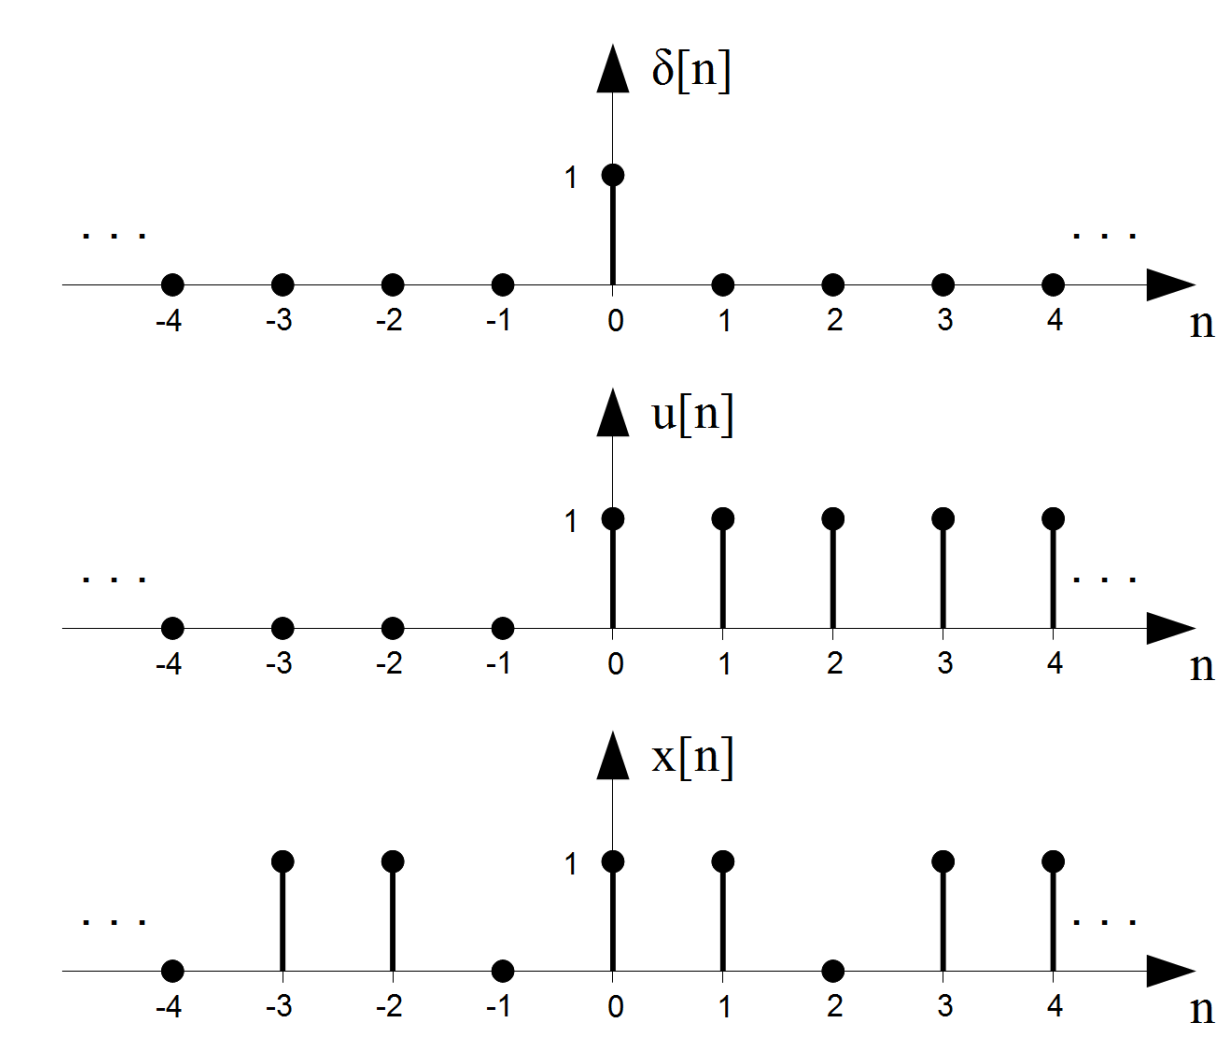
\includegraphics[scale=.7]{./images/basic_signals}
\end{center}

Komplexe harmonische Sequenz:
\[ x[n] = \hat{X} \cdot \e^{\im 2 \pi f_0 n T_S} \]
Real- und Imaginäranteil der komplexen Harmonischen:
\[ Re\{\} = \hat{X} \cdot \cos 2 \pi f_0 n T_S \]
\[ Im\{\} = \hat{X} \cdot \sin 2 \pi f_0 n T_S \]

%===============================================================================
\subsection{Statistische Signalparameter}
Observations Intervall $T$:
\[ T = N \cdot T_S \]
Der Mittelwert (\textbf{mean value}) $\mu_x$ repräsentiert
den DC-Anteil des Signals x[n]:
\[ \mu_x = \frac{1}{N} \sum_{i=0}^{N-1}x[i] \]
Der quadratische Mittelwert (\textbf{quadratic mean value}) ${\rho_x}^2$
korrespondiert zur durchschnittlichen Leistung des Signal $x[n]$
mit DC-Anteil:
\[ {\rho_x}^2 = \frac{1}{N} \sum_{i=0}^{N-1} x[i]^2 \]
Die \textbf{Varianz} ${\sigma_x}^2$ repräsentiert die durchschnittliche
AC-Leistung des Signals $x[n]$:
\[ {\sigma_x}^2 = \frac{1}{N} \sum_{i=0}^{N-1}(x[i] - \mu_x)^2 \]

%===============================================================================
\subsection{Messverhältnisse und dB}
Leistungsverhältnis (\textbf{power ratio}):
\[ A_{dB} = 10 \cdot \log_{10} \left( \frac{P_1}{P_2} \right) \]
Signal-to-noise ratio (\textbf{SNR}):
\[ SNR_{dB} = 10 \cdot \log_{10} \left( \frac{P_{signal}}{P_{noise}} \right) \]

\begin{table}[ht]
  \centering
  \begin{tabular}{ccc} \toprule
  Linear	& \multicolumn{2}{c}{Power ratio [dB]} \\ 
  $a/b$		& Power		& Voltage	\\ \midrule
  $1/1000$	& -30		& -60		\\
  $1/100$	& -20		& -40		\\
  $1/10$	& -10		& -20		\\
  $1/2$		& $\approx -3$& $\approx -6$\\
  $1$		& 0			& 0			\\
  $2/1$		& $\approx -3$& $\approx 6$\\
  $10/1$	& 10		& 20		\\
  $100/1$	& 20		& 40		\\  \bottomrule
  \end{tabular}
\end{table}

%===============================================================================
\section{Signal Operationen}
\subsection{Korrelation}
Die statische Korrelation (\textbf{static correlation}) drückt die Ähnlichkeit
zweier Signale x[n] und y[n] der selben Länge $N$ aus:
\[ R = \frac{1}{N} \sum_{i=0}^{N-1} x[i]y[i] \]
Je ähnlicher sich die Signale sind, desto grösser der Wert $R$.\\\\
Die lineare Korrelationsfunktion (\textbf{linear correlation fucntion}):
\[ r_{xy}[n] = \sum_{i=-\infty}^{\infty} x[i]y[i+n] \]
Die Korrelation ist nicht kommutativ, $r_{xy}[n] \neq r_{yx}[n]$.\\\\
Resultierende Länge von $r_{xy}$:
\[ N_{xy} = N_x + N_y - 1 \]
~\\
Mathlabbefehl für Kreuz- und Autokorrelation: \verb|xcorr|

\subsection{Faltung}
Die Faltung (\textbf{convolution}) ist definiert als:
\[ z[n] = \sum_{i=-\infty}^{\infty} x[i]y[-i+n] \]
Die Faltung ist kommutativ:
\[ z[n] = x[n] * y[n] = y[n] * x[n] \]
Resultierende Länge für $z[n]$:
\[ N_z = N_x + N_y -1 \]
Bei der zyklischen Faltung (\textbf{circular convolution}) müssen die beiden
Signale die selbe Länge $N$ haben, oder mit Zero-Padding auf die selbe Länge
gebracht werden:
\[ z[n] = x[n] \circledast_N y[n] = y[n] \circledast_N x[n] \]
Lösung durch Matrix:
\[
	\begin{bmatrix}
		y[N]	& y[N-1]	& \ldots & y[0] \\
		y[0]	& y[N]		& \ddots & y[1] \\
		\ddots	& \ddots	& \ddots & \ddots \\
		y[N-1]	& y[N-2]	& \ldots & y[N]
	\end{bmatrix} \cdot \begin{bmatrix}
		x[0] \\ x[1] \\ \vdots \\ x[N]
	\end{bmatrix} = \begin{bmatrix}
		z[0] \\ z[1] \\ \vdots \\ z[N]
	\end{bmatrix}
\]
~\\\\
Mathlabbefehl für Faltung: \verb|conv|\\
Mathalbbefehl für zyklische Faltung: \verb|convmtx|
% coding:utf-8

%----------------------------------------
%FOSADSVB, a LaTeX-Code for a summary of digital signal processing
%Copyright (C) 2015, Mario Felder & Michi Fallegger

%This program is free software; you can redistribute it and/or
%modify it under the terms of the GNU General Public License
%as published by the Free Software Foundation; either version 2
%of the License, or (at your option) any later version.

%This program is distributed in the hope that it will be useful,
%but WITHOUT ANY WARRANTY; without even the implied warranty of
%MERCHANTABILITY or FITNESS FOR A PARTICULAR PURPOSE.  See the
%GNU General Public License for more details.
%----------------------------------------

\chapter{Analog-Digital \& Digital-Analog Wandlung}
\section{Schritte der A/D- und D/A-Wandlung}
\paragraph{Sample:} Kontinuierliche Signalwerte werden mit der Samplefrequenz
$f_S$ aufgezeichnet. Dies erzeugt eine Sequenz von diskreten Signalwerten.

\paragraph{Quantize:} Die diskreten Signalwerte werden einer bestimmten
Anzahl Quantisierungsleveln zugeordnet.

\paragraph{Code:} Die quantisierten Abtastwerte können verwendet werden,
um die erhaltene Pulsfolge zu modulieren (Pulse Code Modulation PCM). Meistens
wird die Signalverarbeitung direkt mit den quantisierten Abtastwerten vorgenommen,
so dass diese ohne Modulation gespeichert werden. Dazu wird die Repräsentierung
der Quantisierungsleveln benötigt.\\
\\
Die Digital-Analog Wandlung enthält folgende Schritte:\\
\paragraph{Decode:} Die digitalen Werte werden in einer für die Digital-Analog
Wandlung repräsentativer Form benötigt.

\paragraph{Hold:} Das diskrete Signal muss über die Sampleperiode $T_S$ konstant
gehalten werden, ein Treppen ähnlicher Output entsteht.

\paragraph{Interpolate:} Das kontinuierliche Treppensignal wird durch Mittelwerte
von Tiefpass-Filtern geglättet.

\begin{center}
	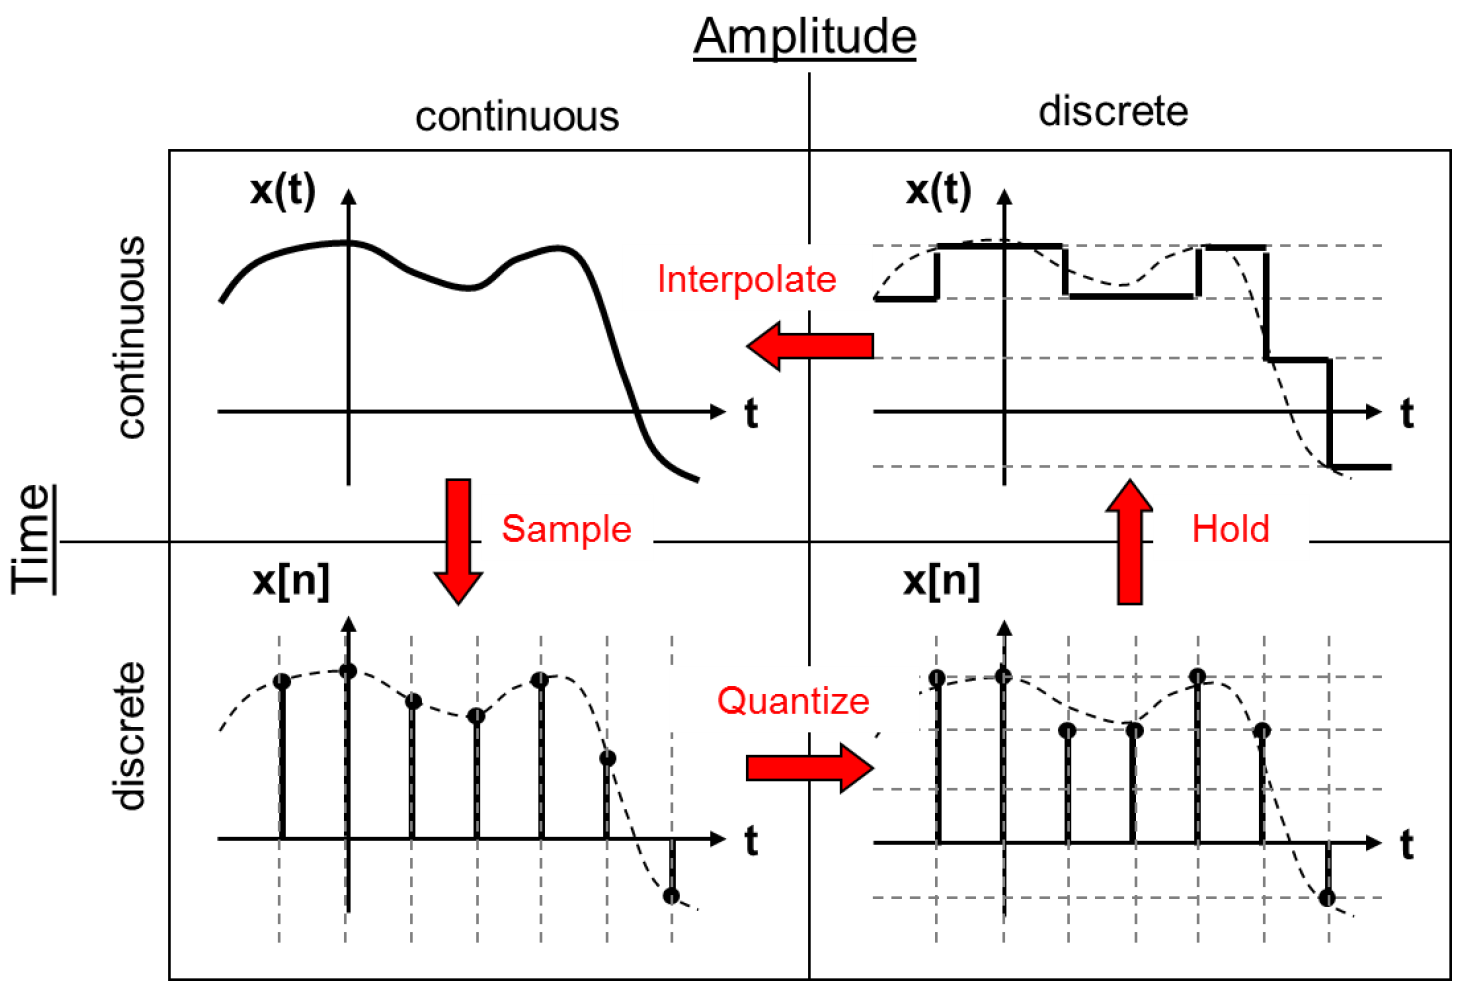
\includegraphics[scale=.7]{./images/ad_da}
\end{center}

%===============================================================================
\section{Abtasten und Aliasing}
\subsection{Abtasten von Tiefpass Signalen}
Mathematisch wird die Abtastung des Signals $x(t)$ durch eine Multiplikation
mit Dirac-Impulsen der Periode $T_S$ dargestellt:
\[ x_s(t) = \sum_{n=-\infty}^{\infty} x(t) \cdot \delta(t-nT_S) \]
Das Frequenzspektrum des abgetasteten Singals ist:
\[ X_S(f) = \frac{1}{T_S} \sum_{k-\infty}^{\infty} X(f-kf_S) \]

\begin{center}
	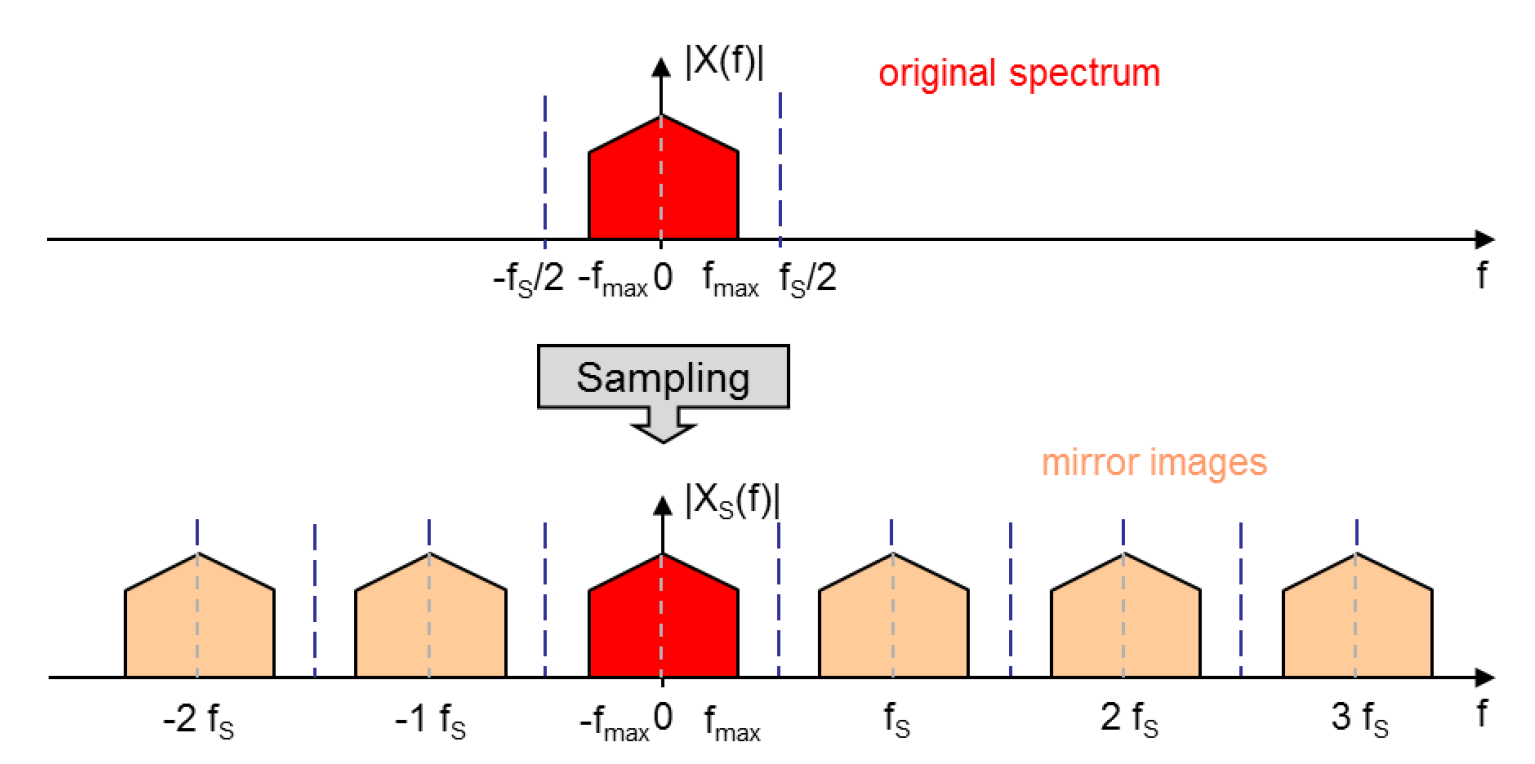
\includegraphics[scale=.7]{./images/frequenz_spectrum}
\end{center}
Um das Signal rekonstruieren zu können, müssen die Spiegelfrequenzen von $X(f)$
mit einem Tiefpassfilter unterdrückt werden. Das geht nur, wenn die grösste
Frequenz $f_{max}$ des Signals kleiner als die halbe Abtastfrequenz $f_S/2$ ist.
\[ f_S > 2 \cdot f_{max} \]

%===============================================================================
\subsection{Aliasing}
Aliasing entsteht, wenn das Abtasttheorem verletzt wird. Die Frequenzanteile
über $f_S/2$ werden in das Basisband gespiegelt und überlagern mit den 
gewünschten Frequenzen. Das analoge Signal kann nicht rekonstruiert werden.\\
\\
Dem kann mit einer Tiefpassfilterung entgegengewirkt werden. Der Filter hat
folgende Spezifikationen:
\[ f_{pass} \geq f_{desired} \]
\[ f_{stop} \leq f_S - f_{desire} \]

\begin{center}
	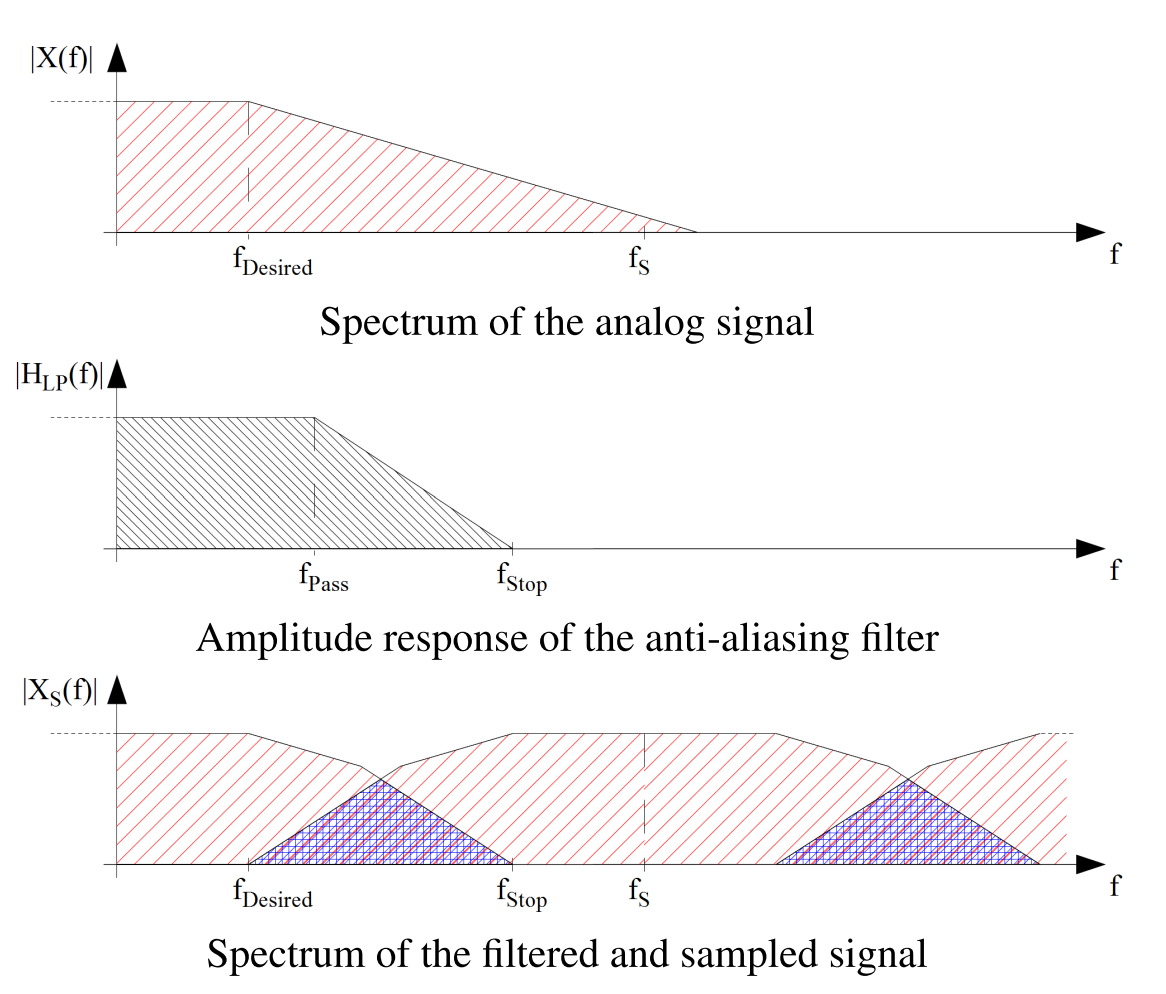
\includegraphics[scale=.7]{./images/aliasing}
\end{center}

%===============================================================================
\subsection{Abtasten von Bandpass Signalen}
Das Abtasttheorem wird folgendermassen angepasst (für $N\geq 1$):
\[ \frac{2\cdot f_{min}}{N} \geq f_S \geq \frac{2\cdot f_{max}}{N+1} \]
Für ungerade $N$ erscheint das originale Spektrum invertiert im Basisband.
Die originale Struktur des Spektrum wird zurückgewonnen durch invertierung
jedes zweiten Samples im Zeitbereich:
\[ \tilde{x}[n] = (-1)^n \cdot x[n] \]

\begin{minipage}{.5\textwidth}
	\begin{center}
		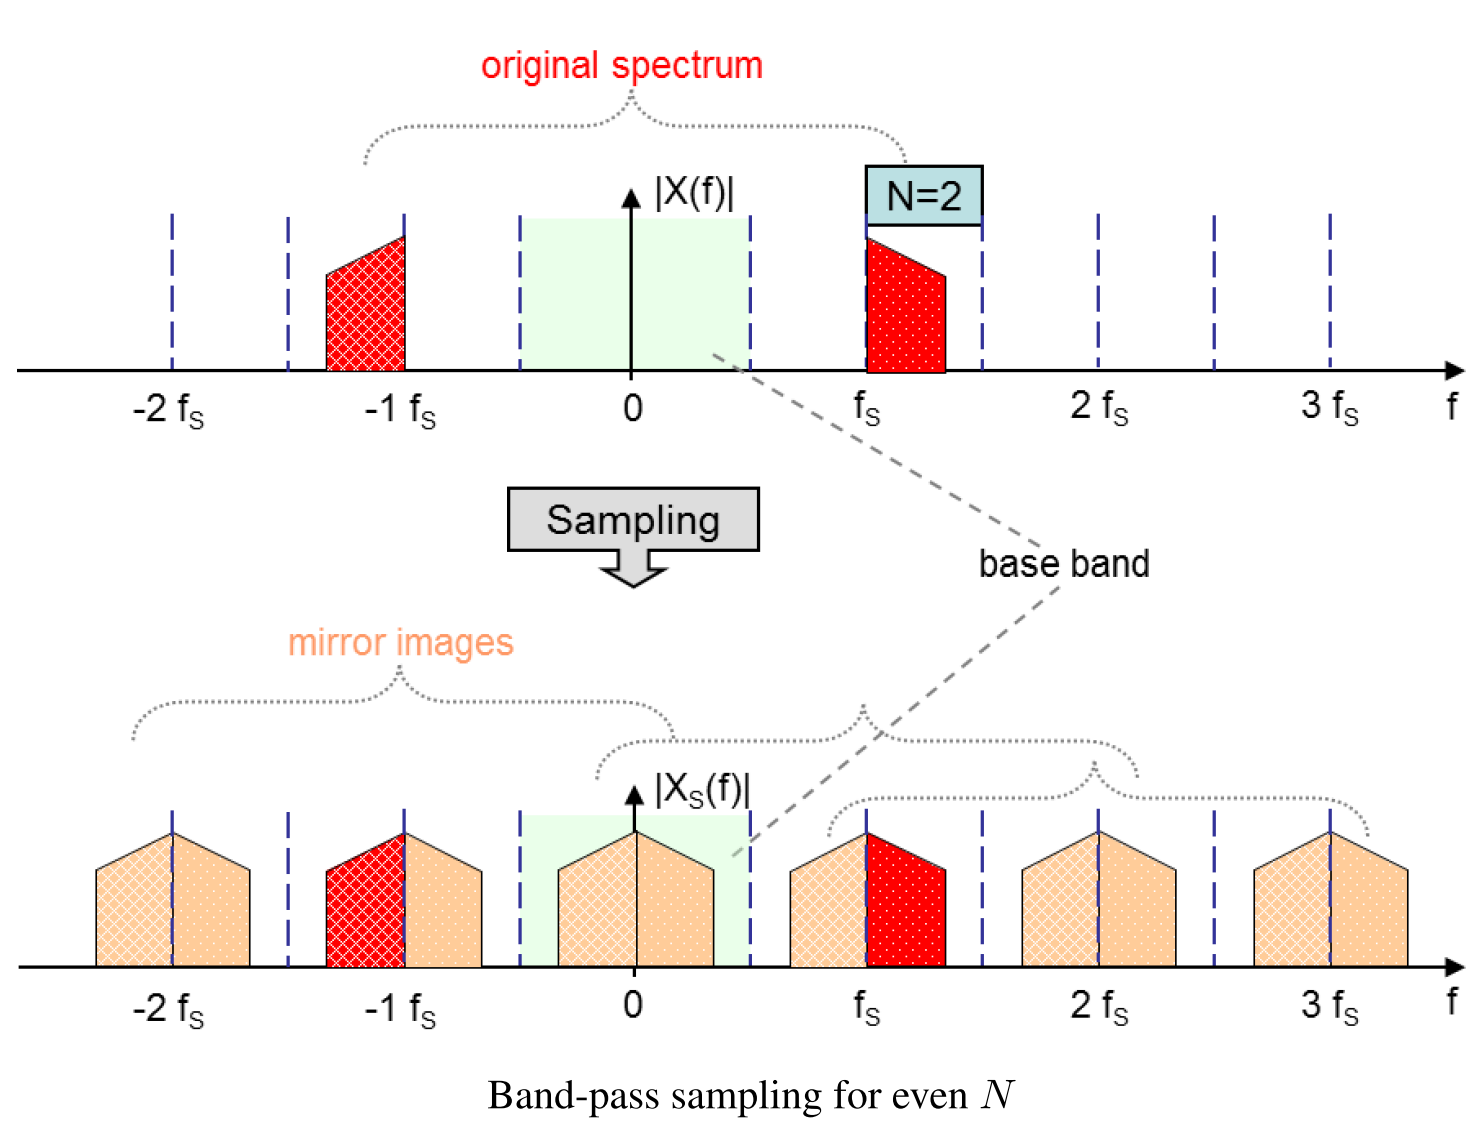
\includegraphics[width=\textwidth]{./images/bandpass_even}
	\end{center}
\end{minipage}
\begin{minipage}{.5\textwidth}
	\begin{center}
		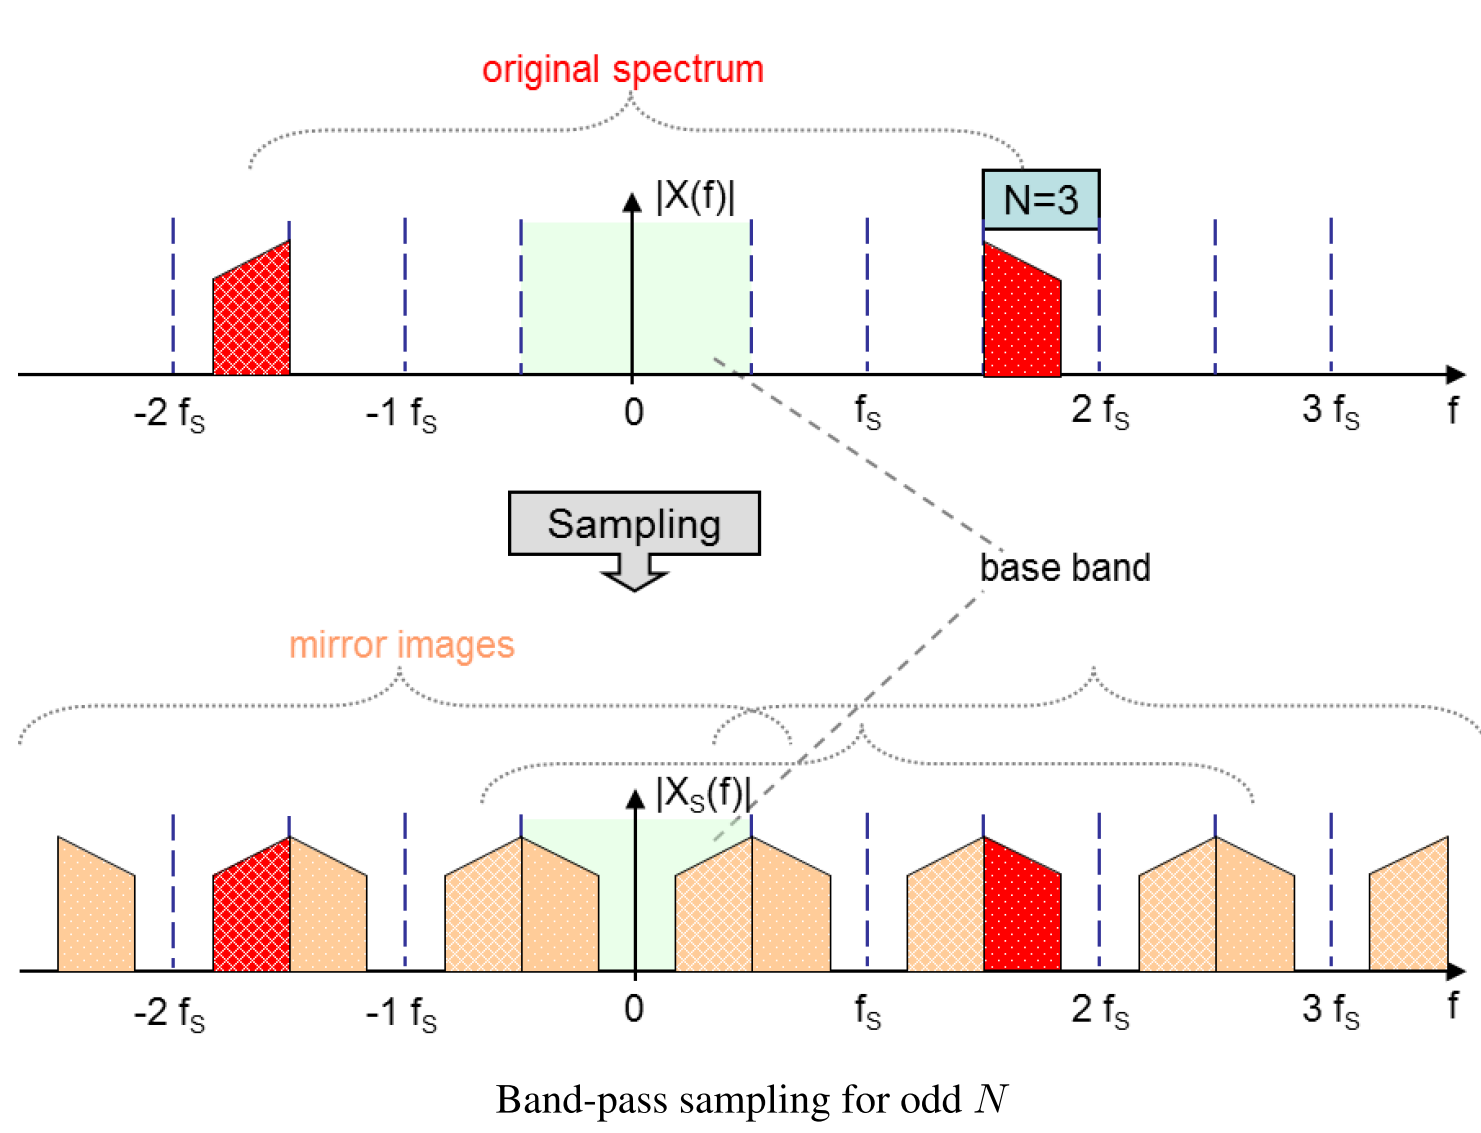
\includegraphics[width=\textwidth]{./images/bandpass_odd}
	\end{center}
\end{minipage}

%===============================================================================
\section{Quantisierung von Signalen}
\subsection{Uniforme Quantisierung}
Der Quantisierungsschritt (\textbf{quantization step}) $\Delta$ ist gegeben
durch die Auflösung mit $W$ bits und der dynamischen Reichweite $R$ des
abgetasteten Signals $x[n]$:
\[ \Delta = \frac{R}{2^W} \]
Durch das Abbilden eines amplitudenkontinuierlichen Signals auf eine endliche
Anzahl von Rekonstruktionsleveln können zweier Fehler entstehen:\\
\paragraph{Clipping:} Werte von $x[n]$ ausserhalb des Bereichs $R$ werden mit
dem maximum bzw. minimum Rekonstruktionslevel dargestellt.

\paragraph{Quantization error $\epsilon$:} Dieser Fehler tritt immer auf und
kann nicht verhindert werden. Die Grösse des Fehlers ist gegeben durch die
Qunatisierungsgrösse $\Delta$.\\

Für den mid-tread quantizer (runden zum nächsten Wert):
\[ -\Delta/2 < \epsilon \leq \Delta / 2 \]

Für den mid-rise quntizer:
\[ -\Delta < \epsilon \leq 0 \]

%===============================================================================
\subsection{Quantisierungsrauschen}
Der Quantisierungsfehler zeigt sich als Rauschen überlagert zum quantisierten
Signal:
\[ \epsilon[n] = x_q[n] - x[n] \]
Die Leistung $P_\epsilon$ des Quantisierungsrauschens
(\textbf{quantization noise}) ist:
\[ P_\epsilon = {\sigma_\epsilon}^2 = \int_{-\infty}^{\infty} (\epsilon - 
	{\sigma_\epsilon})^2 \cdot p(\epsilon) \di\epsilon = 
	\frac{\Delta^2}{12}\]
wobei $p(\epsilon)$ die Wahrscheinlichkeitsdichte ist. Angenommen die Werte
von $\epsilon[n]$ sind statistisch unkorreliert und uniform verteilt über den
Intervall $(-\Delta/2, \Delta/2]$ ist die Wahrscheinlichkeitsdichte für einen
mid-tread quantizer:
\[ p(\epsilon) = 1/\Delta \] 
Der Erwartungswert des Quantisierungsfehlers ist somit:
\[ \mu(\epsilon) = \int_{-\infty}^{\infty} \epsilon \cdot p(\epsilon) 
	\di\epsilon = \left. \frac{1}{2\Delta}\epsilon^2
	\right|_{-\Delta/2}^{\Delta/2} = 0 \]

\begin{center}
	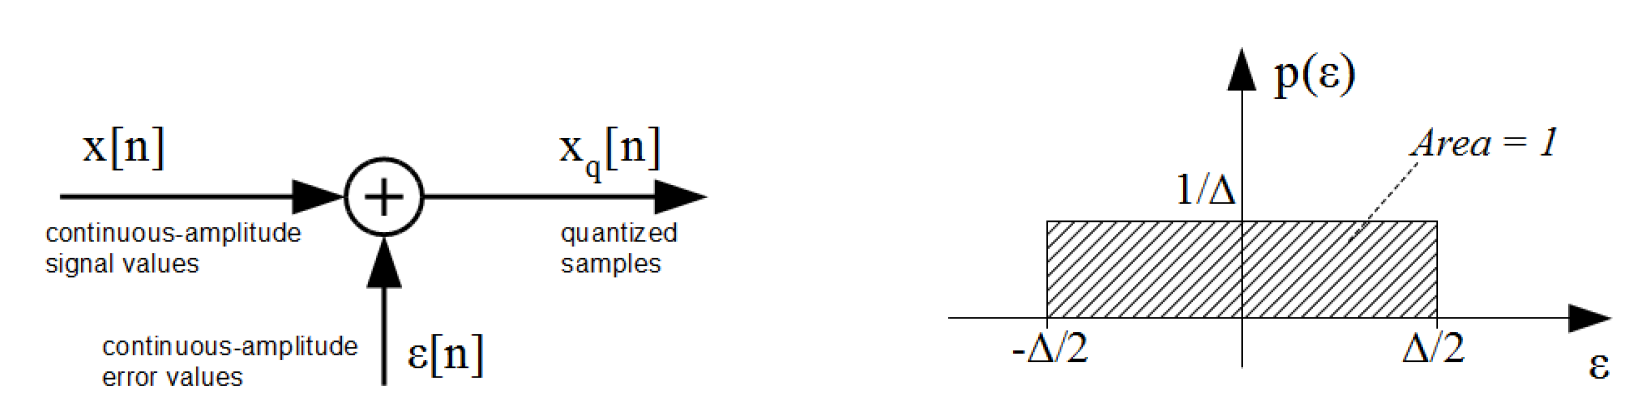
\includegraphics[width=.9\textwidth]{./images/quantization_noise}
\end{center}
Das SNR ist:
\[ SNR = \frac{P_x}{P_\epsilon} = 2^{2W} \cdot \frac{12P_x}{R^2} \]
\[\begin{aligned} SNR_{dB} &= 10 \cdot \left( \log_{10}2^{2W} +
	 \log_{10}\frac{12P_x}{R^2} \right)\\
	 &\approx 6W + 10 \cdot \log_{10}\frac{12P_x}{R^2} 
\end{aligned}\]
Bei einem harmonischen Inputsignal $x[n]$ ergibt sich folgendes SNR für
eine uniforme Quantisierung:
\[ SNR_{db} = 6W +1.76 \approx 6W \]
% coding:utf-8

%----------------------------------------
%FOSADSVB, a LaTeX-Code for a summary of digital signal processing
%Copyright (C) 2015, Mario Felder & Michi Fallegger

%This program is free software; you can redistribute it and/or
%modify it under the terms of the GNU General Public License
%as published by the Free Software Foundation; either version 2
%of the License, or (at your option) any later version.

%This program is distributed in the hope that it will be useful,
%but WITHOUT ANY WARRANTY; without even the implied warranty of
%MERCHANTABILITY or FITNESS FOR A PARTICULAR PURPOSE.  See the
%GNU General Public License for more details.
%----------------------------------------

\chapter{Digitale Signale im Frequenzbereich}
\section{Von Fourier Tranformation zur DFT}
\subsection{Übergang zu diskreter Zeit}
Die zeitdiskrete Fourier Transformation (DTFT) kann berechnet werden mit:
\[ X(\Omega) = \sum_{n=-\infty}^{\infty} x[n]\e^{-\im\Omega n} \]
mit der normalisierten Winkelfrequenz:
\[ \Omega = 2\pi f T_S = 2\pi\frac{f}{f_S} \]
Die DTFT produziert ein $2\pi$-periodisches, kontinuierliches Spektrum.

%===============================================================================
\subsection{Übergang zu endlichem Messintervall}
Wenn nur über $N$ Abtastpunkte eine Fourier Analyse gemacht werden soll,
ist die kleinste Frequenz, welche aufgenommen werden kann:
\[ f_1 = \frac{1}{T} = \frac{1}{N \cdot T_S} = \frac{f_S}{N} \]
Die Diskrete Fourier Transformation (DFT) kann geschrieben werden als:
\[ X[k] = \sum_{n=0}^{N-1}x[n] \e^{-\im 2 \pi n \frac{k}{N}} \qquad 
	k = 0,1, 2, \ldots , N-1 \]
Die DFT ist beschränkt zu einer maximalen Frequenz von:
\[ (N-1)\frac{f_S}{N} \]
Die inverse diskrete Fourier Transformation (IDFT) ist gegeben durch:
\[ x[n] = \frac{1}{N} \sum_{k=0}^{N-1} X[k]\e^{\im 2\pi n \frac{k}{N}} 
	\qquad n = 0,1, 2, \ldots , N-1 \]
	
\begin{center}
	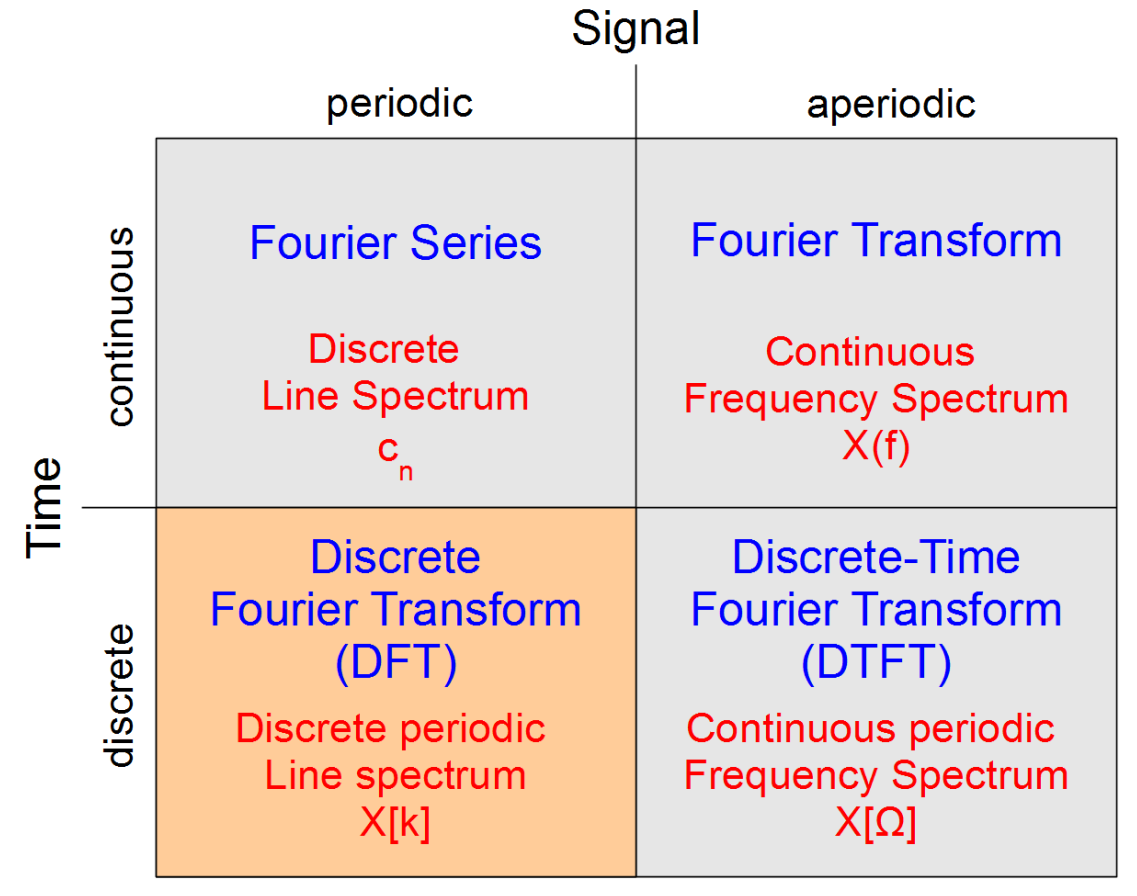
\includegraphics[scale=.7]{./images/fft_methods}
\end{center}

%===============================================================================
\section{Eingenschaften der DFT}
\textbf{Periodizität}\\
Das Spektrum der DFT ist $f_S$-periodisch
\[ X[k] = X[k+N] \]
Dementsprechend ist IDFT periodisch mit $T=NT_S$
\[ x[n] = x[n+N] \]\\
\\
\textbf{Symmetrie}\\
Die DFT eines realwertigen Signals ist symmetrisch um den Punkt $k=N/2$
\[ X[N/2+m] = X^*[N/2-m] \]\\
\\
\textbf{Zeit/Frequenz Verschiebung}\\
Verschiebung einer periodischen Zeitsequenz um $n_0$ hat einen linearen Phasen
Offset bei allen Spektralwerten zur Folge
\[ x[n+n_0] \qquad \laplace \qquad \e^{\im 2\pi n_0 \frac{k}{N}} \cdot X[k] \]
Die Multiplikation mit einem komplexen Exponent hat eine konstante
Frequenzverschiebung zur Folge
\[ \e^{\im 2\pi k_0 \frac{n}{N}} \cdot x[n] \qquad \laplace \qquad X[k-k_0] \]\\
\\
\textbf{Modulation}\\
Konsequenz der Frequenzverschiebung ist die Modulation
\[ \cos\left(2\pi k_0\frac{n}{N}\right) \cdot x[n] \qquad\laplace\qquad
	\frac{1}{2}\left( X[k+k_0] + X[k-k_0] \right) \]\\
\\
\textbf{Parseval Theorem}\\
Zwischen Signalwerten $x[k]$ und Fourier Koeffizienten $X[k]$ besteht folgende
Beziehung:
\[ \frac{1}{N} \sum_{n=0}^{N-1}x[n]^2 = \sum_{k=0}^{N-1}\left| 
	\frac{X[k]}{N} \right|^2  \]\\
\\
\textbf{Zusammenhang von Faltung und Multiplikation}\\
Punktweise Multiplikation zweier DFT Spektren $X[k]$ und $Y[k]$ im 
Frequenzbereich entspricht der zyklischen Faltung von $x[n]$ und $y[n]$ im 
Zeitbereich
\[ x[n] \circledast_N y[n] \qquad\laplace\qquad X[k]\cdot Y[k] \]

%===============================================================================
\subsection{Gültigkeitsbereich der DFT}
\[ X[k] = X[\Omega]|_{\Omega=2\pi\frac{k}{N}} \]
\textbf{$x[n]$ periodisch:}\\
Der Messintervall $NT_S$ ist ein ganzzahliger Vielfache der Periodendauer
von $x[n] $.\\
\\
\textbf{$x[n]$ aperiodisch:}\\
Alle Werte von $x[n]$ ausserhalb dem Bereich $0\geq n<N$ sind Null.

%===============================================================================
\section{Anwendungs Aspekte}
\subsection{Zero-Padding}
Um eine bessere Interpolation zwischen den $N$ Frequenzpunkten in der DFT zu
bekommen, kann das Signal im Zeitbereich mit Nullen aufgefüllt werden.
Das Spektrum $X(\Omega)$ wird nicht verändert, allerdings stehen zusätzliche
Abtastpunkte auf der Achse der normalisierten Winkelfrequenz zu Verfügung.

%===============================================================================
\subsection{Fensterfunktion}
Die DFT wendet per Definition ein Rechteckfenster an, um die $N$ Samples
auszuschneiden. Es können andere Fensterfunktionen auf das Signal $x[n]$
angewendet werden, allerdings gelten folgende Punkte:
\begin{itemize}
	\item Je schmaler die Hauptkeule im Spektrum des Fensters, desto höher ist
	die spektrale Auflösung für $X[k]$
	\item Je stärker die Dämpfung der Nebenkeulen im Spektrum des Fenster, desto
	besser die Unterdrückung der Leackage in $X[k]$
\end{itemize}

\begin{center}
	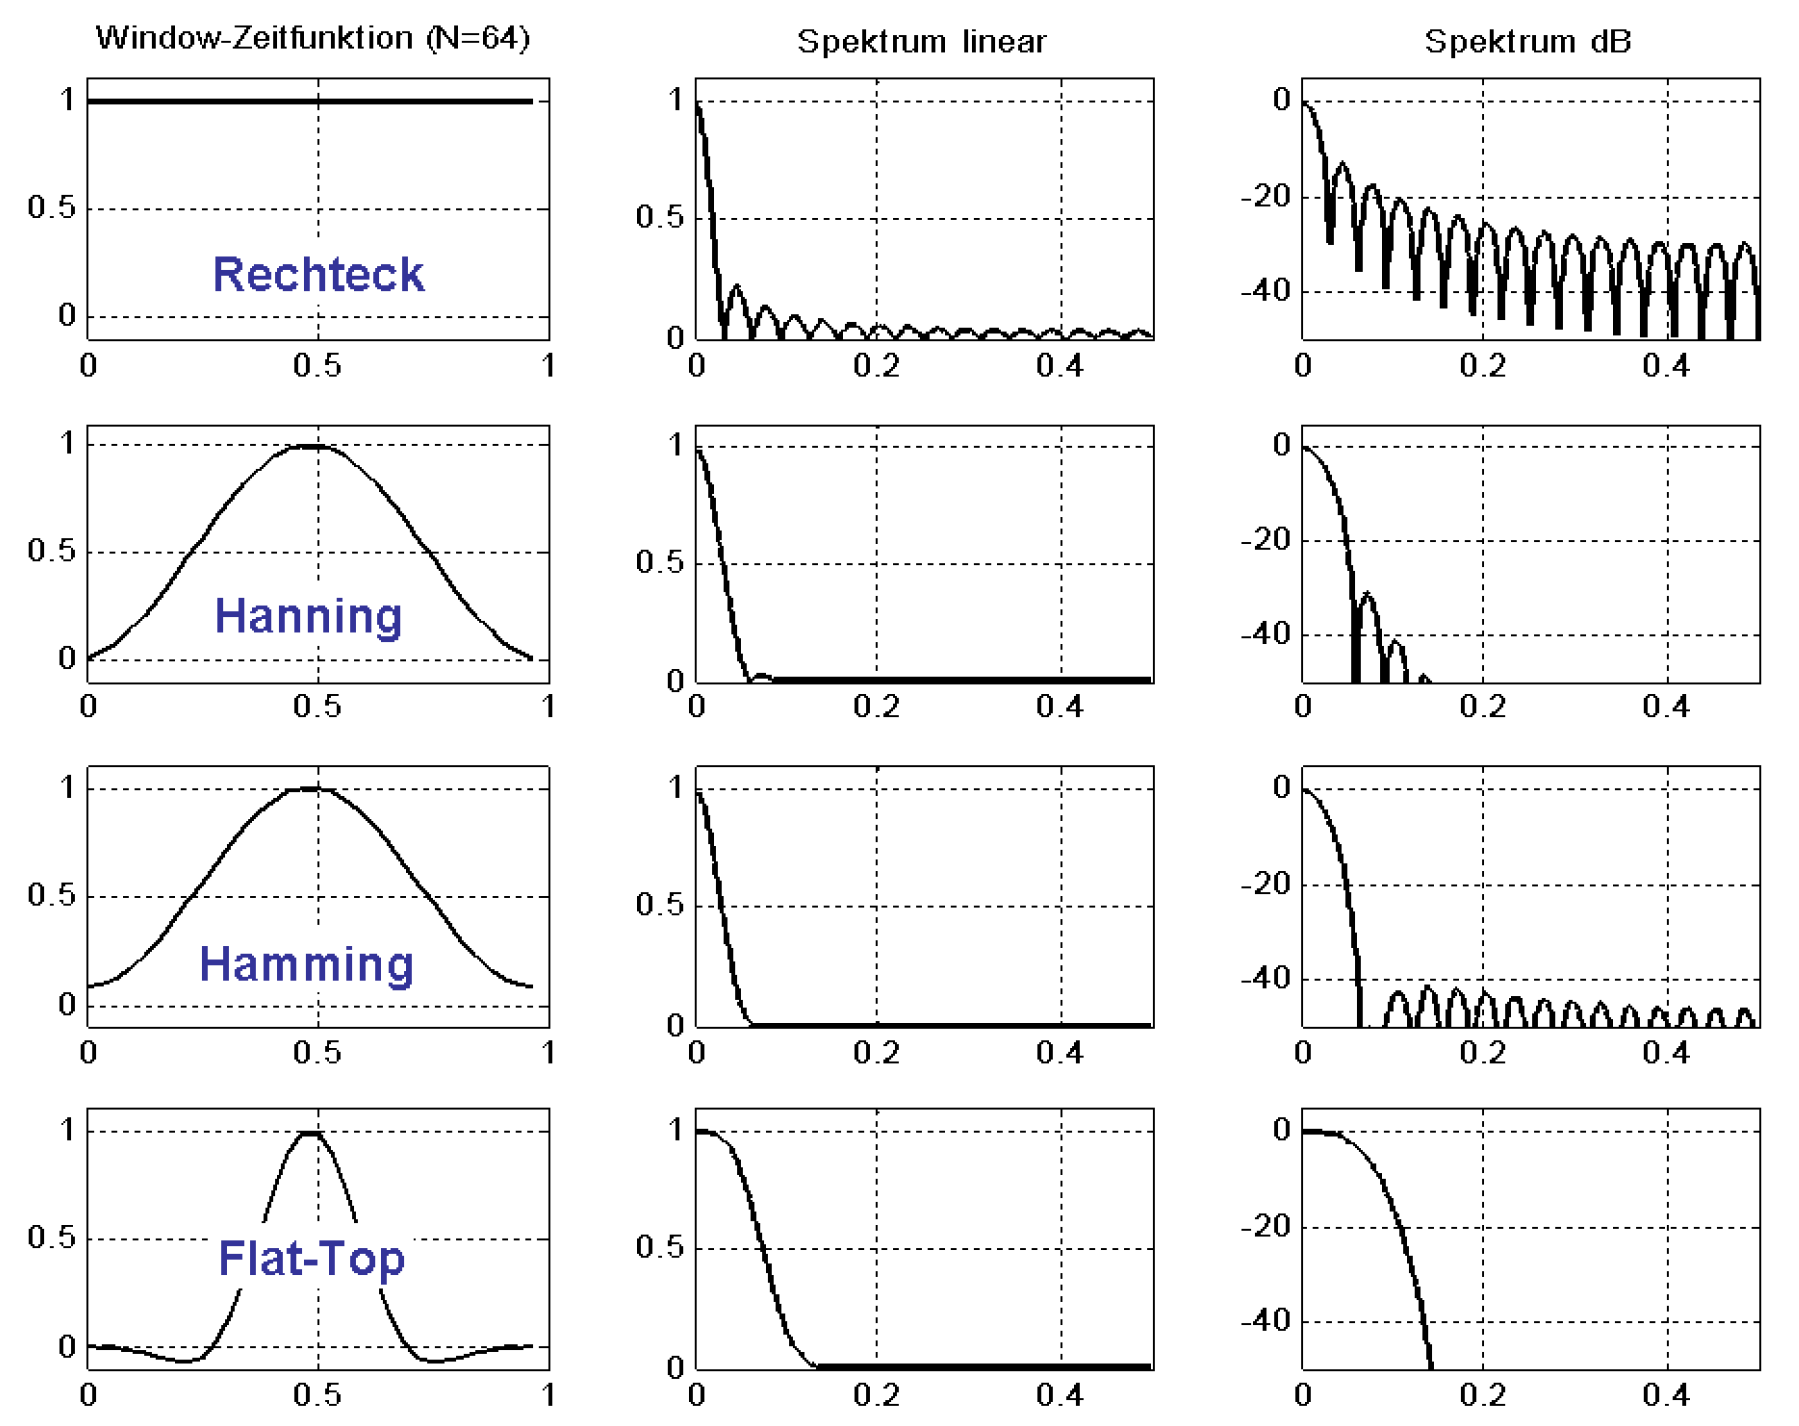
\includegraphics[scale=.7]{./images/windows}
\end{center}

%===============================================================================
\section{Short-Time DFT}
Wenn die Entwicklung des Frequenzspektrums über die Zeit interessiert, werden
kontinuierliche Berechnungen des Spektrums von kurzen Signalsektoren 
durchgeführt. Da diese kurzen Sektoren meistens nicht ein ganzzahliges
vielfache Vielfache der Periode ist, werden Fensterfunktionen angewendet.\\
\\
Bei der Länge $N$ des Fensters ergibt sich der Kompromiss von:
\begin{itemize}
	\item grosse spektrale Auflösung ($N$ gross)
	\item grosse zeitliche Auflösung ($N$ klein)
\end{itemize}

Um beides zu erreichen, können die DFT-Fenster überlappt werden um maximal
$N-1$.

%===============================================================================
\section{Fast Fourier Transformation (FFT)}
Geschwindigkeitsvergleich FFT-DFT:
\[ speedup\_factor_{FFT} = \frac{8N-2}{5\cdot \log_2N} \approx 1.5 	
	\frac{N}{\log_2N} \]
Dabei ist $N = 2^L$ mit einem ganzzahligen Wert für $L$.

%===============================================================================
\subsection{Twiddle Faktoren}
Definition:
\[ W_N = \e^{-\im\frac{2\pi}{N}} \]\\
\\
\textbf{Periodizität}\\
$W_N$ kann nur für $N$ verschiedene Zahlen ausgewertet werden. Der Twiddle
Faktor ist somit $N$-periodisch
\[ W_N^{k+N} = W_N^k \]\\
\\
\textbf{Symmetrie}\\
Abgesehen vom Vorzeichen nimmt $W_N$ nur $N/2$ verschiedene Werte an.
\[ W_N^{k+N/2} = -W_N^k \]

%===============================================================================
\subsection{Radix-2 FFT}
Die DFT wird mit dem Twiddle Faktor umgeschrieben:
\[\begin{aligned} X[k] &= \sum_{n=0}^{N-1} x[nW_N^{nk}]\\
	&= \sum_{n \textrm{ even}} x[n]W_N^{nk} + \sum_{n\textrm{ odd}}x[n]W_N^{nk}
\end{aligned}\]
Es können zwei neue Sequenzen $x_1[n]$ und $x_2[n]$ mit geraden und ungeraden
$n$ von der Länge $N/2$ erzeugt werden.
\[ X[k] = \underbrace{\sum_{n=0}^{N/2-1}x_1[n]W_{N/2}^{nk}}_{x_1[\tilde{k}]} +
	W_N^k\cdot \underbrace{\sum_{n=0}^{N/2-1} x_2[n]W_{N/2}^{nk}}_
	{{x_2[\tilde{k}]}} \]
wobei
\[ \tilde{k} = k\mod N/2 \]

\begin{center}
	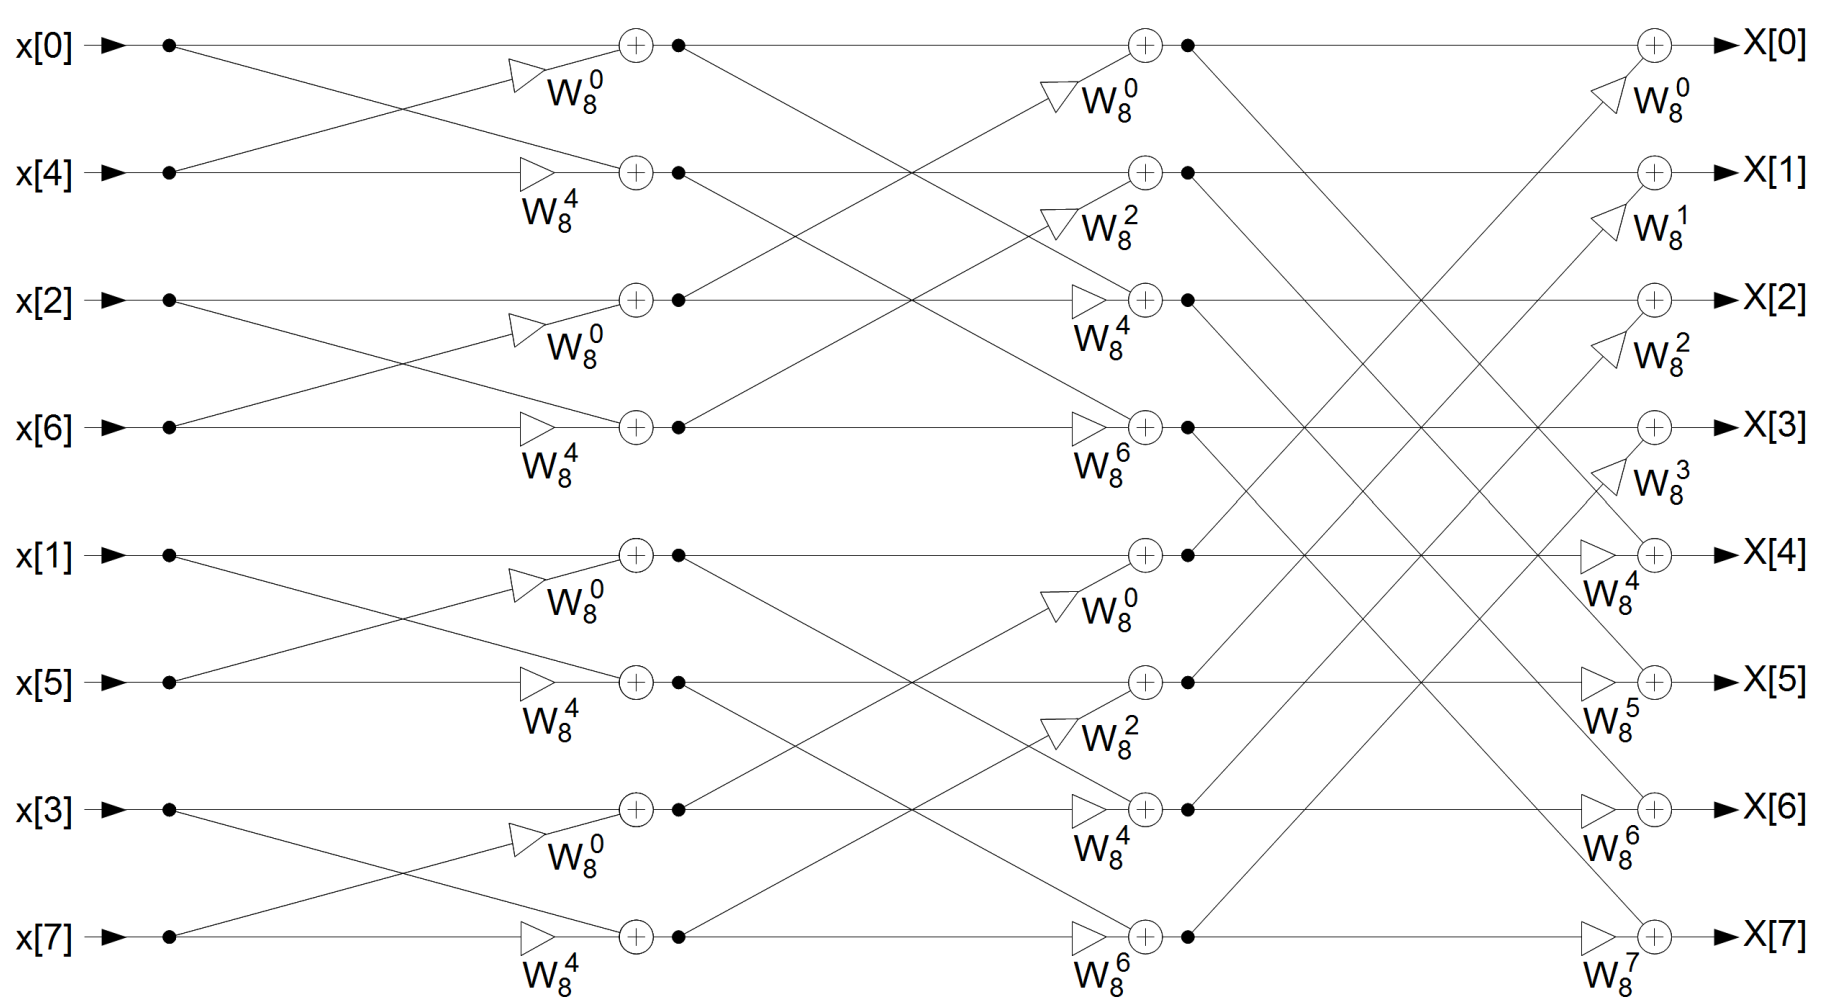
\includegraphics[scale=.7]{./images/fft}
\end{center}

Index bit-reversed in Matlab: \verb|bitrevorder|

%===============================================================================
\section{Goertzel-Algorithmus}
Definition:
\[ X[k] = y_k[n]|_{n=N} = \sum_{i=0}^{N-1}x[i]W_N^{-k(N-i)} \]
Differenzengleichung:
\[ s[n] = x[n] + a \cdot s[n-1] - s[n-2] \]
\[ y_k[n] = s[n] - W_N^k \cdot s[n-1] \]
mit 
\[ a= 2\cos 2\pi\frac{k}{N} \]
$s[n]$ muss für alle Zeitpunkte $n=0,1,\ldots,N$ berechnet werden, $y_k[n]$
nur für $n=N$.

\begin{center}
	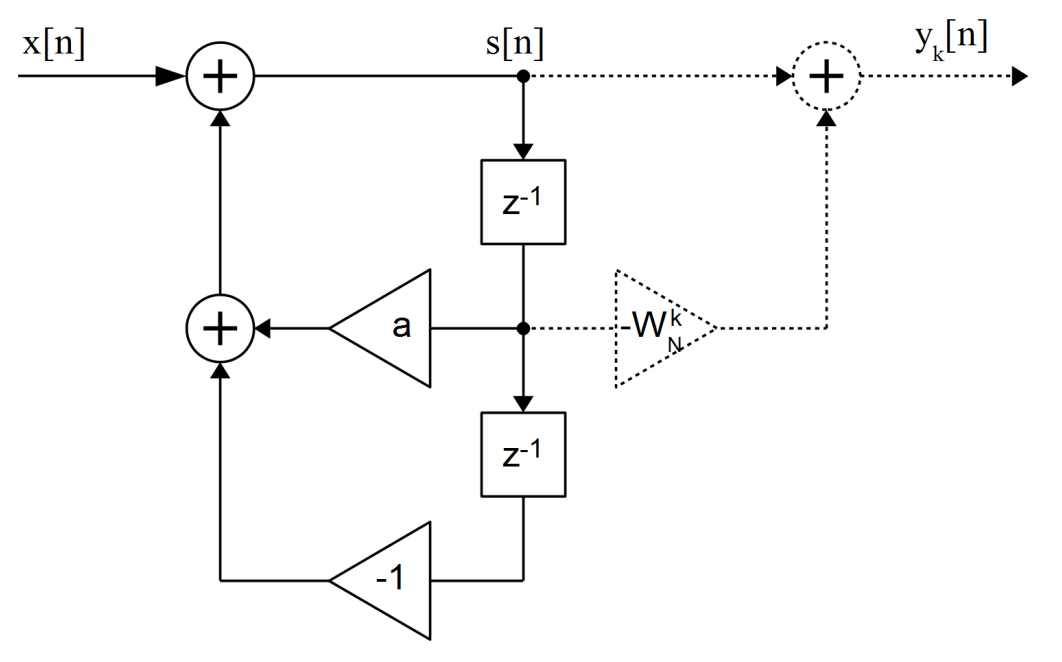
\includegraphics[scale=.7]{./images/goertzel}
\end{center}
Der Goertzel-Algorithmus gibt die DFT spectral componente bei der Frequenz
\[ f_k = k\frac{f_S}{N} \]
Mit dem PArseval Theorem kann der Leistungsgehalt $P_k$ eines realwertigen
Signals $x[n]$ bei einer Frequenz von $f_k$ ermittelt werden:
\[
	P_k = 2\left| \frac{X[k]}{N} \right|^2
		= \frac{2}{N^2}(\Re\{X[k]\}^2+\Im\{X[k]\}^2)
\]
% coding:utf-8

%----------------------------------------
%FOSADSVB, a LaTeX-Code for a summary of digital signal processing
%Copyright (C) 2015, Mario Felder & Michi Fallegger

%This program is free software; you can redistribute it and/or
%modify it under the terms of the GNU General Public License
%as published by the Free Software Foundation; either version 2
%of the License, or (at your option) any later version.

%This program is distributed in the hope that it will be useful,
%but WITHOUT ANY WARRANTY; without even the implied warranty of
%MERCHANTABILITY or FITNESS FOR A PARTICULAR PURPOSE.  See the
%GNU General Public License for more details.
%----------------------------------------
\chapter{Digitales Filterdesign}
Ziel: Bestimmen der Parameter $b_k$ \& $a_k$, sowie der Ordnung $N$ \& $M$ für gegebene Filterspezifikationen.
\begin{center}
	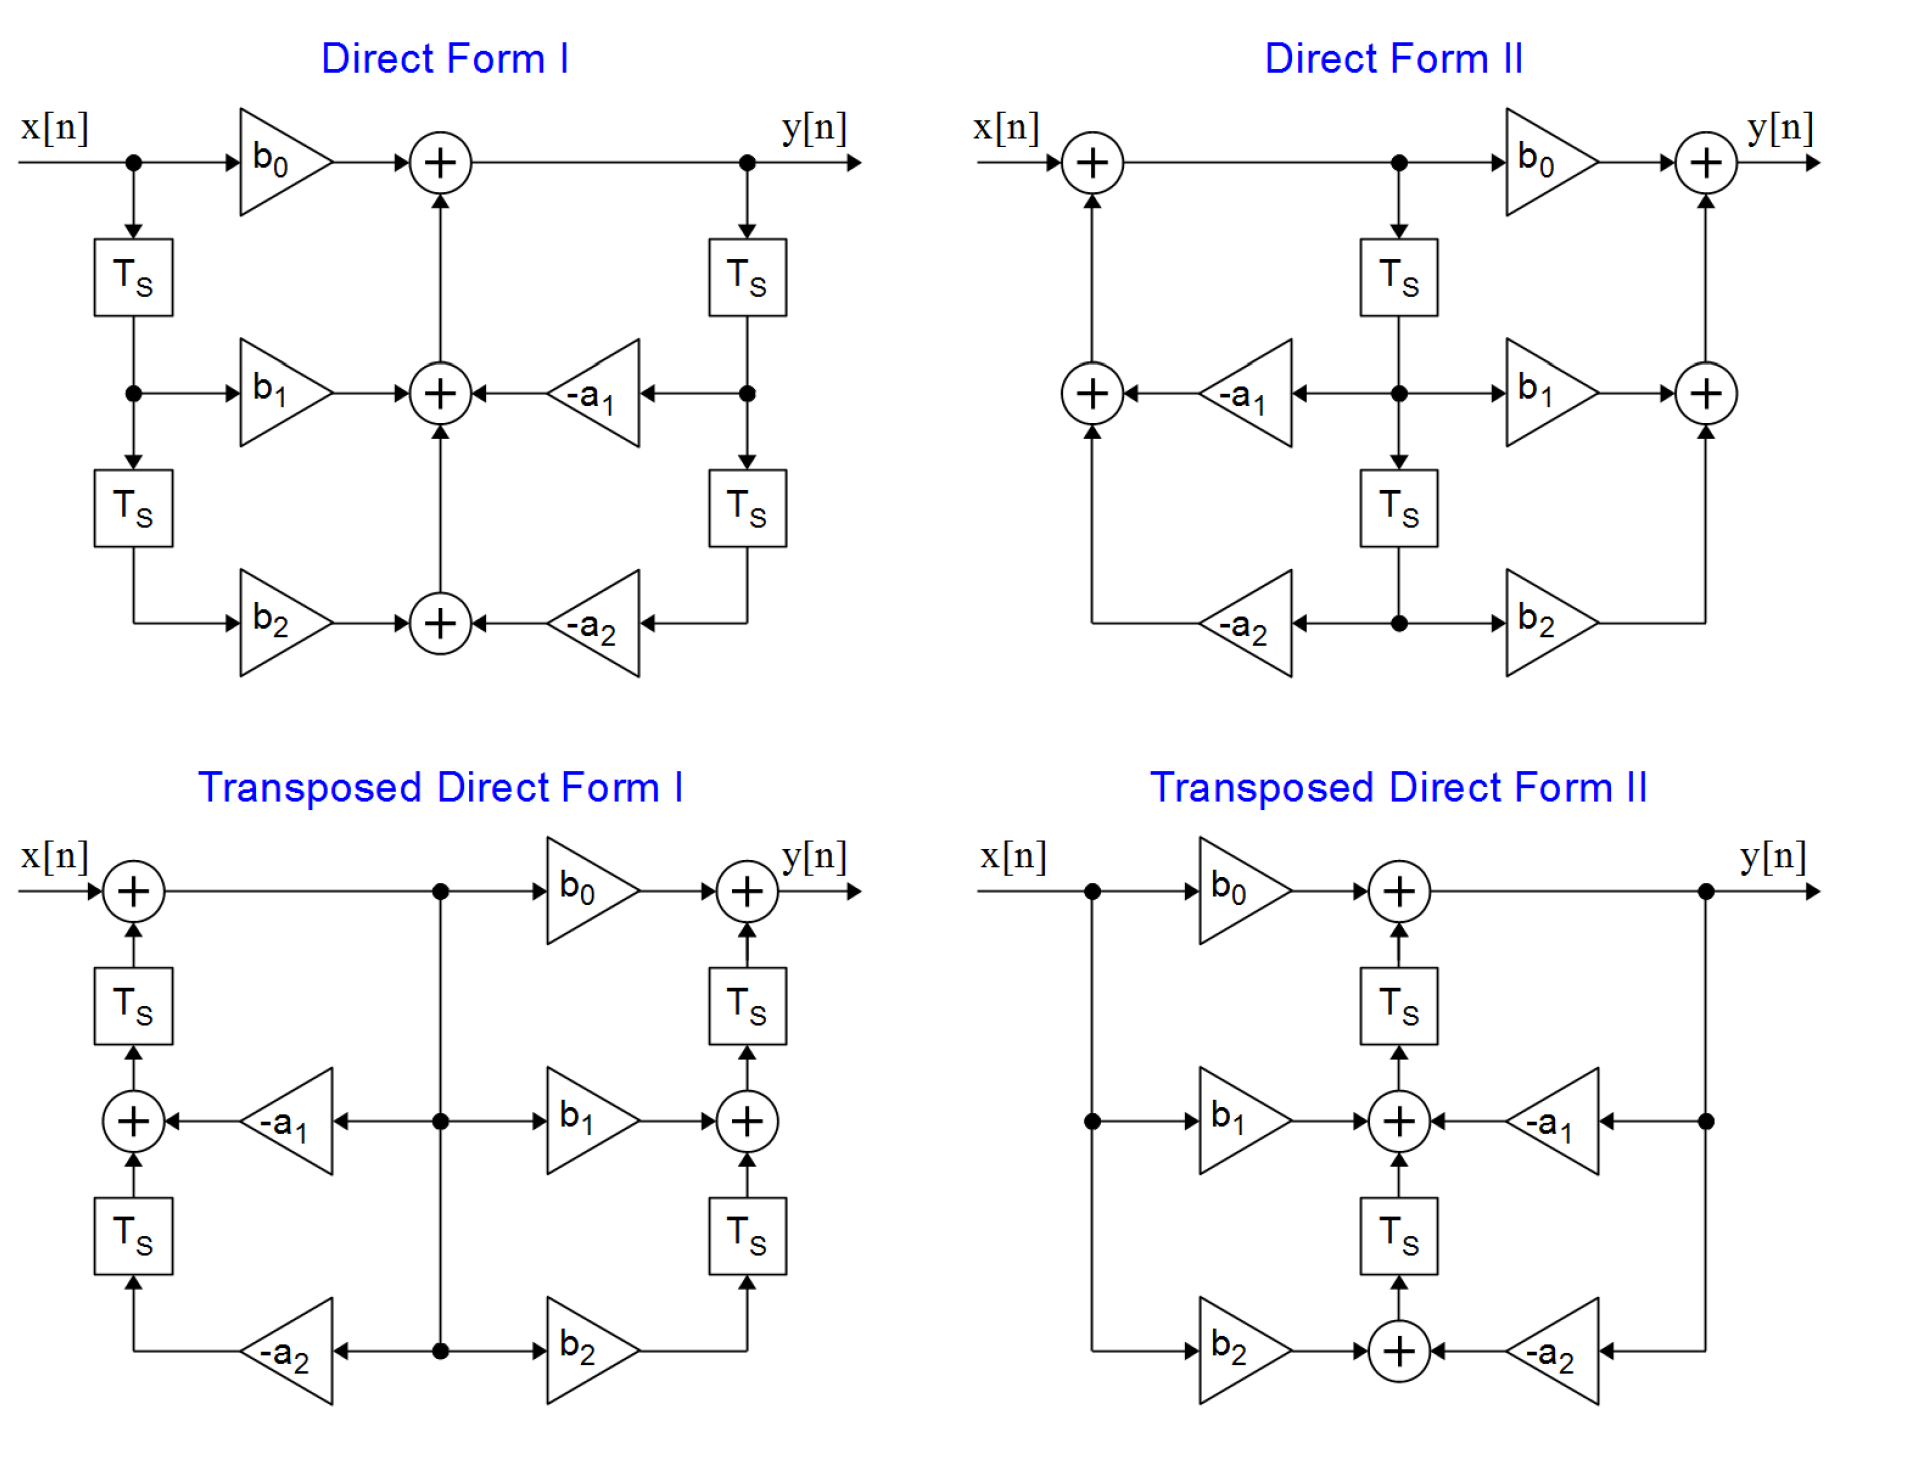
\includegraphics[width=.7\textwidth]{../fig/lti_scheme}
\end{center}

%===============================================================================
\section{Übertragungsfunktion}
Differenzengleichung:
\[y[n] = \sum_{k=0}^{N}b_k \cdot x[n-k]-\sum_{k=0}^{M} a_k \cdot y[n-k]\]
Übertragungsfunktion ($a_0$ normiert auf 1):
\[ H(z) = \frac{Y(z)}{X(z)} =
\frac{b_0+b_1 \cdot z^{-1} + b_2 \cdot z^{-2}+\ldots+b_N \cdot z^{-N}}
	{1+a_1 \cdot z^{-1} + a_2 \cdot z^{-2}+\ldots+a_M \cdot z^{-M}} \]
Amplituden, Phasengang:
\[ H(\Omega)=H(z)\big|_{z=e^{j\Omega}} \]
Beim Amplitudengang wird der Betrag $\big| H(\Omega)\big|$ in Abhängigkeit von $\Omega$ geplottet:\\
\[ \big| H(\Omega)\big| =  |K| \cdot \frac{|(z-z_1)||(z-z_2)|..|(z-z_N)|}
								{|(z-p_1)||(z-p_2)|..|(z-p_M)|}
								\cdot |z|^{M-N} \]
Phasengang: \[ \varphi(H(z)) = \sum_{k=1}^{N} \varphi(z-z_k) 
								-\sum_{k=1}^{M} \varphi(z-p_k)
								+\sum_{k=N+1}^{M} \varphi(z)  \]
Trick 1:
\[ 1-e^{-k \cdot jx} = e^{-\frac{k}{2} \cdot jx} \cdot (e^{\frac{k}{2} \cdot jx} - e^{-\frac{k}{2} \cdot jx})\]
Trick 2:
\[ sin(x)= \frac{e^{j \cdot x}-e^{-j \cdot x}}{2j} \hspace{20mm} 
cos(x)= \frac{e^{j \cdot x}+e^{-j \cdot x}}{2} \]
\textbf{Beispielaufgabe Phasenwinkel:\\} 
Analytisches Ermitteln des Phasenganges für die Übertragungsfunktion $H(z) = 1-z^{-4}$:
\begin{align*}
\angle H(\Omega)		 	&=\angle H(z)\big|_{z=e^{j\Omega}} \\
											&=\angle (1-e^{-4 \cdot j\Omega}) \\
\text{Anwenden von Trick 1:} 		&= \angle(e^{-2 \cdot j\Omega} \cdot (e^{2 \cdot j\Omega} - e^{-2 \cdot j\Omega})) \\
\text{Anwenden von Trick 2:} 		&= \angle(\underbrace{e^{-2 \cdot j\Omega}}_{= -2\Omega} 
\cdot \underbrace{2 \cdot j}_{+\frac{\pi}{2}} \cdot \underbrace{sin(2\Omega)}_{
\substack{ {0    \text{ für: } 0\leq \Omega \leq \frac{\pi}{2}} \\ 
           {+\pi \text{ für: } \frac{\pi}{2} \leq \Omega \leq \pi}}})
\end{align*}
Es gibt somit eine Fallunterscheidung für die zwei Bereiche von $\Omega$. Dies ist zuständig für den Phasensprung bei $\pi/2$. 
Graphische Darstellung des Phasenwinkels für das letzte Element (sinus):
\begin{center}
	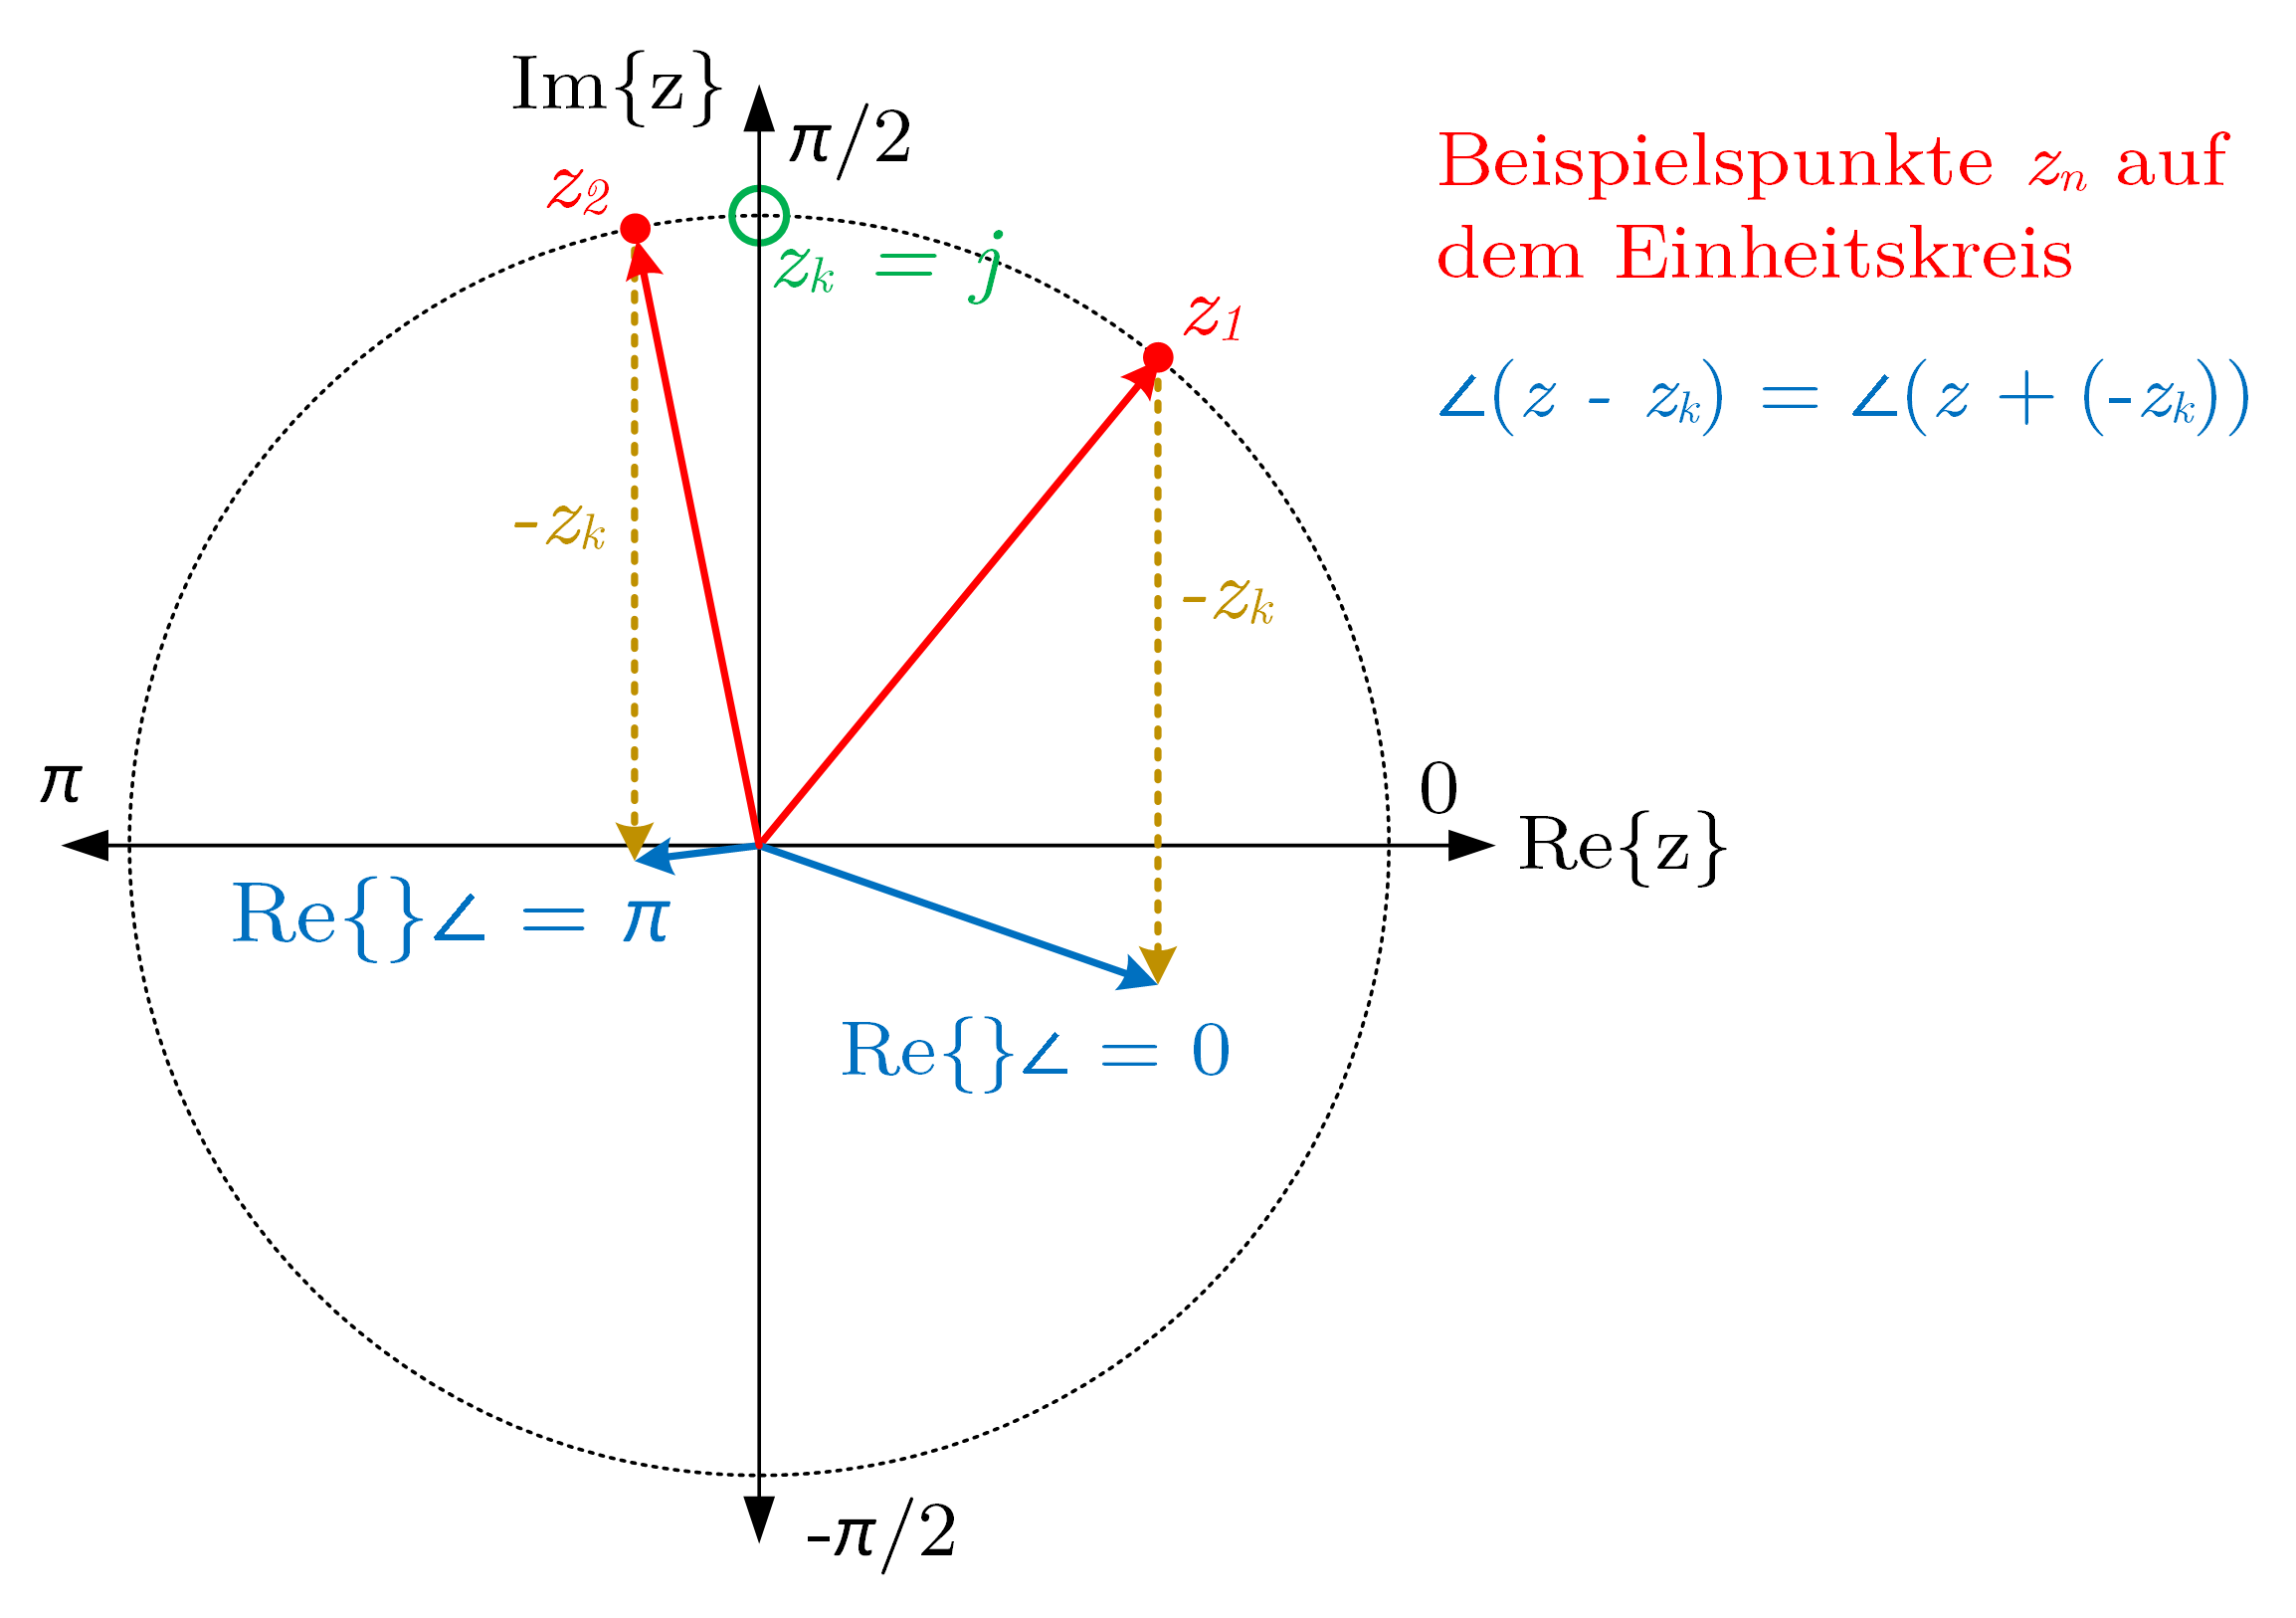
\includegraphics[width=.575\textwidth]{../fig/phasenwinkel_analyse}
\end{center}
\textbf{Beispielaufgabe Verstärkung:\\} 
Berechnen der Frequenz, bei der die Verstärkung $\big|H(z)\big|$ von $H(z) = 1-z^{-1} =\sqrt{2}$ ist:
\begin{align*}
 H(\Omega)	 	&= H(z)\big|_{z=e^{j\Omega}} \\
\big| H(\Omega)\big| &= \big|1-e^{-j\Omega}\big| = \frac{\big|e^{j\Omega}-1\big|}{\big|e^{j\Omega}\big|} 
          \Longrightarrow \big|e^{j\Omega}\big| \text{ aus dem Nenner} = 1 \\
\text{Verinfacht sich somit zu: }	\big| H(\Omega)\big| &= \big|e^{j\Omega}-1\big| \\
\text{Anwenden von Trick 1:} 		&= \big| e^{j\frac{\Omega}{2}} \cdot (e^{j\frac{\Omega}{2}} - e^{-j\frac{\Omega}{2}})\big| 
          \Longrightarrow \big|e^{j\frac{\Omega}{2}}\big| \text{ vor der Klammer} = 1\\
\text{Vereinfachen \& Anwenden von Trick 2:} &= \big| 2\cdot j \cdot sin\left(\frac{\Omega}{2}\right) \big| = 2 \cdot \big| sin\left(\frac{\Omega}{2}\right) \big| \stackrel{!}{=} \sqrt{2} \\
\text{Auflösen der Gleichung nach } \Omega \text{ ergibt: } \Omega_0 &= \frac{\pi}{2}, \Omega_1 = \frac{3}{2}\pi
\end{align*}
\newpage

%===============================================================================
\section{FIR (finite impulse response) Filter}
Bei einem FIR-Filter ist die Ordnung des Nenners immer $M=0$, die
Übertragungsfunktion für Ordnung $N$ lautet:
\[ H(z) =b_0 + b_1z^{-1} + \ldots + b_Nz^{-N} \]
Die Impulsantwort ist $N+1$ Zeitschritte lang und entspricht den Koeffizienten
von $H(z)$:
\[ h[n] = \{ b_0,b_1,\ldots,b_N,0,0,\ldots \} \]\\
\textbf{Stabilität:} 
Da alle Pole bei $z=0$ liegen, sind FIR-Filter per Definition stabil.\\
\textbf{Lineare Phase:} 
Mit einem FIR-Filter is es einfach möglich, eine lineare Phasenübertragung
zu realisieren.\\
\textbf{Implementation:}
Die Realisierung von FIR-Filtern in HW oder SW ist straightforward und unkritisch.

%===============================================================================
\subsection{Symmetrische FIR-Filter}
Ein FIR-Filter ist symmetrisch wenn:
\[ b_i = \pm b_{N-i} \qquad i = 0,1,\ldots,N \]
\begin{itemize}[noitemsep,topsep=3pt]
	\item Gespiegelt-symmetrischer (oder einfach symmetrischer) FIR-Filter: Gleichung mit "'+"' ist erfüllt.
	\item Anti-symmetrischer FIR-Filter: Gleichung mit "'-"' ist erfüllt.
\end{itemize}\vspace{5pt}
Alle symmetrischen Filter haben eine lineare Phasenantwort im Pass-Band und somit 
eine konstante Gruppenlaufzeit:
\[ \tau_g = \frac{N}{2} \cdot T_S \]
Beispiel für Filter mit Ordnung 6 (links) \& Ordnung 7 (rechts).
\begin{center}
	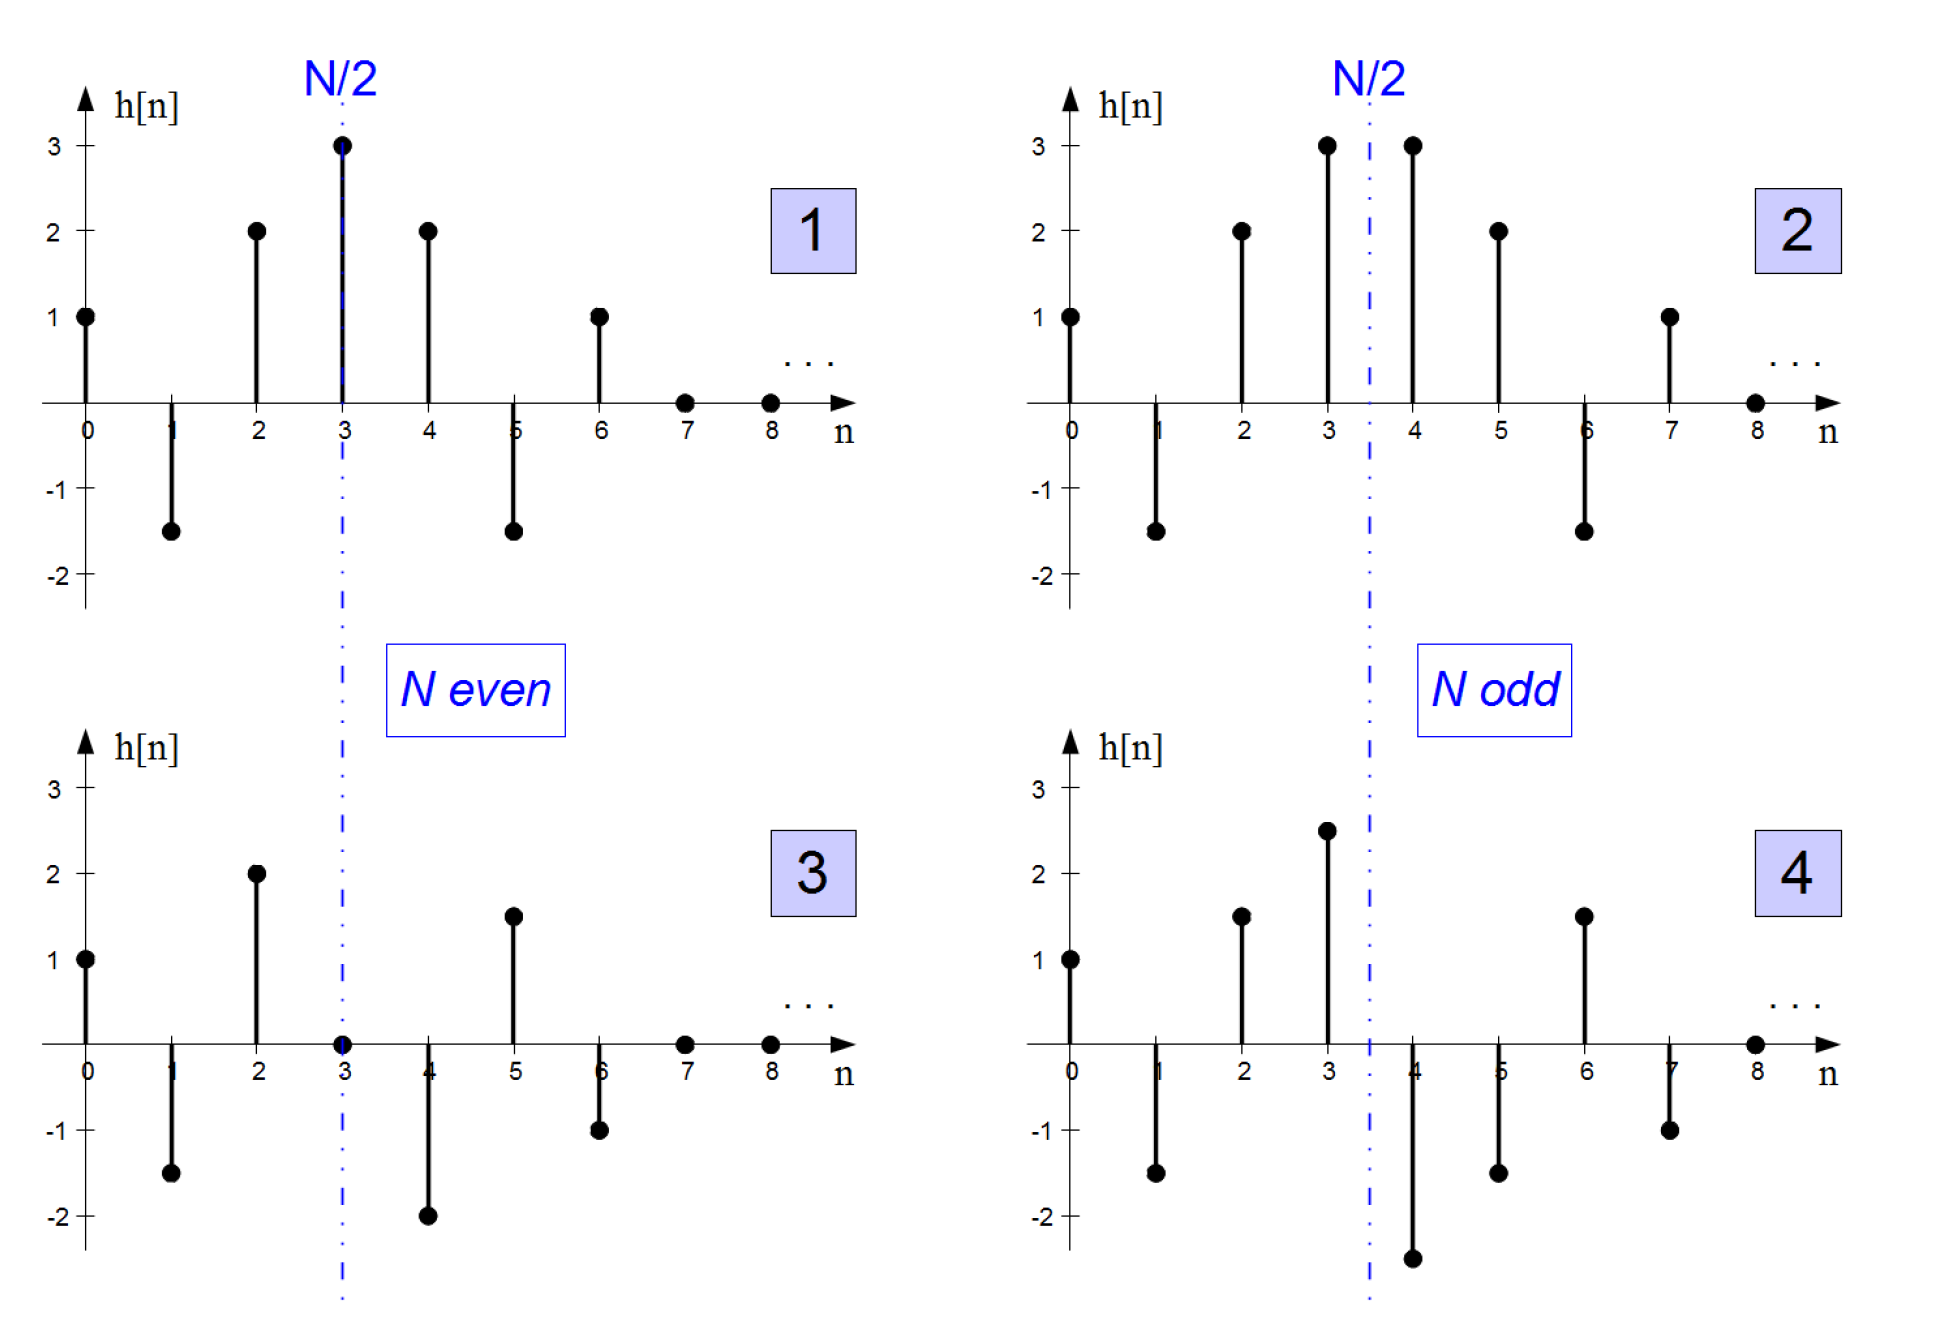
\includegraphics[width=.7\textwidth]{../fig/fir_filter}
	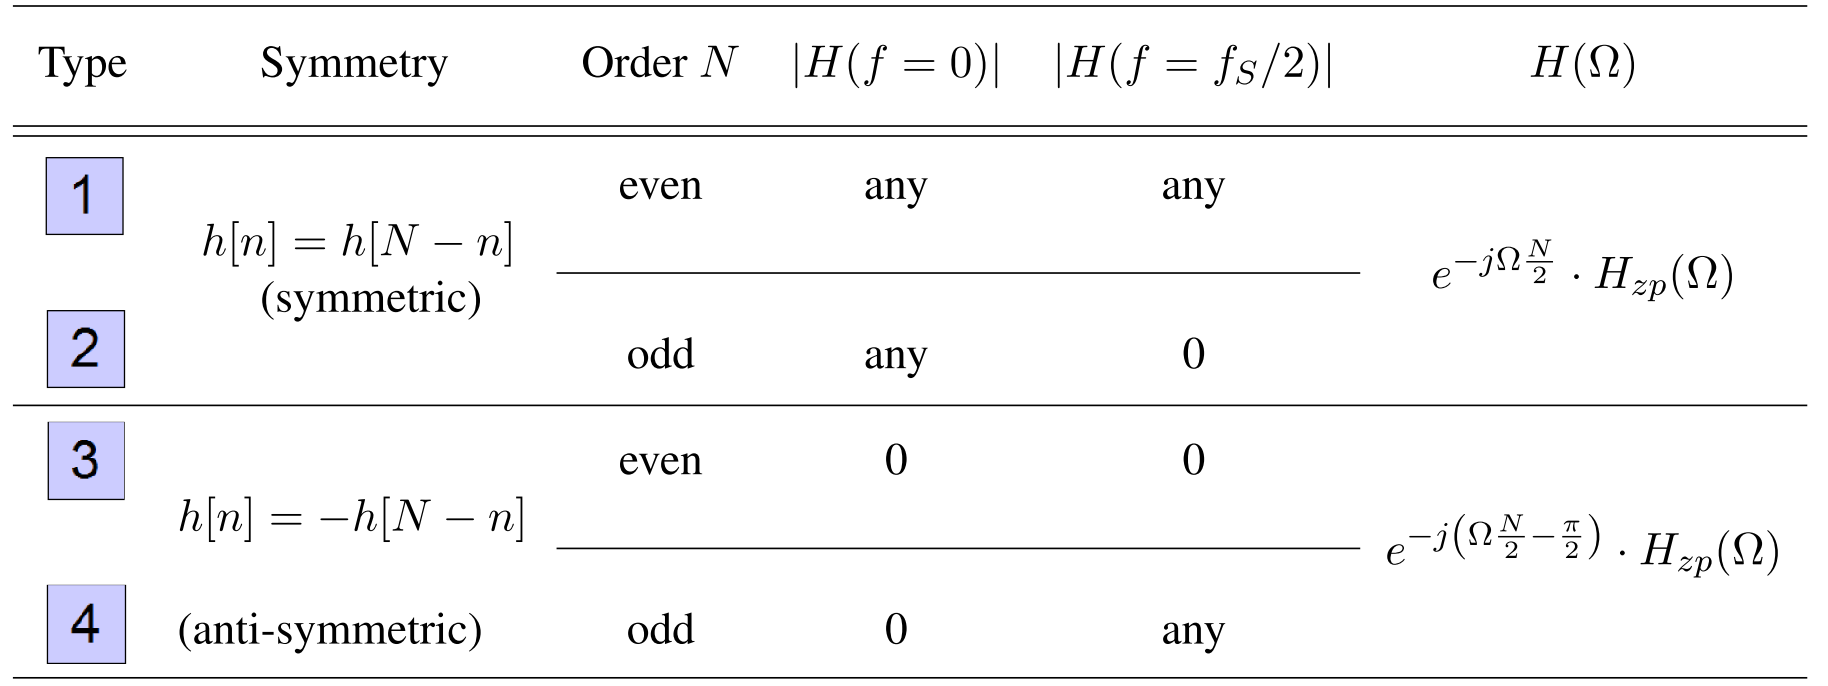
\includegraphics[width=.75\textwidth]{../fig/fir_table}
\end{center}
\textbf{Anmerkung Phasensprung \& Gegenmassnahme:\\}
Im Stop-Band symmetrischer FIR-Filter können 180\textdegree -Phasensprünge auftreten.
Sie entstehen bei jedem Frequenzpunkt von komplex-konjugierten Nullstellen am Einheitskreis.
Im Normalfall werden sie toleriert, da die Dämpfung im Stopp-Band entscheidend ist. 
Ansonsten können die Sprünge durch Duplikate der komplex-konjugierten Nullstellen-Paare 
eliminiert werden. Achtung: Dies erhöht jedoch die Gruppenlaufzeit durch die entstehende
höhere Ordnung.\\\\
\textbf{Anmerkung Gruppenlaufzeit:\\} 
Symmetrische FIR-Filter weisen eine lineare Gruppenlaufzeit auf mit $N/2$ Samples.
Die Nullstellen dieser Filter treten in reziproken Paaren auf (z.B. bei $-1/2$ und $-2$).
%===============================================================================
\subsection{Window Design Methode}
Der Matlab-Befehl \verb|fir1()| verwendet die Window Design Methode. Es wird mit 
der Impulsantwort eines idealen Tiefpass-Filters mit Cutoff-Frequency $f_c$ gestartet. 
Die ideale Impulsantwort ist nicht endlich. Sie wird auf eine endliche Länge von $N+1$ 
begrenzt und um $N/2$ Samples geshiftet. 
\[ h_{d_{TP}}[n]= \frac{sin(\Omega_c \cdot n)}{n \cdot \pi} \qquad \qquad
			\Omega_c = 2 \cdot \pi \cdot \frac{f_c}{f_S}, \text{ }n = \bigg\{\frac{-N}{2},...,\frac{N}{2} \bigg\} \]
Für den Wert von $h_{d_{TP}}[0]$ muss aufgrund der Nulldivision die Regeln von L'Hospital angewendet werden (normalisiert auf $f_S$!):
\[ 
	\frac{\text{d}}{\text{d}n}  \left( \frac{ sin(2\cdot f_c \cdot \pi \cdot n} {\pi \cdot n} \right)\bigg|_{n=0}= 
	\frac{2\cdot f_c \cdot \pi \cdot cos(2\cdot f_c \cdot \pi \cdot 0)}{\pi} = 2 \cdot f_c \qquad \qquad h_{d_{TP}}[0]= \frac{2 \cdot f_c}{f_S}
\]
\begin{enumerate}[noitemsep,topsep=3pt]
	\item Ideale Tiefpass Übertragungsfunktion
	\item Ideale Impulsantwort (nicht endlich)
	\item Begrenzen der Impulsantwort mittels Fenster
	\item Geshiftete Impulsantwort zur praktischen Umsetzung
\end{enumerate}
\begin{center}
	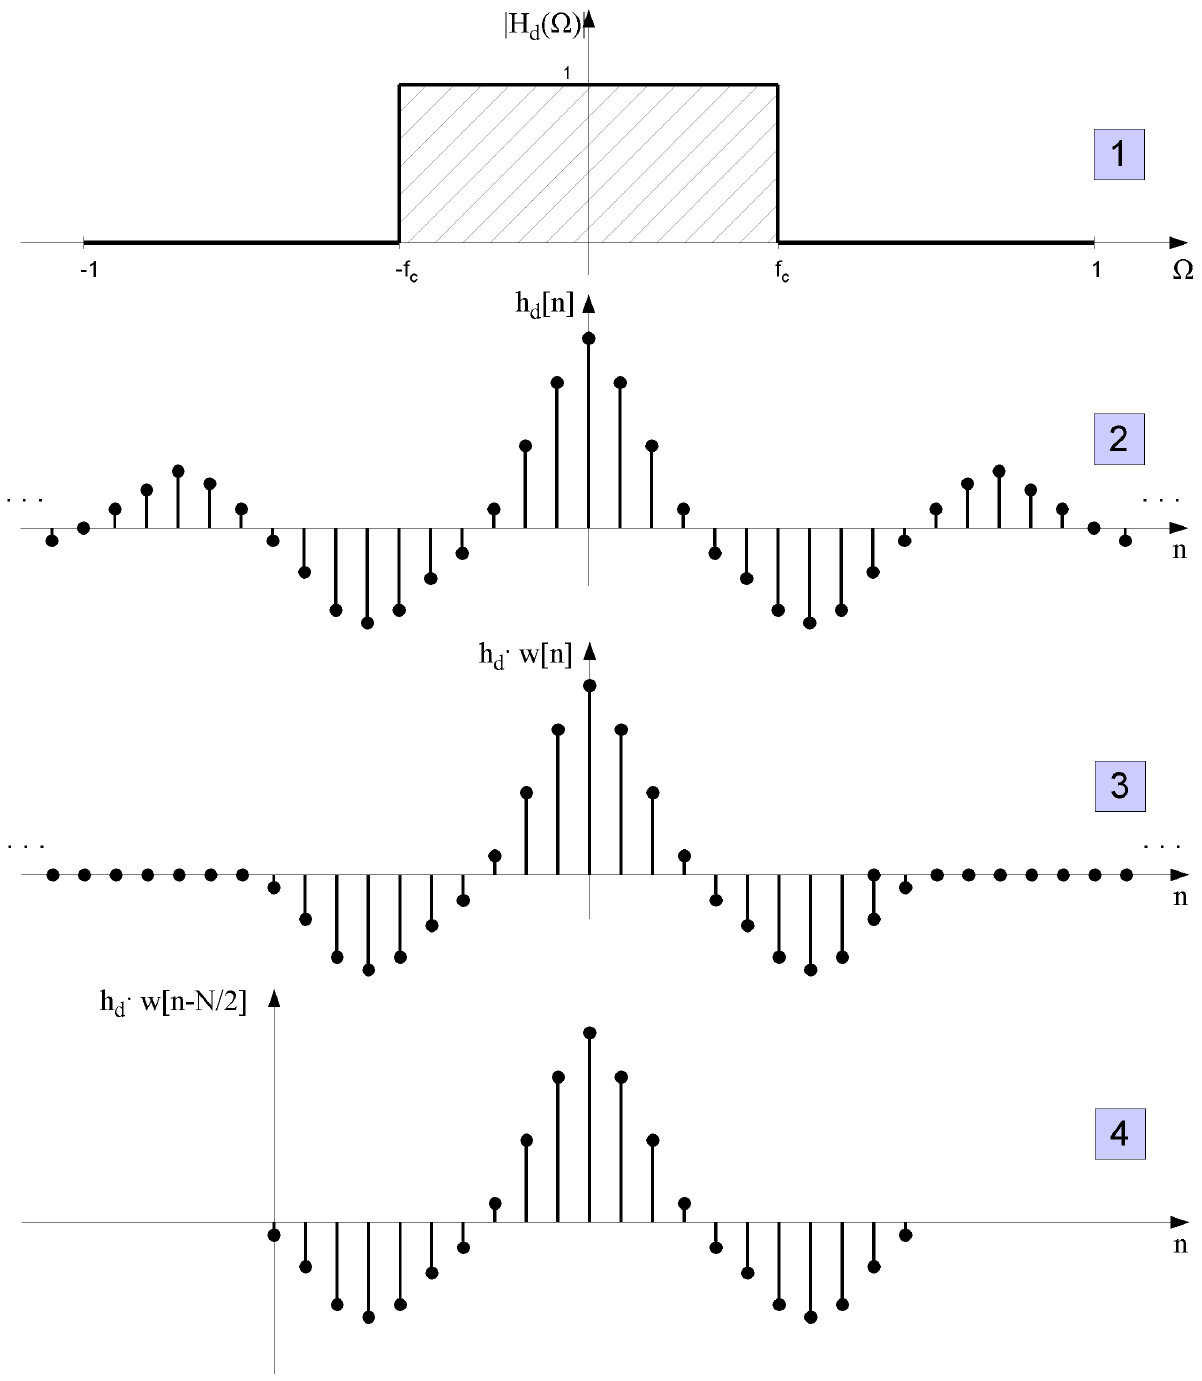
\includegraphics[width=.625\textwidth]{../fig/window_design_methode}
\end{center}
\textbf{Vorgehen für Band- und Hochpass:\\}
Band- und Hochpass-Filter werden durch die Summe oder Differenz von Tiefpass-Filtern
mit unterschiedlichen Cutoff-Frequencies bestimmt. Beispiel von Hochpass: Tiefpass mit 
$f_c = f_S/2$ minus ein anderer Tiefpass mit der $f_c$. Die Impulsantwort des 
Hochpassfilters lautet demnach:
\begin{align*}
	h_{d_{HP}}[n]&= \frac{sin(n \cdot \pi)}{n \cdot \pi} - \frac{sin(\Omega_c \cdot n)}{n \cdot \pi} 
	= -h_{d_{TP}}[n], \text{ wobei: } h_{d_{HP}}[0]= 1 - h_{d_{TP}}[0]  \\
	&=\{ ...,\ -h_{d_{TP}}[-2],\ -h_{d_{TP}}[-1],\ 1-h_{d_{TP}}[0],\ -h_{d_{TP}}[1],\ -h_{d_{TP}}[2],\ ... \} 
\end{align*}
\textbf{Zusammenhang zwischen Overshoot, Übergangsband, Ordnung \& Window-Typ:\\}
Das Anwenden des Windows entspricht einer Faltung des idealen Frequenzgangs mit
einem Rechteckfenster. Dadurch entsteht ein Overshoot bei den Übergängen der Bänder. 
Der Overshoot kann durch erhöhen von $N$ nicht reduziert werden, jedoch wird dadurch 
die Breite des Übergangsbereichs verringert. Um den Overshoot zu verringern, muss 
ein anderes Windows als das Rechteck eingesetzt werden. Das Übergangsband wird dadurch
jedoch etwas breiter.
%===============================================================================
\subsection{Alternative Designmethoden}
\textbf{Equiripple:} Erzielt teils tiefere Filter-Ordnung $N$ für dieselben Spezifikationen,
da der Rippel im Durchlass- und Stoppband gewichtet werden kann. Der Filter weisst dabei  
eine konstante Rippel-Amplitude auf.\\
\textbf{Frequenz-Sampling:} Man sampelt den idealen Frequenzgang $H_d(\Omega)$ an $N$ 
Sample-Punkten in identisch grossem Abstand. Durch Anwenden der IDFT zwischen 0 ... $2\pi$
erhält man die Impulsantwort.
%===============================================================================
\subsection{FIR-Kammfilter}
z-Übertragungsfunktion des Kammfilters $N$-ter Ordnung:
\[ H(z)\ =\ 1\ \pm z^{-N} \]
Impulsantwort:
\[ h[k]= [b_0 \ 0 \dots 0 \ b_N] =  [1 \ 0 \dots 0 \ \pm1] \]
Alle $N$ Pole sind im Ursprung. Die Nullstellen ergeben sich aus den Einheitswurzeln, 
bei $b_N=1$ haben diese noch eine Phasenverschiebung (siehe linker Fall unten).
\begin{center}
	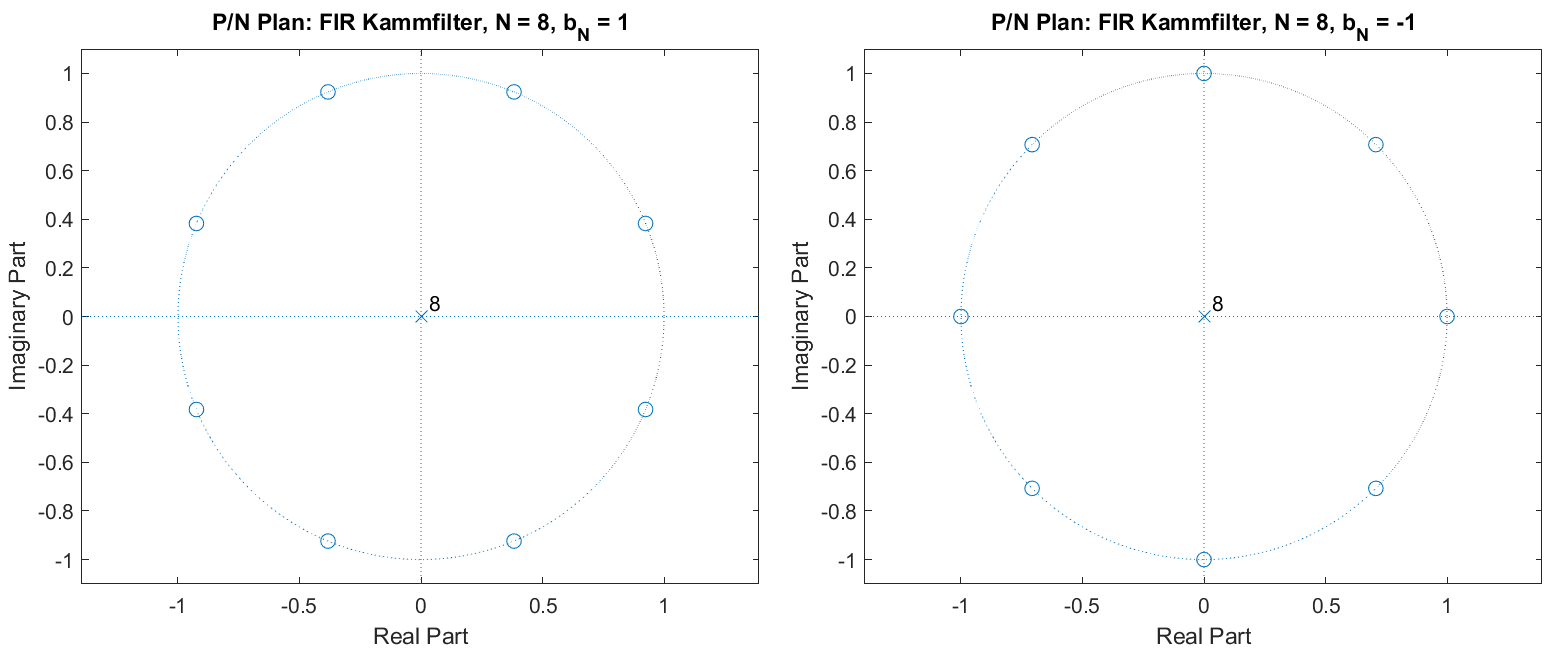
\includegraphics[width=0.875\textwidth]{../fig/fir_comb}
\end{center}\vspace{-4mm}
%===============================================================================
\subsection{Kanalausgleich mittels FIR}
Angenommen, ein Kanal verzerrt das Signal durch Echos. Die Impulsantwort ist endlich. 
Mittels Channel Equalization kann der Kanal entzerrt werden. Dazu eignet sich folgendes
Vorgehen, um die Koeffizienten des Filters in Echtzeit zu berechnen. Der Aufwand bezieht 
sich auf die Anzahl realer Multiplikationen (1 cpl Mul = 2 real Mul): 
\begin{enumerate}[noitemsep,topsep=3pt]
	\item FFT der Impulsantwort (Aufwand: $\left[\frac{N}{2}\cdot\log_2N\right]$)
	\item Invertierung aller Spektralwerte (Aufwand: $\left[N\right]$)
	\item IFFT des invertierten Spektrums (Aufwand: $\left[\frac{N}{2}\cdot\log_2N\right]$)
\end{enumerate}
Totaler Aufwand an realwertigen Multiplikationen: $2N + 2N\log_2N$
\newpage

%===============================================================================
\section{IIR-Filter}
\subsection{Eigenschaften}
Bei IIR-Filtern ist die Ordnung des Nenners $M>0$, es existieren also Polstellen bei 
$z\neq0$. Die Impulsantwort dieser Filter ist theoretisch unendlich. Generell kann mit 
einem IIR-Filter mit tieferer Ordnung derselbe Amplitudengang wie mit einem FIR-Filter 
erreicht werden. Die Laufzeit verkürzt sich dadurch, eine konstante Gruppenlaufzeit 
lässt sich jedoch nicht realisieren. Durch Quantisierungsfehler können IIR-Filter instabil 
werden. Tabellarischer Vergleich:
\begin{center}
	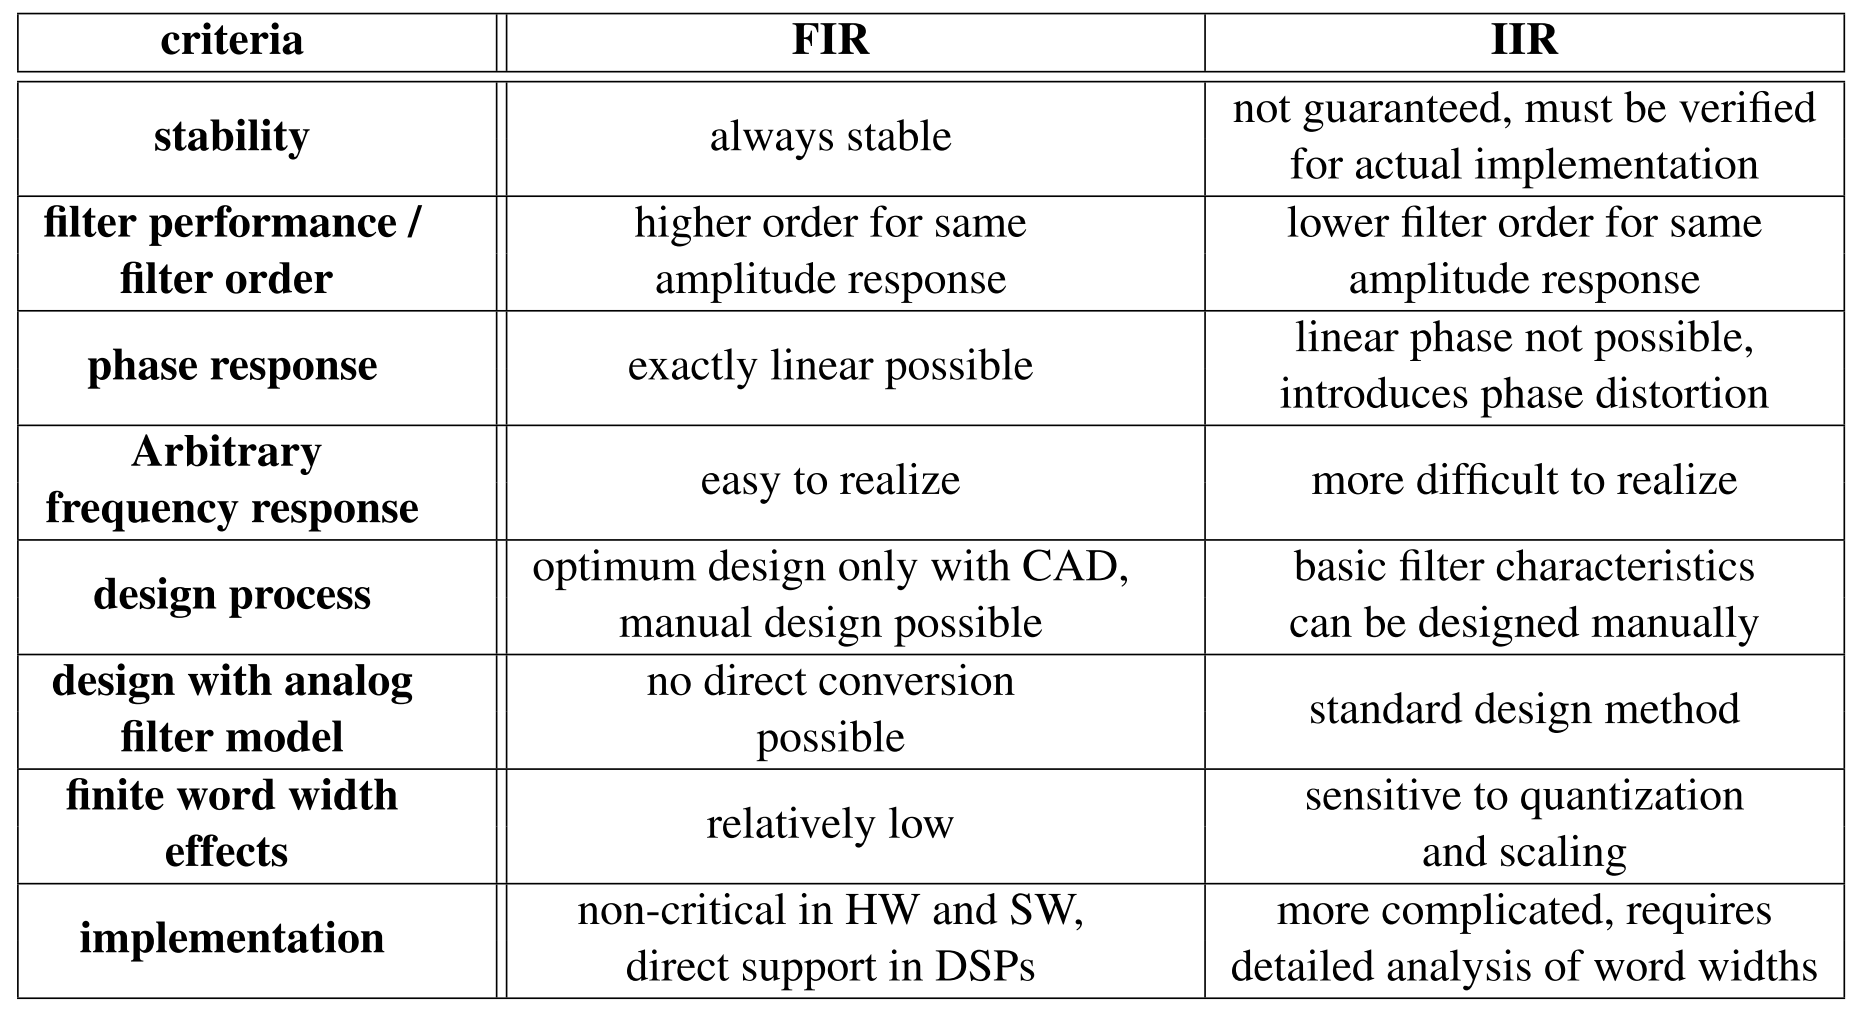
\includegraphics[width=.8\textwidth]{../fig/fir_vs_iir}
\end{center}
%===============================================================================
\subsection{IIR-Design mittels Impulsinvarianz-Transformation (Tiefpass)}
Die Impulsantwort des digitalen IIR-Filters wird durch Sampling der Impulsantwort des
analogen Prototyp-Filters ermittelt. Um Aliasing zu verhindern, muss $f_S$ mindestens doppelt so gross wie die höchste 
Durchlass-Frequenz des analogen Prototypen-Filters sein. Die Methode ist demnach nur 
für Tiefpass, jedoch nicht für andere Filter geeignet.
\[ h[n] = h_a(n \cdot T_S) \qquad n=0,1,2,... \]
Umformung von der $p$-Ebene zur $z$-Ebene:
\[ z = \e^{pT_S} \]
\begin{center}
	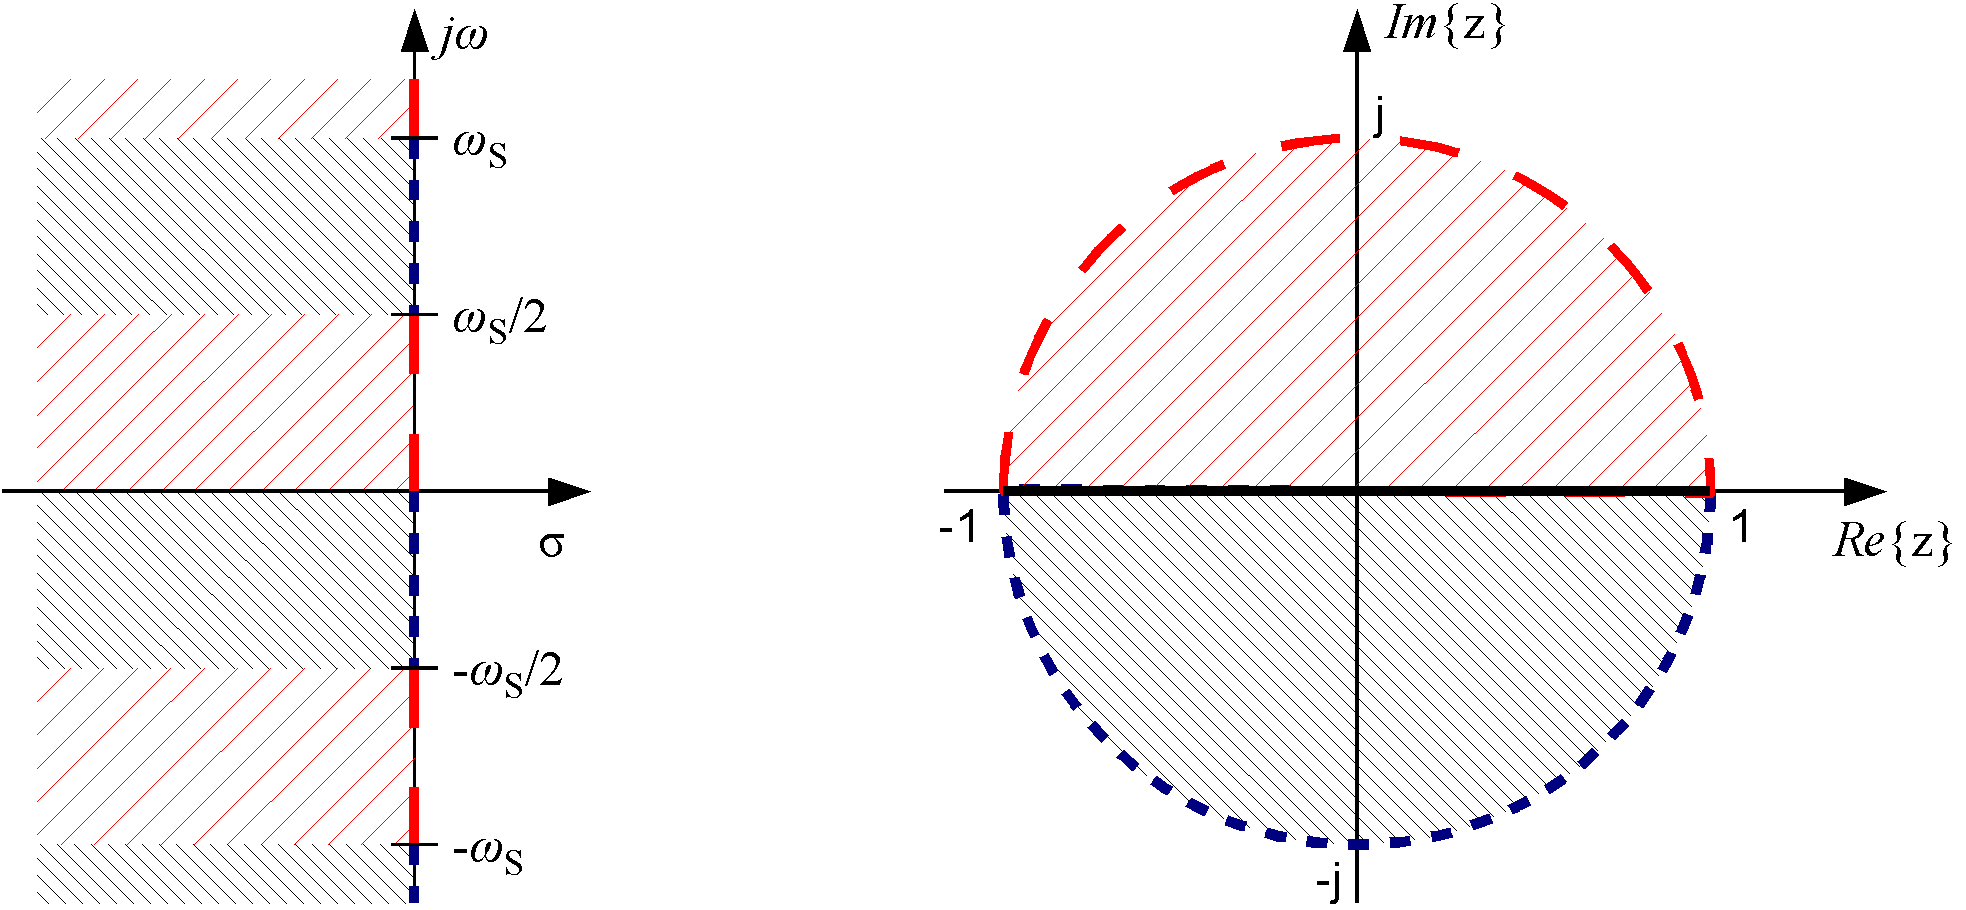
\includegraphics[width=.7\textwidth]{../fig/mapping_p_to_z_plane}
\end{center}
\newpage

%===============================================================================
\section{Implementationsaspekte}
Die Wahl der Sampling-Frequenz muss gut durchdacht sein. Bei zu hoher Sampling Frequenz entstehen Probleme:
\begin{itemize}[noitemsep,topsep=3pt]
	\item Grösserer Rechenaufwand, da mehr Samples in vorgegebener Zeit bearbeitet werden müssen.
	\item Je kleiner der Frequenzabstand zwischen Pass- und Stoppband wird, desto steiler wird die Filterkurve. 
	Dies wiederum erzwingt eine höhere Ordnung, was erneut den Rechenaufwand erhöht.
	\item Je näher Pol- und Nullstellen der Transferfunktion in der $z$-Ebene kommen, desto höher die Sensitivität 
	gegenüber Quantisierungseffekten der Koeffizienten. 
\end{itemize}
%===============================================================================
\subsection{Implementation von IIR-Filtern}
Der IIR-Filter kann als eine Kette von "'biquads"' implementiert werden. Dabei wird die
Übertragungsfunktion in $L$ Bläcke aufgeteilt, welche jeweils einen konjugiert-
komplexen Pol haben:
\[ H(z) = K \cdot \frac{(z-z_1)(z-z_1^*)}{(z-p_1)(z-p_1^*)}\cdot\ldots\cdot
	\frac{(z-z_L)(z-z_L^*)}{(z-p_L)(z-p_L^*)} \]
Die Sub-Übertragungsfunktionen werden dabei in der "'Direct Form I"' oder in der "'Transposed 
Direct Form I"' implementiert. Beispiel mit biquads zweiter Ordnung in der "'Transposed Direct 
Form II"':
\begin{center}
	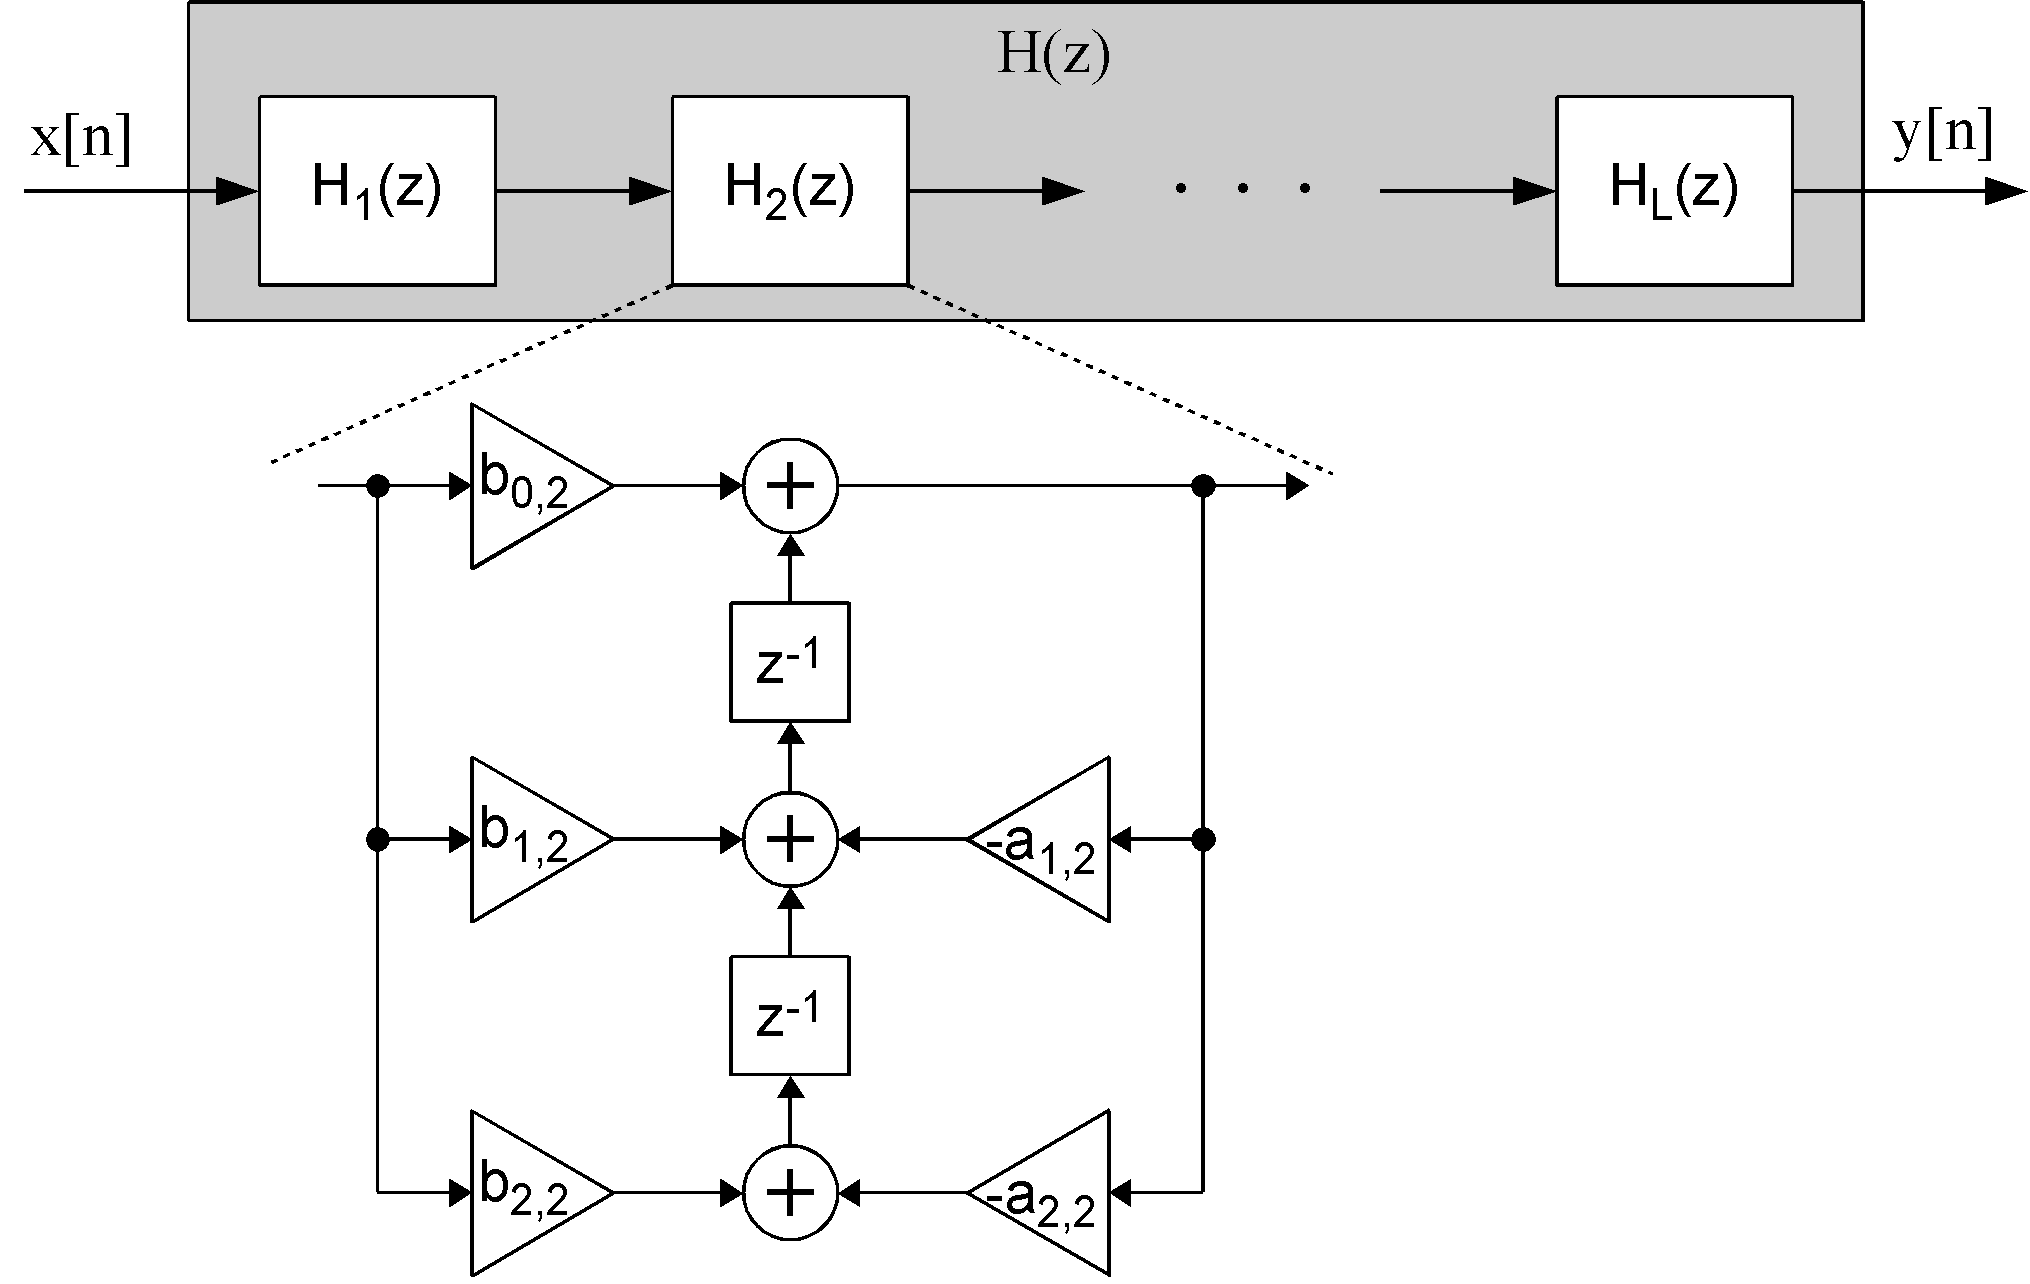
\includegraphics[width=.65\textwidth]{../fig/iir_implementation_biquads}
\end{center}
Matlab-Befehl zur Umwandlung der Koeffizienten von $H(z)$ in die Koeffizienten von $H_1(z), ..., H_L(z)$: \verb|tf2sos()|
\subsection{Fixkomma-Implementation}
Die Implementation im Fixkomma-Format ist resourceneffizienter als das Fliesskomma-Format.
Bei einer Fix-Point Implementierung mit $W$ Bits ($b_k$) und $F$ Nachkommastellen ist
der dezimale Wert:
\[ D_{ufix} = \sum_{k=0}^{W-1}b_k \cdot 2^{k-F} \]
Für Zahlen im Zweierkomplement ergibt sich der dezimale Wert wie folgt:
\[ D_{sfix} = -b_{W-1} \cdot 2^{W-F-1} + \sum_{k=0}^{W-2} b_k \cdot 2^{k-F} \]
\textbf{Overflow:}
Kann durch Hinzufügen zusätzlicher MSBs, einer Sättigung (Begrenzen der Zahlen auf grösste 
repräsentierbare Zahl) oder "'wrap-around"' (zählt beim kleinsten Wert weiter) erreicht werden.\\\\ 
\textbf{Underflow:}
Das Resultat kann aufgrund fehlender LSBs (Auflösung) nicht angezeigt werden. Zu den 
Massnahmen zählen Abschneiden (LSBs vernachlässigen) oder Runden (auf die nächst gelegene repräsentierbare Zahl).
% coding:utf-8

%----------------------------------------
%FOSADSVB, a LaTeX-Code for a summary of digital signal processing
%Copyright (C) 2015, Mario Felder & Michi Fallegger

%This program is free software; you can redistribute it and/or
%modify it under the terms of the GNU General Public License
%as published by the Free Software Foundation; either version 2
%of the License, or (at your option) any later version.

%This program is distributed in the hope that it will be useful,
%but WITHOUT ANY WARRANTY; without even the implied warranty of
%MERCHANTABILITY or FITNESS FOR A PARTICULAR PURPOSE.  See the
%GNU General Public License for more details.
%----------------------------------------

\chapter{Multirate und Filterbänke}
\section{Downsampling/Decimation}
Um ein Signal donwzusamplen, wird einfach nur jedes $D$-te Sample verwendet.
\begin{center}
	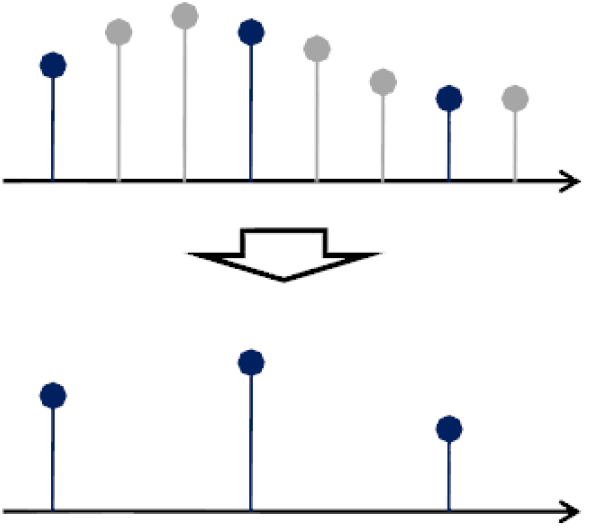
\includegraphics[width=.2\textwidth]{../fig/downsample}
	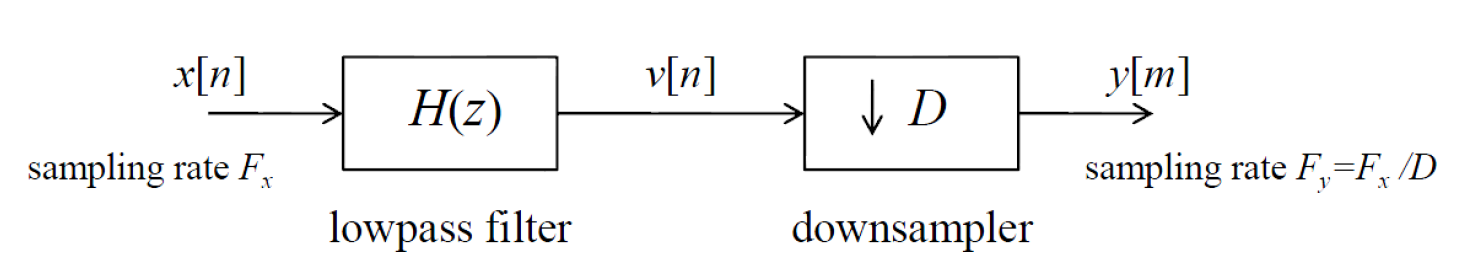
\includegraphics[width=.6\textwidth]{../fig/decimation}
\end{center}
Dabei muss beachtet werden, dass das Abtasttheorem noch eingehalten wird. Das
Signal muss zuerst mit einem Tiefpass gefiltert werden. Die Frequenzantwort des TP ist
idealerweise:
\[ H(\Omega) = \left\lbrace \begin{matrix}
	1 & \textrm{if } \Omega \in [-\pi/D,\pi/D]\\
	0 & \textrm{otherwise}
\end{matrix} \right. \] 
Das Resultat kann beschrieben werden als $y[m] = v[nD]$. Das Frequenzspektrum
wird um den Faktor $D$ horizontal gespreizt und gleichzeitig vertikal 
gestaucht. Für einen \emph{idealen} TP-Filter gilt für das resultierende Spektrum $Y(\Omega)$:
\[ Y(\Omega) = \frac{1}{D} V(\Omega/D)  \]
Allgemein für alle TP-Filter, wobei $d=1,...,D-1$ Aliasing aufgrund nicht idealer TP-Filterung einbezieht:
\[ Y(\Omega) = \frac{1}{D} \sum_{d=0}^{D-1} V(\Omega/D-2\pi d/D) \]
\begin{center}
	\includegraphics[width=.45\textwidth]{../fig/decimation_frequenz}
\end{center}
Als TP-Filter kann ein FIR Filter verwendet werden. Eine direkte Implementierung
ist nicht effektiv, da $D-1$ vom Filter berechnete Werte vom Downsampler
weggeworfen werden. Mit dem Downsampler vor dem Filter müssen weniger
Berechnungen durchgeführt werden. Die Multiplikatoren können mit einer 
tieferen Samplingrate betrieben werden. \\\\
Direkte, ineffiziente Implementation (links) \& effizientere Implementation (rechts):
\begin{center}
	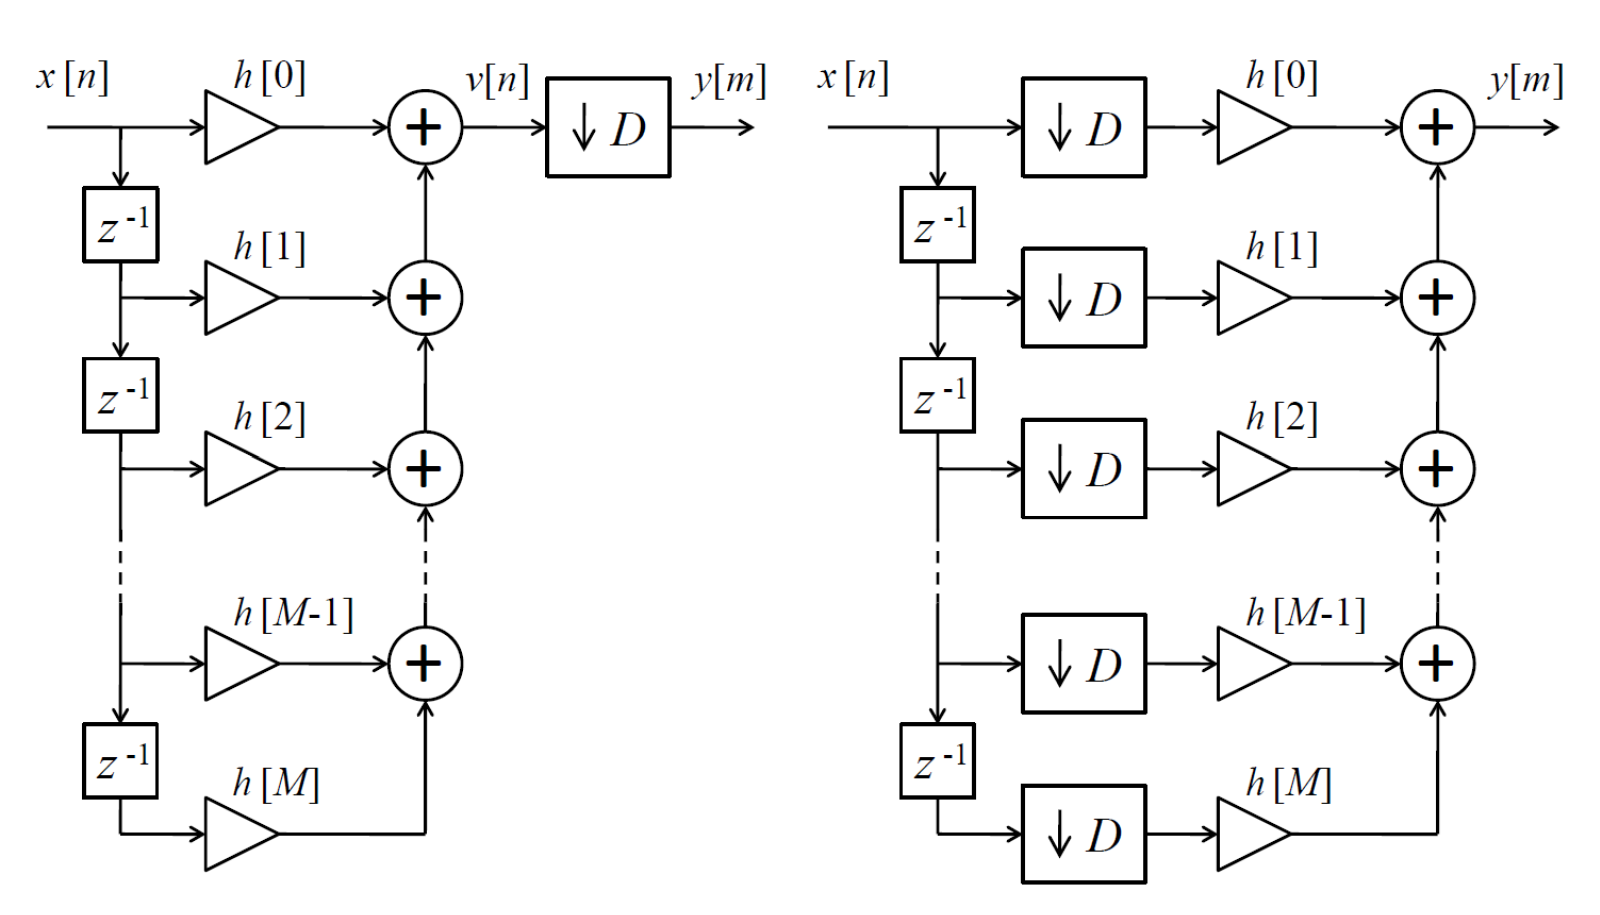
\includegraphics[width=.7\textwidth]{../fig/decimation_scheme}
\end{center}

%===============================================================================
\section{Upsampling/Interpolation}
Bei einem Upsampler mit dem Faktor $I$ werden zwischen zwei Samples jeweils
$I-1$ Nullen eingefügt.
\begin{center}
	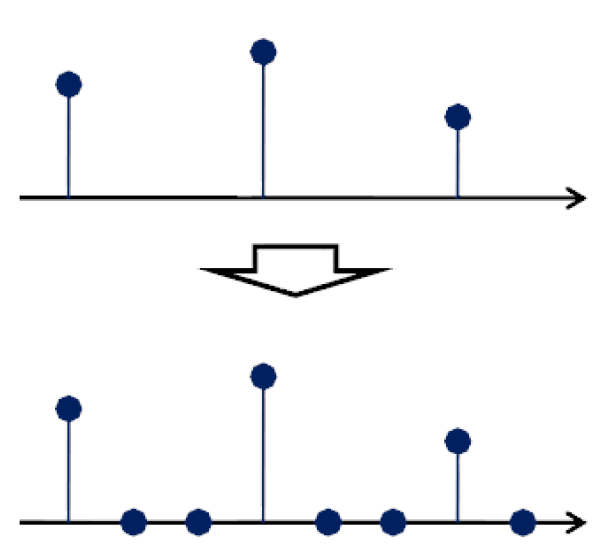
\includegraphics[width=.2\textwidth]{../fig/upsample}
	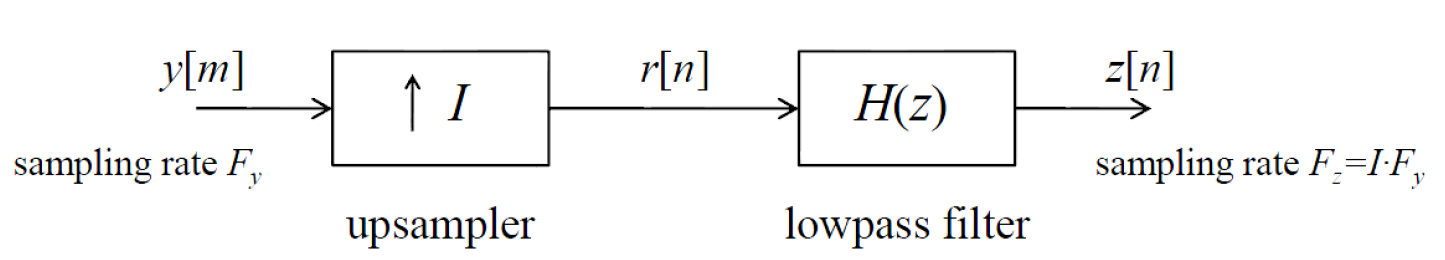
\includegraphics[width=.6\textwidth]{../fig/interpolation}
\end{center}
\[ r[n] = \left\lbrace \begin{matrix}
	y[n/I] & \textrm{if } n \in [0,\pm I, \pm 2I,\ldots]\\
	0 & \textrm{otherwise}
\end{matrix} \right. \] 
Die Abtastfrequenz $F_z$ ist $I$-mal höher als die Abtastfrequenz $F_y$ von
$y[m]$. Das Spektrum des upgesampelten Signal ist:
\[ \ R(\Omega) = \sum_{n=-\infty}^{\infty} r[n]
	\e^{-\im\Omega n} 
	= \sum_{m=-\infty}^{\infty} r[m]\e^{-\im\Omega m}
	= Y(I\Omega)  \]
Damit das Frequenzspektrum von $y[m]$ nicht periodisch mit der Periode
von $2\pi/I$ ist, ist eine Tiefpassfilterung nach dem Upsampling notwendig. 
Er glättet das Signal und führt dadurch die Interpolation durch. Der
ideale TP-Filter hat die Frequenzantwort:
\[ H(\Omega) = \left\lbrace \begin{matrix}
	I & \textrm{if } \Omega \in [-\pi/I,\pi/I]\\
	0 & \textrm{otherwise}
	\end{matrix} \right. \]

\begin{center}
	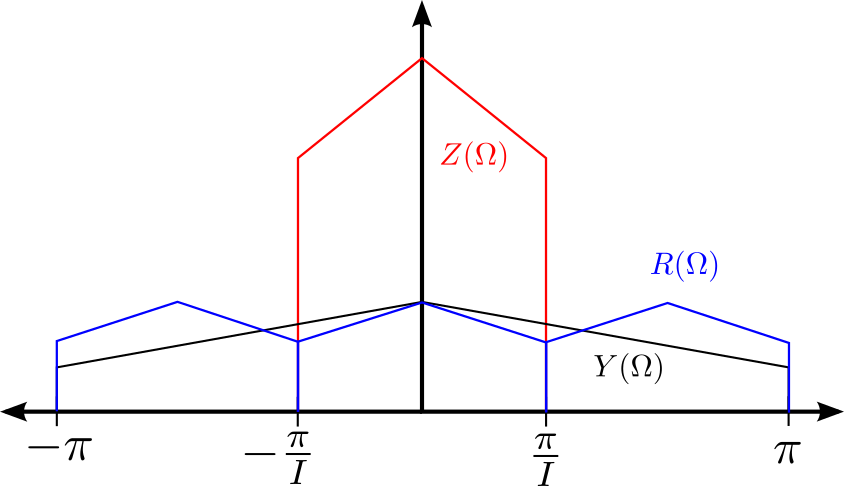
\includegraphics[width=.45\textwidth]{../fig/interpolation_frequenz.png}
\end{center}
Ein FIR oder IIR Filter kann als TP-Filter verwendet werden. Eine direkte
Implementierung (siehe linkes Blockschaltbild) ist ineffektiv, da der 
Filter auch auf die Null-Werte angewandt wird. Rechts muss der Multiplikator
nur mit der Frequenz $F_y$ arbeiten, im Vergleich zu links mit der höheren $F_z$
nach dem Upsampling.
\begin{center}
	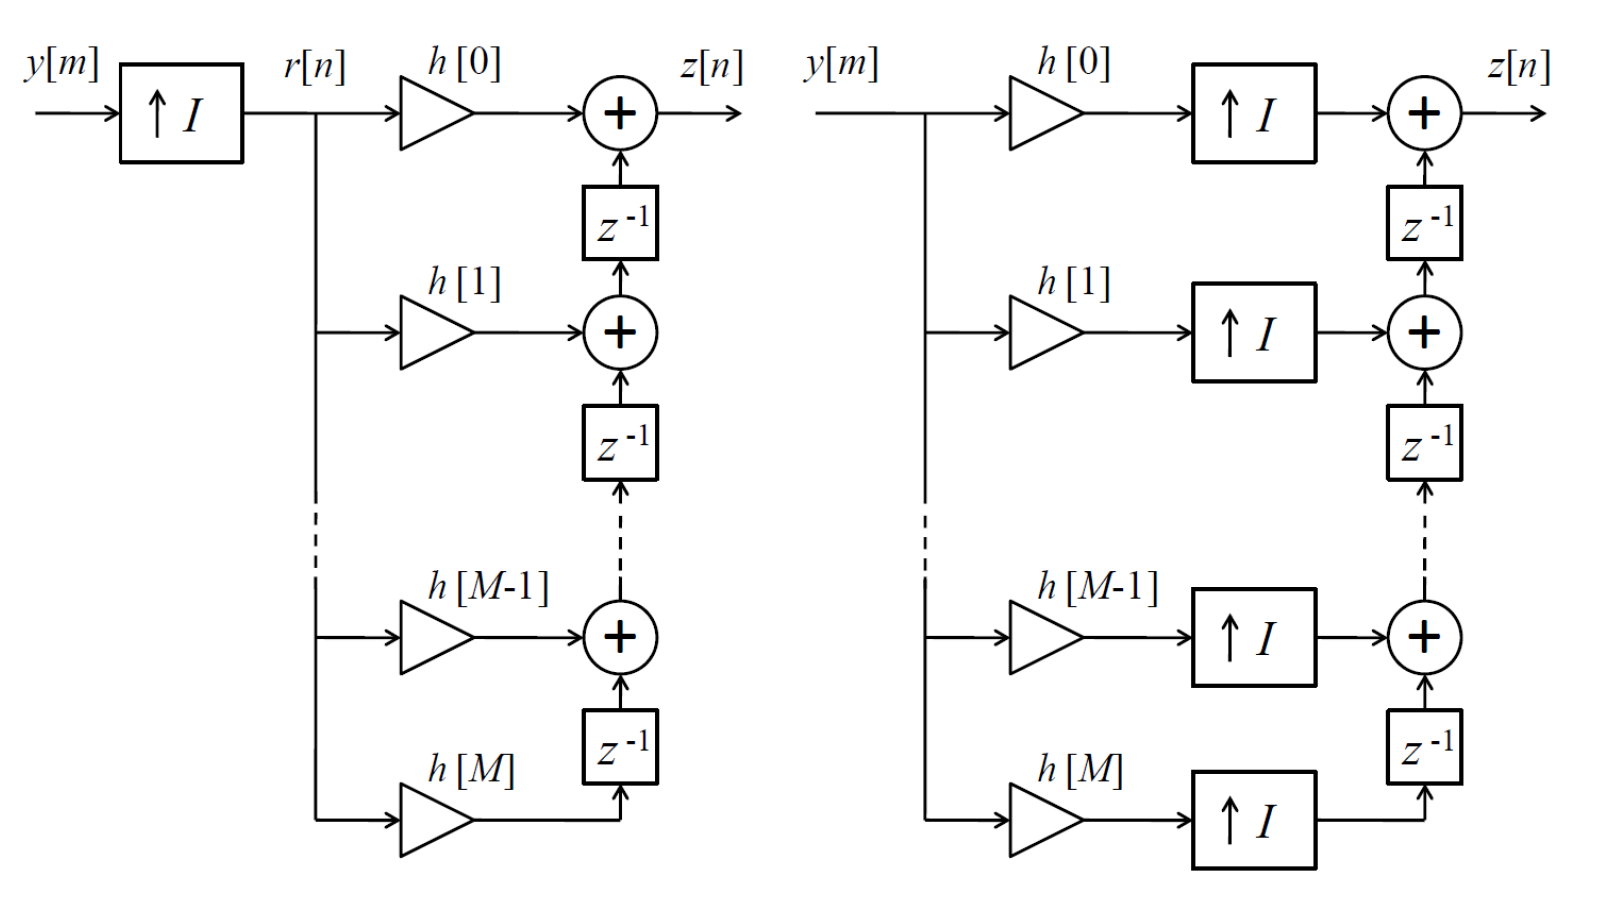
\includegraphics[width=.7\textwidth]{../fig/interpolation_scheme}
\end{center}

%===============================================================================
\section{Polyphasen Filter}
Dienen zur effizienteren Implementation von Filtern. 
Jede $i$-te Komponente von $p_i[k]$ beinhaltet den $M$-ten Koeffizienten der 
Impulsantwort $h[k]$, alle zusammen beinhalten die gesamten Informationen.
Insgesamt existieren also immer $M$ Polyphasenfilter.   
Die um $M$ downgesampelte Impulsantwort $h[k]$ ist definiert als:
\[ p_i[k] = h[kM+i] \qquad i=0,1,\ldots,M-1 \]
Dazugehörende z-Transformation für die Polyphasen-Komponenten $P_i(z)$:
\[ P_i(z) = \sum_{k=-\infty}^{\infty} p_i[k]z^{-k} \qquad i=0,1,\ldots,M-1 \]
Somit gilt für das Spektrum:
\[ H(z) = \sum_{i=0}^{M-1}z^{-i} P_i(z^M) \]
Der Vorteil liegt darin, dass die Filter bei einem Upsampling mit der Rate $F_y$ statt der höheren
Rate $F_z$ arbeiten können. Die einzelnen Werte müssen anschliessend nur noch
mit der $F_z=I \cdot F_y$ zusammengesetzt werden.\\
Bei einem Downsampling können die Filter mit $F_x/D$ arbeiten, während die Werte mit $F_x$ 
auf die einzelnen Polyphasen-Komponenten aufgeteilt werden. \\\\
\begin{minipage}{.48\textwidth}
	\centering
	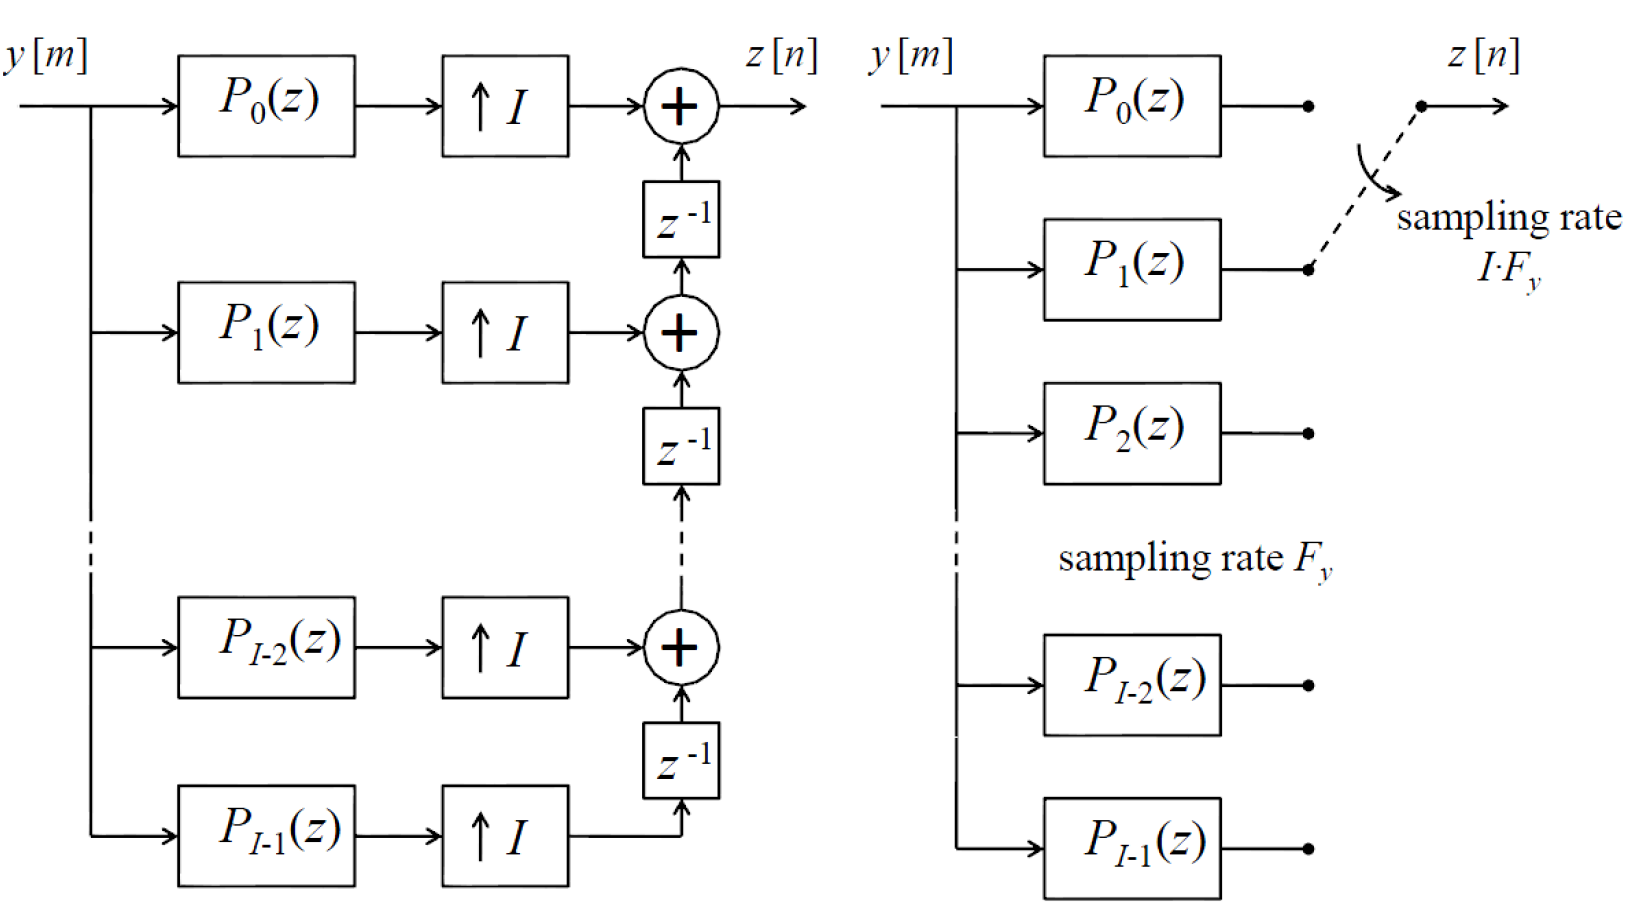
\includegraphics[width=\textwidth]{../fig/polyphase_up}
\end{minipage}
\begin{minipage}{.48\textwidth}
	\centering
	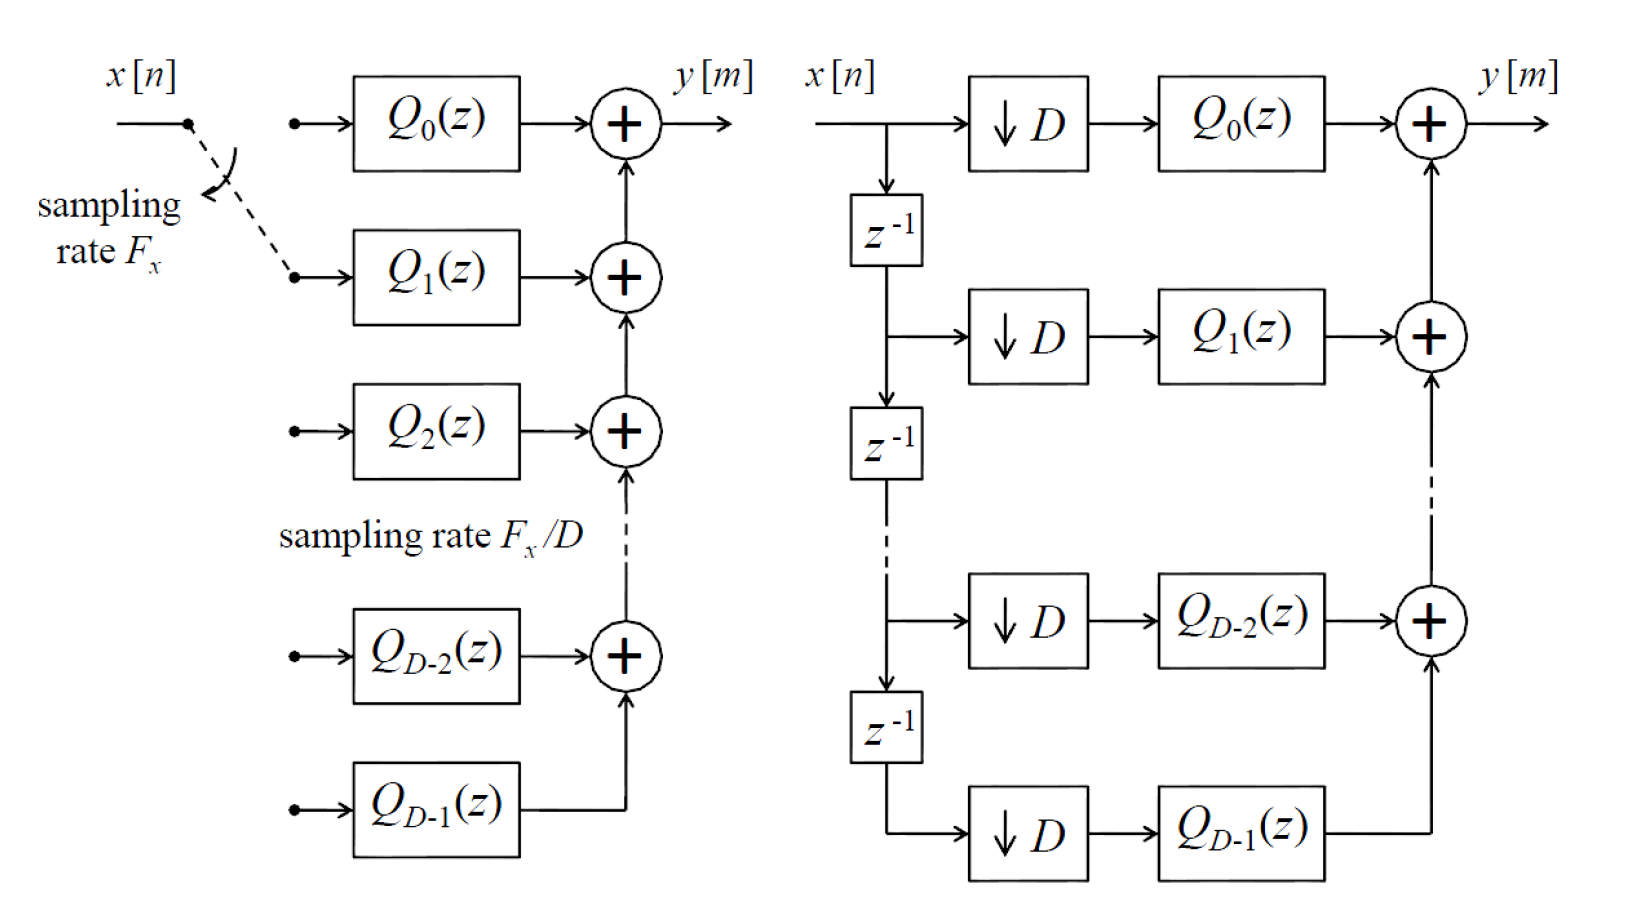
\includegraphics[width=\textwidth]{../fig/polyphase_down}
\end{minipage}
\newpage

%===============================================================================
\section{Implementation rationaler Abtastraten}
Wenn ein up- bzw. downsample Faktor gefordert ist, welcher nicht ganzzahlig ist,
kann dieser mit $\frac{I}{D}$ dargestellt werden.\\\\
Wenn zuerst der Downsampler kommt, gehen Informationen verloren. Andersrum
entsteht eine hohe Abtastfrequenz dazwischen. Es ist jedoch vorzuziehen,
zuerst das Upsampeln durchzuführen, danach das Downsamplen. So kann der Tiefpass 
der Interpolation mit dem Tiefpass der Decimation kombiniert werden.
\begin{center}
	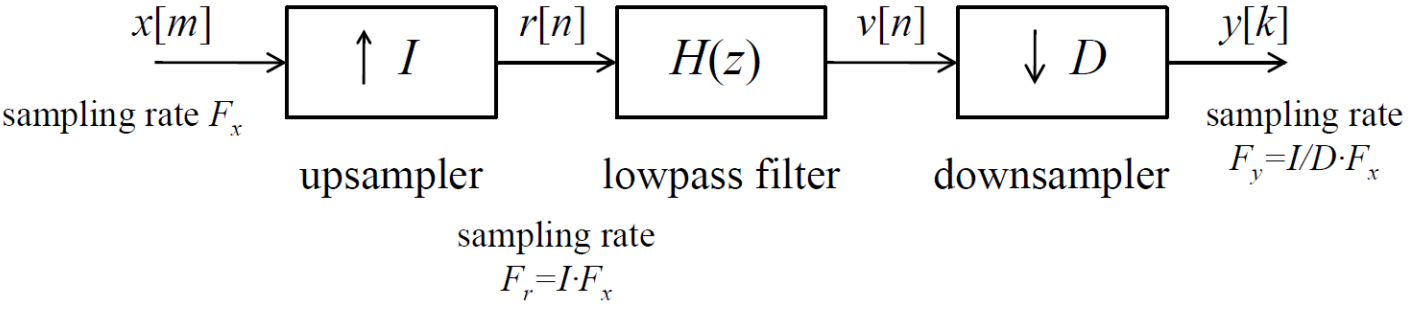
\includegraphics[width=.6\textwidth]{../fig/sampling}
\end{center}
Die Anzahl an Koeffizienten $p$ für einen FIR-TP-Filter mit Länge $N$ berechnet sich wie folgt:
\[ p = \frac{N}{I} \]
Es werden $p$ Multiplikationen sowie $p-1$ Additionen notwendig pro Output Sample des Filters.
%===============================================================================
\section{Quadratur Spiegel Filterbank}
Um den Datenverlust beim Downsampeln zu kompensieren, kann das Signal über zwei
Kanäle übertragen werden. Der eine Kanal filtert das Signal mit einem TP $H_0(z)$,
der Andere mit einem HP $H_1(z)$.
\begin{center}
	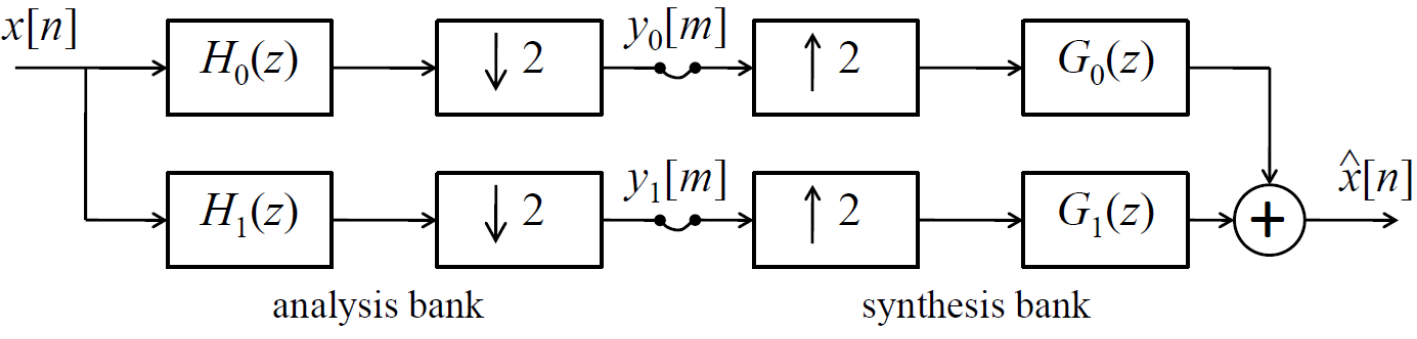
\includegraphics[width=.6\textwidth]{../fig/quadrature_mirror}
\end{center}
Die DTFT der zwei generierten Signalen $y_0[m]$ und $y_1[m]$ sind:
\[ Y_{0/1} = \frac{1}{2} \left( H_{0/1}\left( \frac{\Omega}{2} \right)
	X\left( \frac{\Omega}{2} \right) + H_{0/1}\left( \frac{\Omega}{2} - \pi
	\right) X\left( \frac{\Omega}{2} -\pi\right) \right)\]
Das Spektrum des synthetisierten Signals $\hat{x}[n]$ ist:
\[\begin{aligned} \hat{X}(\Omega) = &\frac12 \bigg( H_0(\Omega)G_0(\Omega)
	+ H_1(\Omega)G_1(\Omega) \bigg) \cdot X(\Omega) \\
	+ &\underbrace{\frac12 \bigg( H_0(\Omega-\pi)G_0(\Omega)
	+ H_1(\Omega-\pi)G_1(\Omega) \bigg) \cdot X(\Omega-\pi)}_
	{\textrm{alias term}} \end{aligned}\]
Um keinen Aliasterm zu haben müssen die Bedingungen $G_0(\Omega) = H_1(\Omega
-\pi)$ und $G_1(\Omega) = -H_0(\Omega-\pi)$ erfüllt sein.\\
Oft wird ebenfalls nur ein Filter $H(\Omega)$ gewählt. 
Meist wird dieses im $z$-Bereich bestimmt/vorgegeben und kann dann
mit $z=e^{j\cdot \Omega}$ umgewandelt werden.
Die entsprechenden Filter können dann wie folgt abgeleitet werden:
\[\begin{aligned}
	H_0(\Omega) &= H(\Omega)\\
	H_1(\Omega) &= H(\Omega-\pi)\\
	G_0(\Omega) &= H(\Omega)\\
	G_1(\Omega) &= -H(\Omega-\pi)
\end{aligned}\]
Anschliessend werden sie in den $z$-Bereich zurücktransformiert, z.B. 
$H_0(\Omega) \ \laplace \ H_0(z)$ oder $G_1(\Omega) \ \laplace \ G_1(z)$.\\
Dank dieser Transformation können die Impulsantworten einfach ermittelt werden.
\newpage \noindent
Weiter gilt für das synthetisierte Signalspektrum:
\[ \hat{X}(\Omega) = T(\Omega)X(\Omega) \qquad \text{, wobei: } 
				T(\Omega) = \frac{1}{2}\bigg(H^2(\Omega) -H^2(\Omega-\pi)\bigg) \]
Um perfekte Rekonstruktion zu haben, muss $T(\Omega)$ eine Allpass-
Charakteristik mit linearer Phasenverschiebung aufweisen (konstante Amplitudenverstärkung, konstante Zeitverzögerung). 
Dies kann am besten mit einem symmetrischen FIR-Filter (ungerade Ordnung) erreicht werden. Der einseitige Frequenzgang
sieht dann wie folgt aus:
\begin{center}
	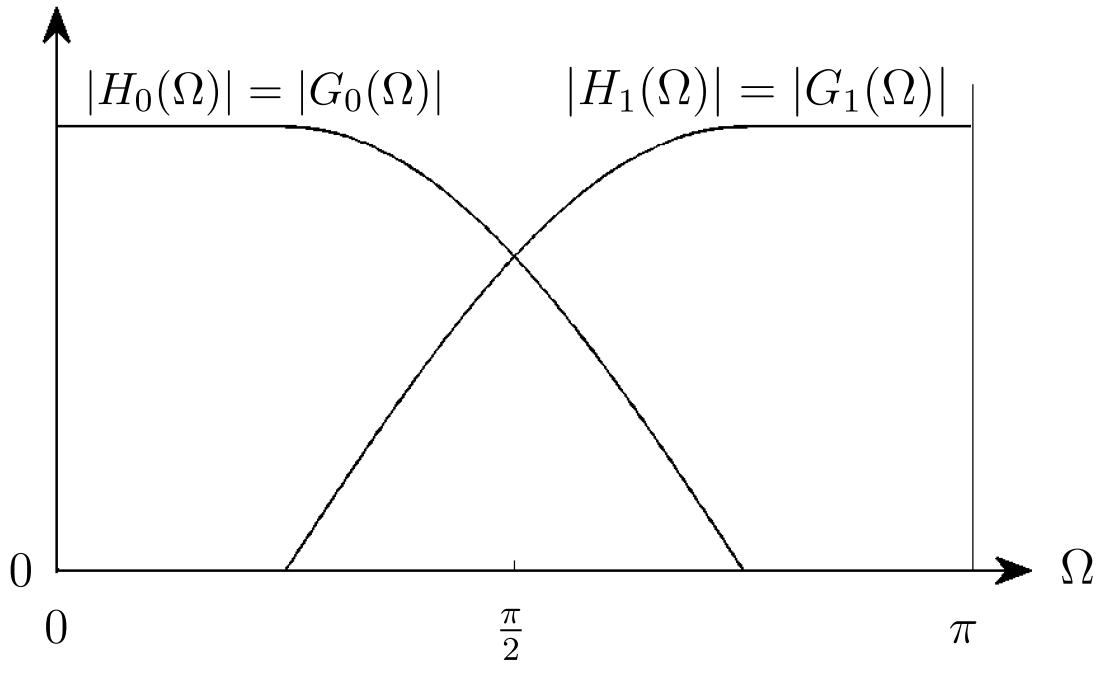
\includegraphics[width=.5\textwidth]{../fig/power_symetric}
\end{center}
Diese Filter werden z.B. in der Speicherung von Sprachsignalen verwendet. 
Dabei werden Signale in einzelne Frequenzbänder zerlegt. Tiefere Frequenzen 
kommen dabei vermehrt vor und können so besser (mehr Bits) quantisiert werden.
\begin{center}
	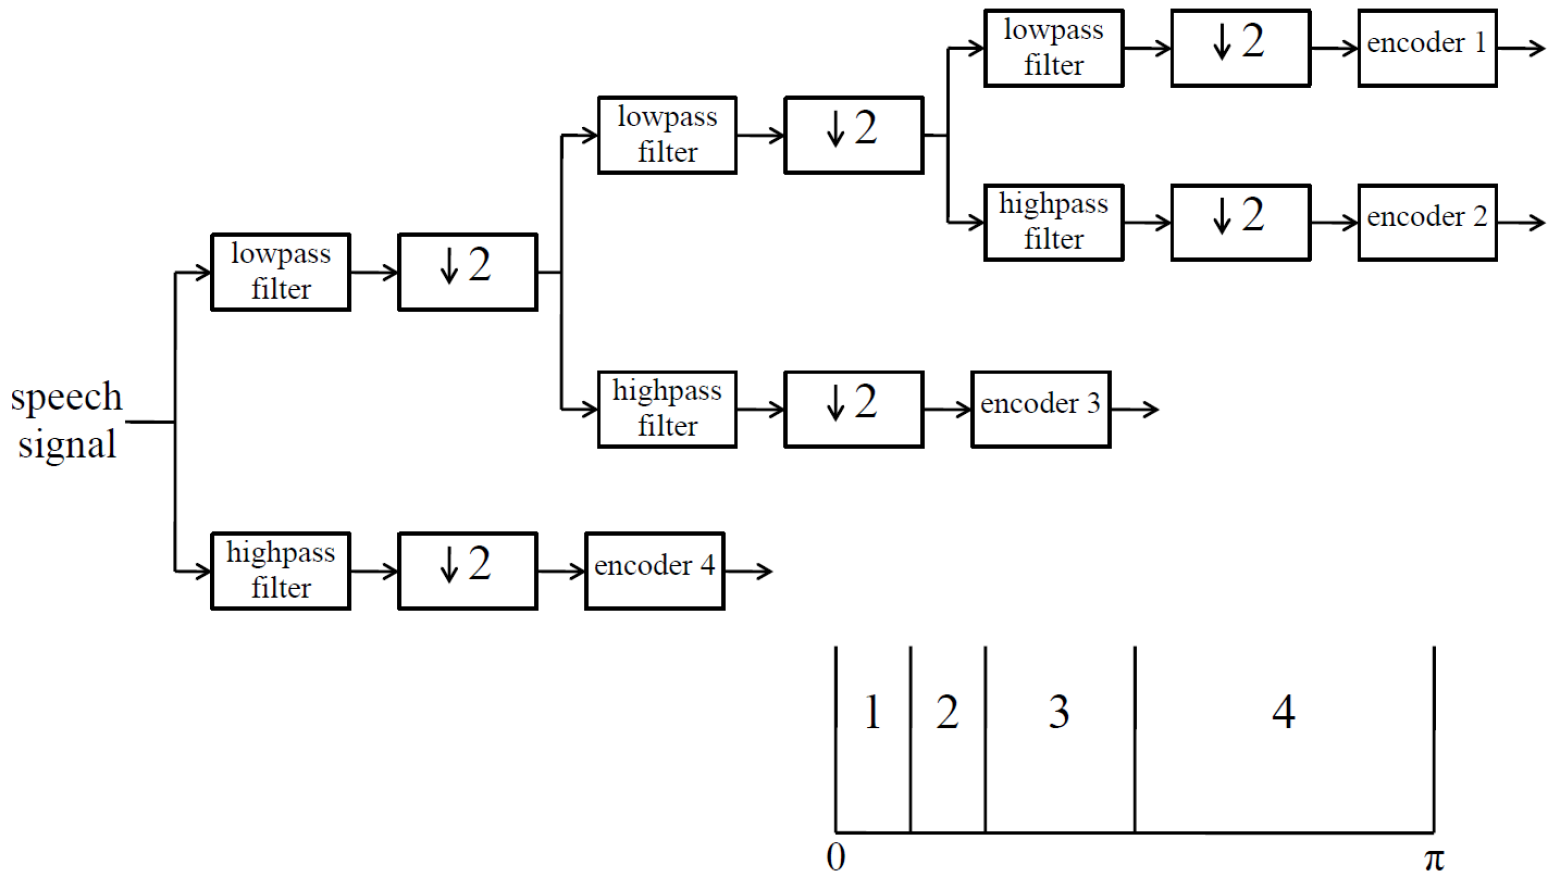
\includegraphics[width=.7\textwidth]{../fig/quadrature_mirror_ex}
\end{center}

%===============================================================================
\section{DFT Filterbank}
Bei dieser Filterbank handelt es sich un eine Generalisierung der Quadratur Spiegel
Filterbank. Die Anzahl Channels wird von $2$ auf $M$ erhöht. Es ergeben sich $M$ 
Filter in der Analyse \& Synthese. Die Subband-Signale können dadurch mit tieferer 
Sampling-Rate abgetastet werden. Es wird unterschieden zwischen:
\begin{itemize}[noitemsep,topsep=3pt]
	\item \textbf{Critical sampling:} Die Anzahl der Filter $H_0(z), H_1(z), \ldots, H_
{M-1}$ entspricht dem Downsampling $M$.
	\item \textbf{Oversampling:} Anzahl Kanäle ist grösser als der Downsampling Faktor.
	\item \textbf{Undersampling:} Anzahl Kanäle ist kleiner als der Downsampling Faktor. 
\end{itemize}
Mit Undersampling ist \emph{keine} perfekte Rekonstruktion des Eingangssignals $x[n]$ 
möglich.
\begin{center}
	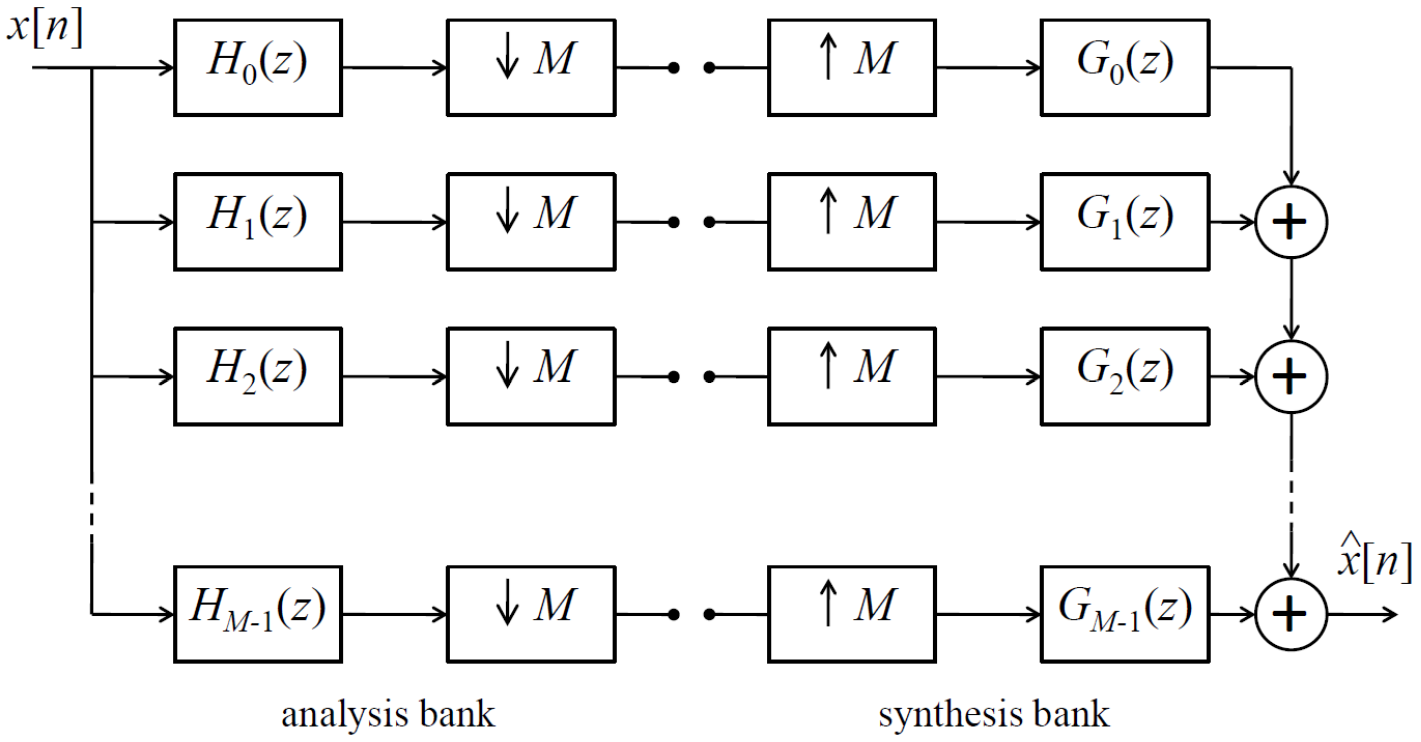
\includegraphics[width=.6\textwidth]{../fig/critical_sampled}
\end{center}
Um ein simpleres Design zu erreichen, wird der Prototype-Filter $H(z)$ (TP) jeweils 
frequenzmässig verschoben. Das selbe gilt für die Synthesis-Bank mit $G(z)$. 
\[ H_l(z) = H(z\cdot\e^{-\im 2\pi l/M}) \qquad l=0,1,\ldots,M-1 \]
\[ G_l(z) = G(z\cdot\e^{-\im 2\pi l/M}) \qquad l=0,1,\ldots,M-1 \]
\begin{center}
	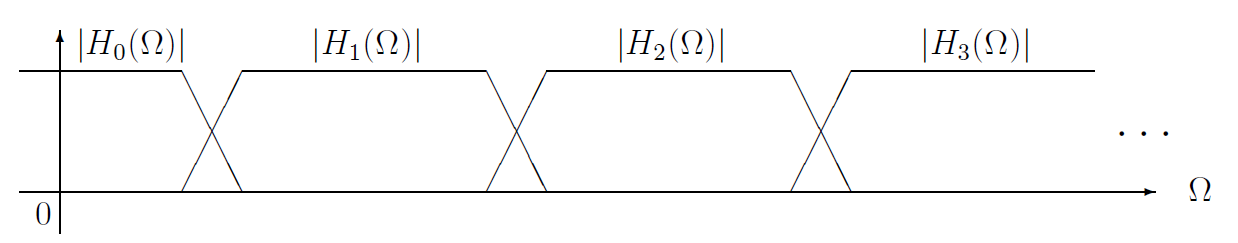
\includegraphics[width=.7\textwidth]{../fig/dft_bank_freq.png}
\end{center}
Frequenzgang:
\[ H_l(\Omega) = H(\Omega-2\pi l/M) \]
Die Namensgebung ist auf die folgende Implementierung zurückzuführen. Das Eingangssignal
wird im $l$-ten Kanal um $2\pi l/M$ geshiftet.
\begin{center}
	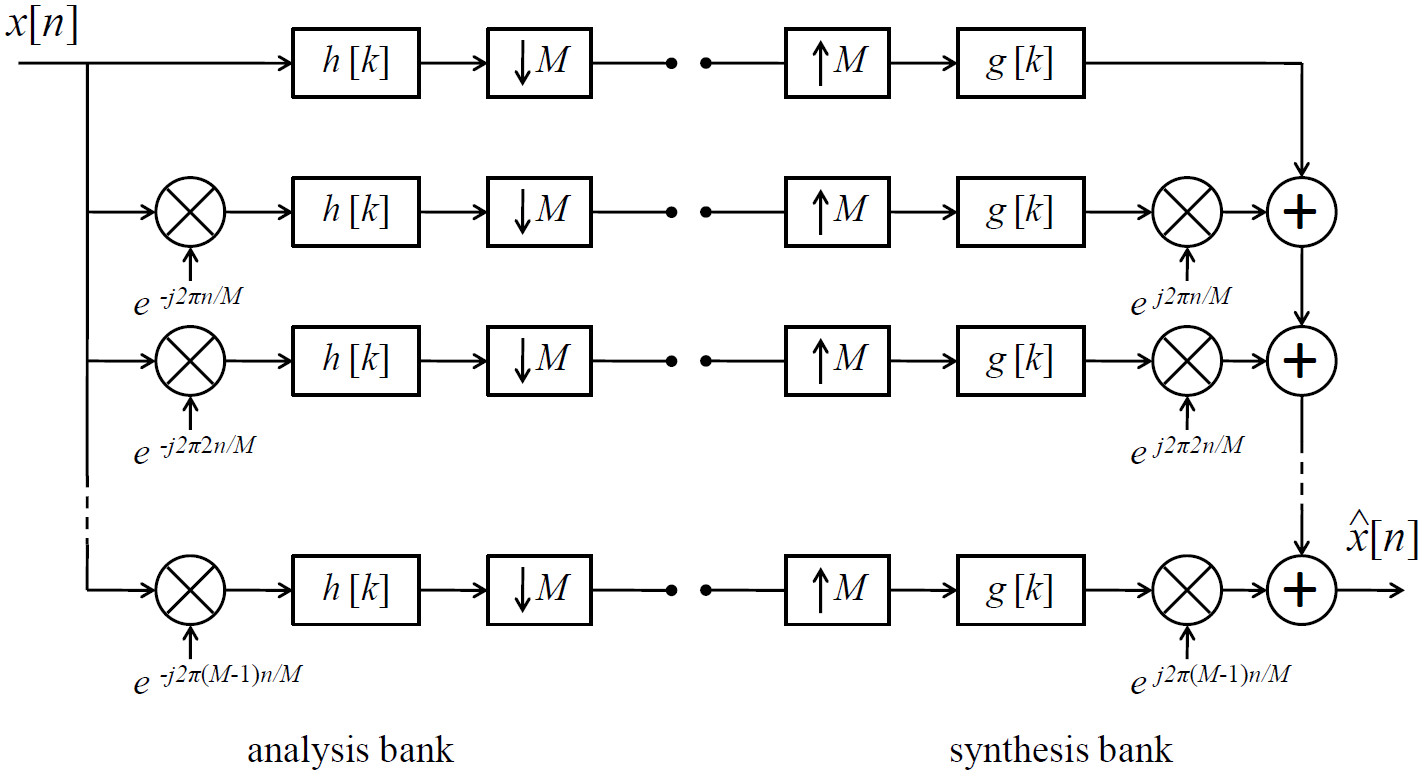
\includegraphics[width=.7\textwidth]{../fig/dft_filterbank_implementation.png}
\end{center}
Die Impulsantworten der Analysis \& Synthesis-Filter lauten:\\
\begin{minipage}{.5\textwidth}
	\[ h[k] = \left\lbrace\begin{matrix}
		1	& \textrm{if } k \in \{0,1,\ldots,M-1\}\\
		0	& \textrm{otherwise}
	\end{matrix}\right. \]
\end{minipage}
\begin{minipage}{.5\textwidth}
	\[ g[k] = \left\lbrace\begin{matrix}
		\frac{1}{M}	& \textrm{if } k \in \{0,1,\ldots,M-1\}\\
		0	& \textrm{otherwise}
	\end{matrix}\right. \]
\end{minipage}
\newpage \noindent

Mit Polyphase kann dies in eine DFT mit Polyphase Filter aufgeteilt werden:
\[ H_l(z) = \sum_{i=0}^{M-1}\e^{\im 2\pi li/M} \cdot (z^{-i} \cdot P_i(z^M) )
	\qquad l=0,1,\ldots,M-1 \]
\begin{minipage}{.6\textwidth}
	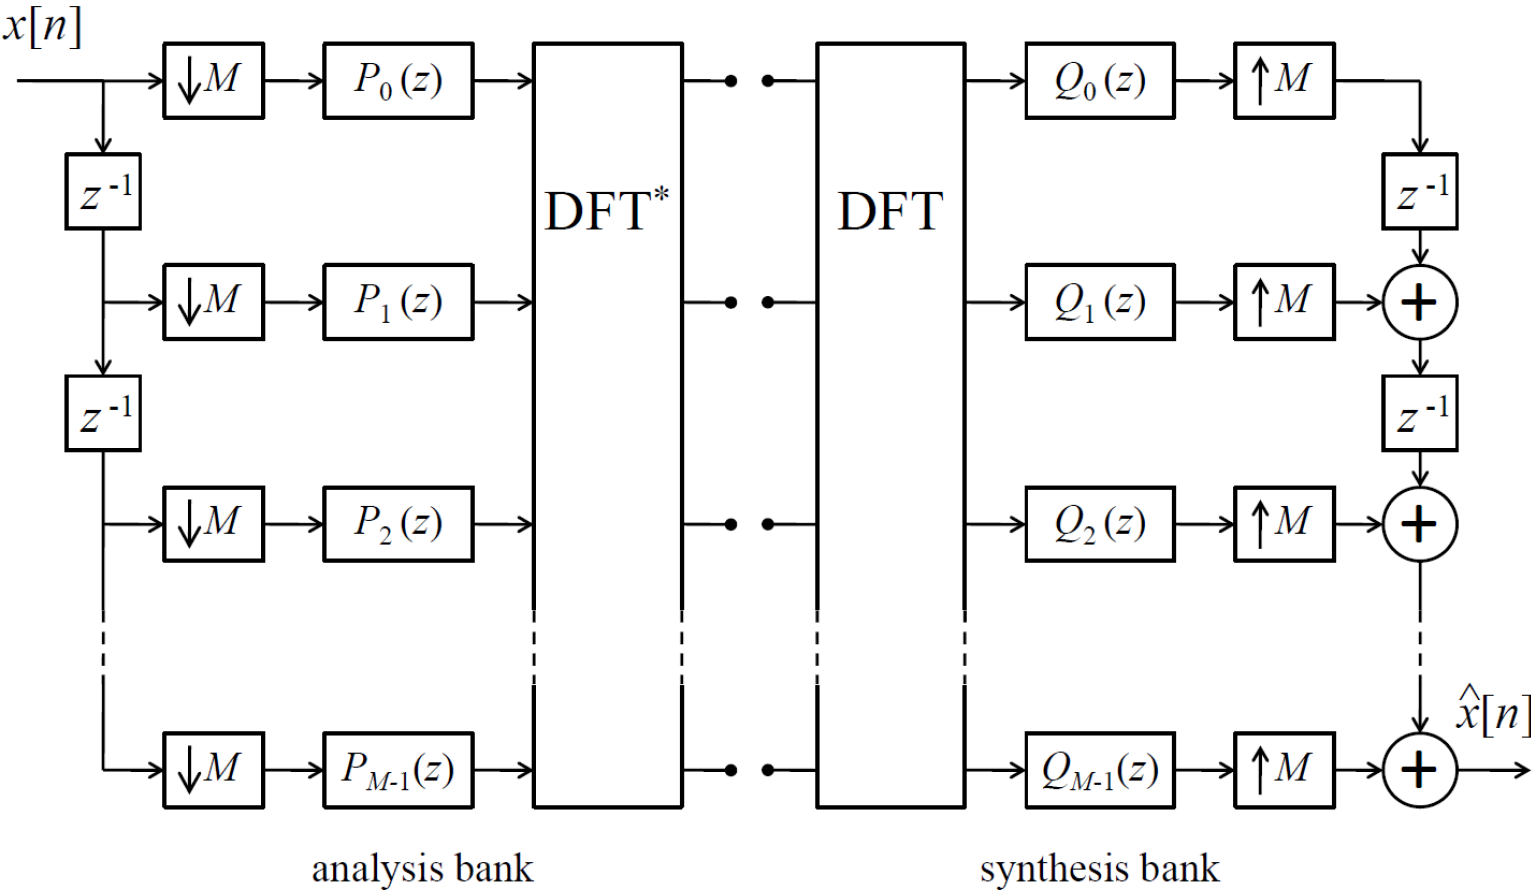
\includegraphics[width=\textwidth]{../fig/dft_filterbank}
\end{minipage}
\begin{minipage}{.4\textwidth}
	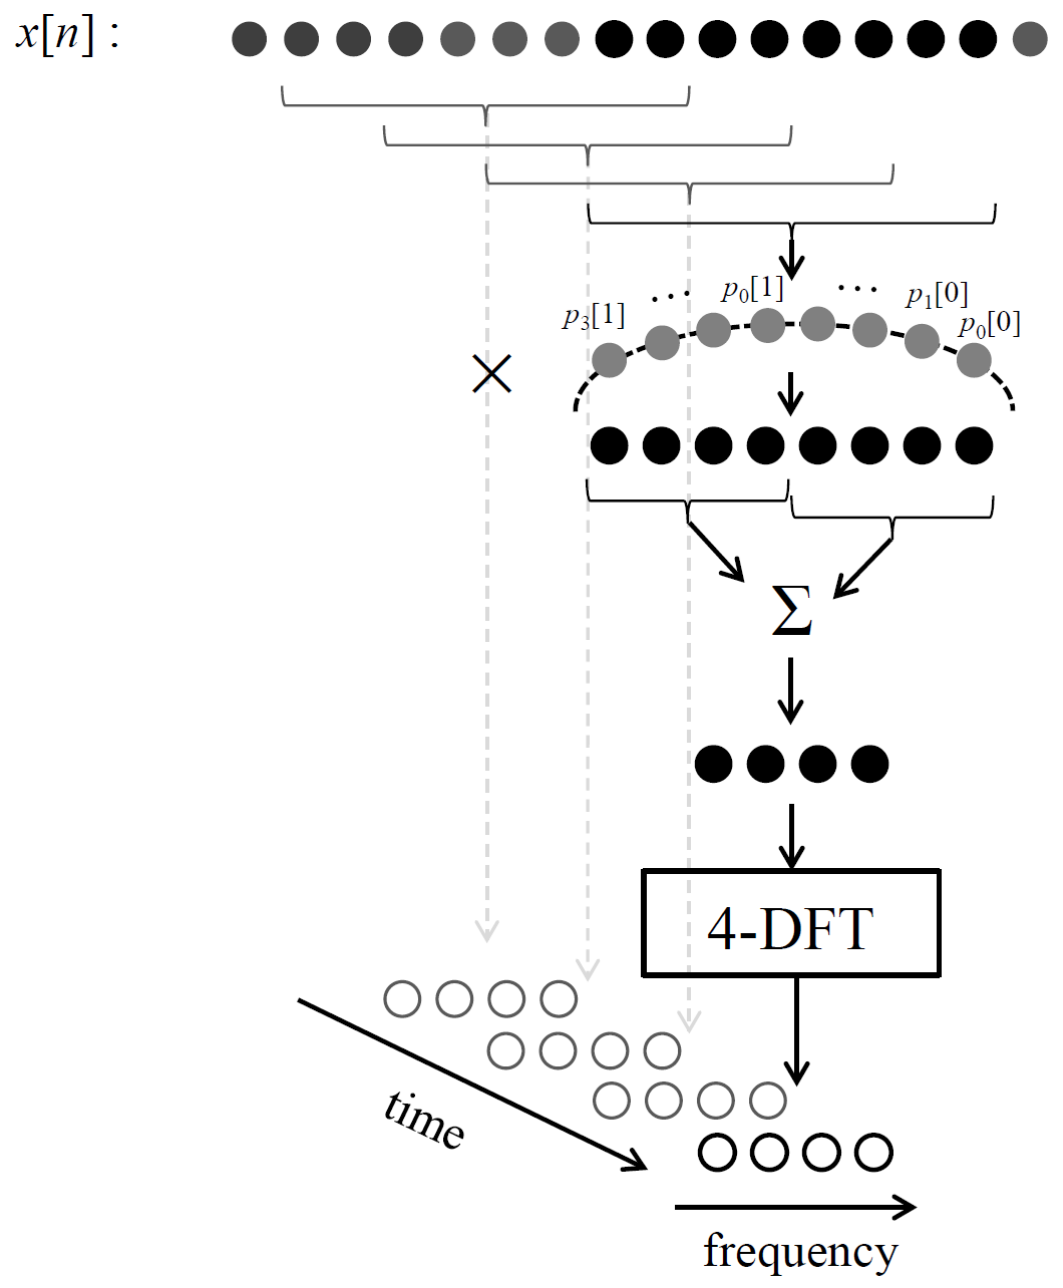
\includegraphics[width=\textwidth]{../fig/dft_filter_ill}
\end{minipage}
Filterbank Ausgangssignal im $z$-Bereich:
\[ \hat{X}(z) = \sum_{i=0}^{M-1}z^{-i} \cdot Q_i(z^M) \cdot \sum_{i=0}^{M-1}Y_l(z^M) \cdot e^{j2\pi li/M} \]
~\\
Vorteile der DFT-Filterbank mit Polyphasen-Struktur:
\begin{itemize}[noitemsep,topsep=3pt]
	\item Es handelt sich um FIR-Filter bei den Polyphase-Komponenten. Dabei handelt es sich um downgesampelte Varianten
	von $h[k]$ und $g[k]$. Diese Filter haben typischerweise einen kleinen Komplexitätsgrad. 
	\item Für die DFT-Berechnungen sind effiziente FFT-Algorithmen verfügbar.
\end{itemize}
% coding:utf-8

%----------------------------------------
%FOSADSVB, a LaTeX-Code for a summary of digital signal processing
%Copyright (C) 2015, Mario Felder & Michi Fallegger

%This program is free software; you can redistribute it and/or
%modify it under the terms of the GNU General Public License
%as published by the Free Software Foundation; either version 2
%of the License, or (at your option) any later version.

%This program is distributed in the hope that it will be useful,
%but WITHOUT ANY WARRANTY; without even the implied warranty of
%MERCHANTABILITY or FITNESS FOR A PARTICULAR PURPOSE.  See the
%GNU General Public License for more details.
%----------------------------------------

\chapter{Zufallssignale}
\section{Autokorrelation und Spektrum}
Mittelwert eines Zufallssignals $x[n]$ ist
\[ m_x = E\{x[n]\} \]
Autokorrelation
\[ \gamma_{xx}[m] = E\{x^*[n] \cdot x[n+m]\} \]
Wobei $\gamma_{xx}[0]$ die Leistung $P_x$ repräsentiert.\\\\
Für echte Zufallssignale gilt
\[ \gamma_{xx}[m] = \gamma_{xx}^*[-m] \]
Signale, welche den Mittelwert nicht bei Null haben, werden mit der Autokovarianz
charakterisiert
\[ c_{xx} = E\{ (x[n]-m_x)^*\cdot(x[n+m]-m_x) \} \]
\[ y_{xx} = c_{xx}[m] + _x^2 \]
Die Autokovarianz bei $m=0$ repräsentiert die Varianz
\[ E\{|x[n]-m_x|^2\} \]
Spektrum durch die DTFT im Intervall $[n_1,n_2]$
\[ X_{[n_1,n_2]}(\Omega) = \sum_{n=n_1}^{n_2}x[n]\cdot\e^{\im\Omega n} \]
Leistungsdichte Spektrum (power density spectrum)
\[ \Gamma_{xx}(\Omega) = \sum_{m=-\infty}^{\infty}\gamma_{xx}[m] \cdot
	\e^{-\im\Omega m} \]
~\\\\
Weisses Rauschen hat die Autokorrelation
\[ \gamma_{ww}[m] = \left\lbrace\begin{matrix}
	\sigma_w^2	& \textrm{if } m = 0\\
	0			& \textrm{if } m \neq 0
\end{matrix}\right. \]
Das Leistungsdichte Spektrum beim seissen Rauschen ist über $\Omega$ konstant.

%===============================================================================
\section{Spectral Shaping in LTI Systems}
Mittelwert des Ausgangssignals $y[n]$:
\[ m_y = H(0) \cdot m_x \]
mit
\[ H(\Omega) = \sum_{k=-\infty}^{\infty}h[k]\cdot\e^{\im\Omega k} \]
Autokorrelation von $y[n]$
\[ \gamma_{yy}[m] = h^*[-i]*\gamma_{xx}[m]*h[k] \]
Frequenzbereich
\[ \Gamma_{yy}(\Omega) = H^*(\Omega)\cdot\Gamma_{xx}(\Omega)\cdot H(\Omega) 
	= |H(\Omega)|^2 \cdot \Gamma_{xx}(\Omega) \]
	
%===============================================================================
\section{Lineare Modelle für Stochastische Prozesse}
Weisses Rauschen
\[ \Gamma_{ww}(z) = \sigma_w^2 \]
Ausgang des LTI
\[ \Gamma_{yy}(z) = \sigma_w^2 \cdot H(z) \cdot H(z^-1) \]
Weisses Rauschen kann erzeugt werden, indem ein bekanntes Zufallsignal mit
\[ \frac{1}{H(z)} \]
multipliziert wird. Ergibt für die Differenzengleichung
\[ w[n] = \frac{1}{b_0}\left( y[n] + \sum_{k=1}^{N}a_ky[n-k] - 
	\sum_{k=1}^{M}b_kw[n-k] \right) \]
	
%===============================================================================
\subsection{Moving average model}
$H(z)$ ist ein FIR Filter mit Ordnung $M$ welcher ein weisses Rauschen $w[n]$
in ein Zufallsignal transformiert:
\[ y[n] = \sum_{k=0}^{M}b_kw[n-k] \]
Im spezial Fall $b_0=b_1=\ldots=b_M=(M+1)^{-1}$ repräsentiert jedes Sample des
Filterausgans der Durchschnitt des Eingangsignals in einem verschiebbaren
Fenster der Länge $M+1$.\\
\\
Berechnung der Koeffizienten bei gegebener Autokorrelation $\gamma_{yy}$:
\[ \gamma_{yy}[m] = \left\lbrace \begin{matrix}
	\sigma_w^2\sum_{k=m}^{M}b_k\cdot b_{k-m}^* & \textrm{if } 0\leq m \leq M\\
	0	& \textrm{if } m > M\\
	\gamma_{yy}^*[-m]	& \textrm{if } m < 0
\end{matrix}\right. \]

%===============================================================================
\subsection{Autoregressive model}
Zufallssequenz ist durch einen All-pole Filter generiert:
\[ y[n] = w[n] - \sum_{k=1}^{N}a_ky[n-k] \]
Hat keine Pole und ist immer stabil.\\
Berechnung der Koeffizienten bei gegebener Autokorrelation $\gamma_{yy}$:
\[ \gamma_{yy}[m] = \left\lbrace \begin{matrix}
	-\sum_{k=1}^{N}a_k\cdot\gamma_{yy}[m-k] & \textrm{if } m>0\\
	\sigma_0^2-\sum_{k=1}^{N}a_k\cdot\gamma_{yy}[m-k] & \textrm{if } m =0\\
	\gamma_{yy}^*[-m]	& \textrm{if } m < 0
\end{matrix}\right. \]
Das Lösungsystem in Matrizenform:
\[ \begin{bmatrix}
	\gamma_{yy}[0] & \gamma_{yy}[-1] & \ldots & \gamma_{yy}[-N]\\
	\gamma_{yy}[1] & \gamma_{yy}[0] & \ldots & \gamma_{yy}[-N+1]\\
	\vdots & \vdots & & \vdots\\
	\gamma_{yy}[N] & \gamma_{yy}[N-1] & \ldots & \gamma_{yy}[0]
\end{bmatrix} \cdot \begin{bmatrix}
	1 \\ a_1 \\ \vdots \\ a_N \end{bmatrix} = \begin{bmatrix}
	\sigma_w^2 \\ 0 \\ \vdots \\ 0 \end{bmatrix} \]  
	
%===============================================================================
\subsection{ARMA model}
Ist die Zusammensetzung des MA und AR Models. Dabei sind die Ordnungen der
Polynomen $B(z)$ und $A(z)$ 1 oder höher. Somit hat der Pol-Nullstellenplan
Nullen und Pole. Dieser ist allerdings geeigneter als die Spezialfälle MA und
AR, da weniger Koeffizienten für ein gutes Model benötigt werden.

\end{document}

